\chapter{Simulation and Analytical Modeling of HELIOS Reflectors} \label{Simulation and Analytical Modeling of HELIOS Reflectors}
This section develops an analytical model for the reflection behavior of HELIOS reflectors that are co-designed/validated via numerous EM simulations. First, we introduce the methodology of this in \Cref{sec:Simulation Methodology}. After laying the groundwork, \Cref{Simulative Analyses of HELIOS Reflector Modules} studies key reflection characteristics of HELIOS reflectors using an EM simulator.  Thereafter, \Cref{Analytical Modeling of HELIOS Modules} develops an analytical model for the reflection of individual HELIOS modules by building upon an existing radar cross-section formulae for flat plates and extending it according to the prior simulation results. Lastly, \Cref{Simulation and Modeling of HELIOS Reflectors} extends the analytical model to HELIOS reflectors to make up an array of individually parameterized modules. The thesis would focus on considering the self-shadowing effects that may occur between neighboring modules.
\section{Methodology}\label{sec:Simulation Methodology}
It is crucial to recognize that HELIOS is made up of a collection of HELIOS modules that all follow the same geometry template \cite{Helios}. However, the study draws attention to the unique feature that these modules may have different $\alpha$ and $\beta$ slopes. The corresponding paragraphs of \Cref{Passive reflectors} provide a more thorough explanation of this deviation from uniformity, highlighting the importance of these subtle adjustments to the overall structure and functionality of the HELIOS array. Using the author's definition in \cite{Helios}, we have constructed and integrated the geometry in the Ansys HFSS software which is a commercial EM simulation tool. We use the simulator as the fundamental physical prediction of the exhibited HELIOS reflection pattern which is strongly dependent on the geometry but also the angles of arrival of the incident EM wave.

The analytical modeling of the reflection behavior of arbitrarily configured HELIOS reflectors in \Cref{Analytical Modeling of HELIOS Modules}, and \Cref{Simulation and Modeling of HELIOS Reflectors} relies heavily on these simulative insights, particularly our initial detailed simulation study in \Cref{Simulative Analyses of HELIOS Reflector Modules}. Owing to this, we now outline the simulation workflow being used to attain the results presented in the forthcoming sections. We note that other commercial EM simulation tools offer the same functionality and should therefore operate similarly.

\Cref{fig:SimulationFlow} sketches the parametrization of the EM simulations of the HELIOS reflectors, thus providing a methodical and data-driven approach to investigate how key performance metrics, extractable from the simulation results for the specified far-field observation range, depending on the reflector configuration. In the above figure, an external IronPython script is used to automate the simulations in this case, which provides the simulation configuration in terms of the parametrization of the HELIOS reflector configuration under test as well as the scenario in terms of the incident wave, reflection observation angle range, and operating frequency. Here, the frequency is typically \SI{28}{\giga\hertz}, which lies in the 5G n\num{257} mmWave frequency band. The saved results are then analyzed using the MathWorks MATLAB tool to draw sensible conclusions. This knowledge shall then be used during the development of the analytical model in \Cref{Analytical Modeling of HELIOS Modules}, and \Cref{Simulation and Modeling of HELIOS Reflectors}.

\begin{figure}[tb]
	\centering
	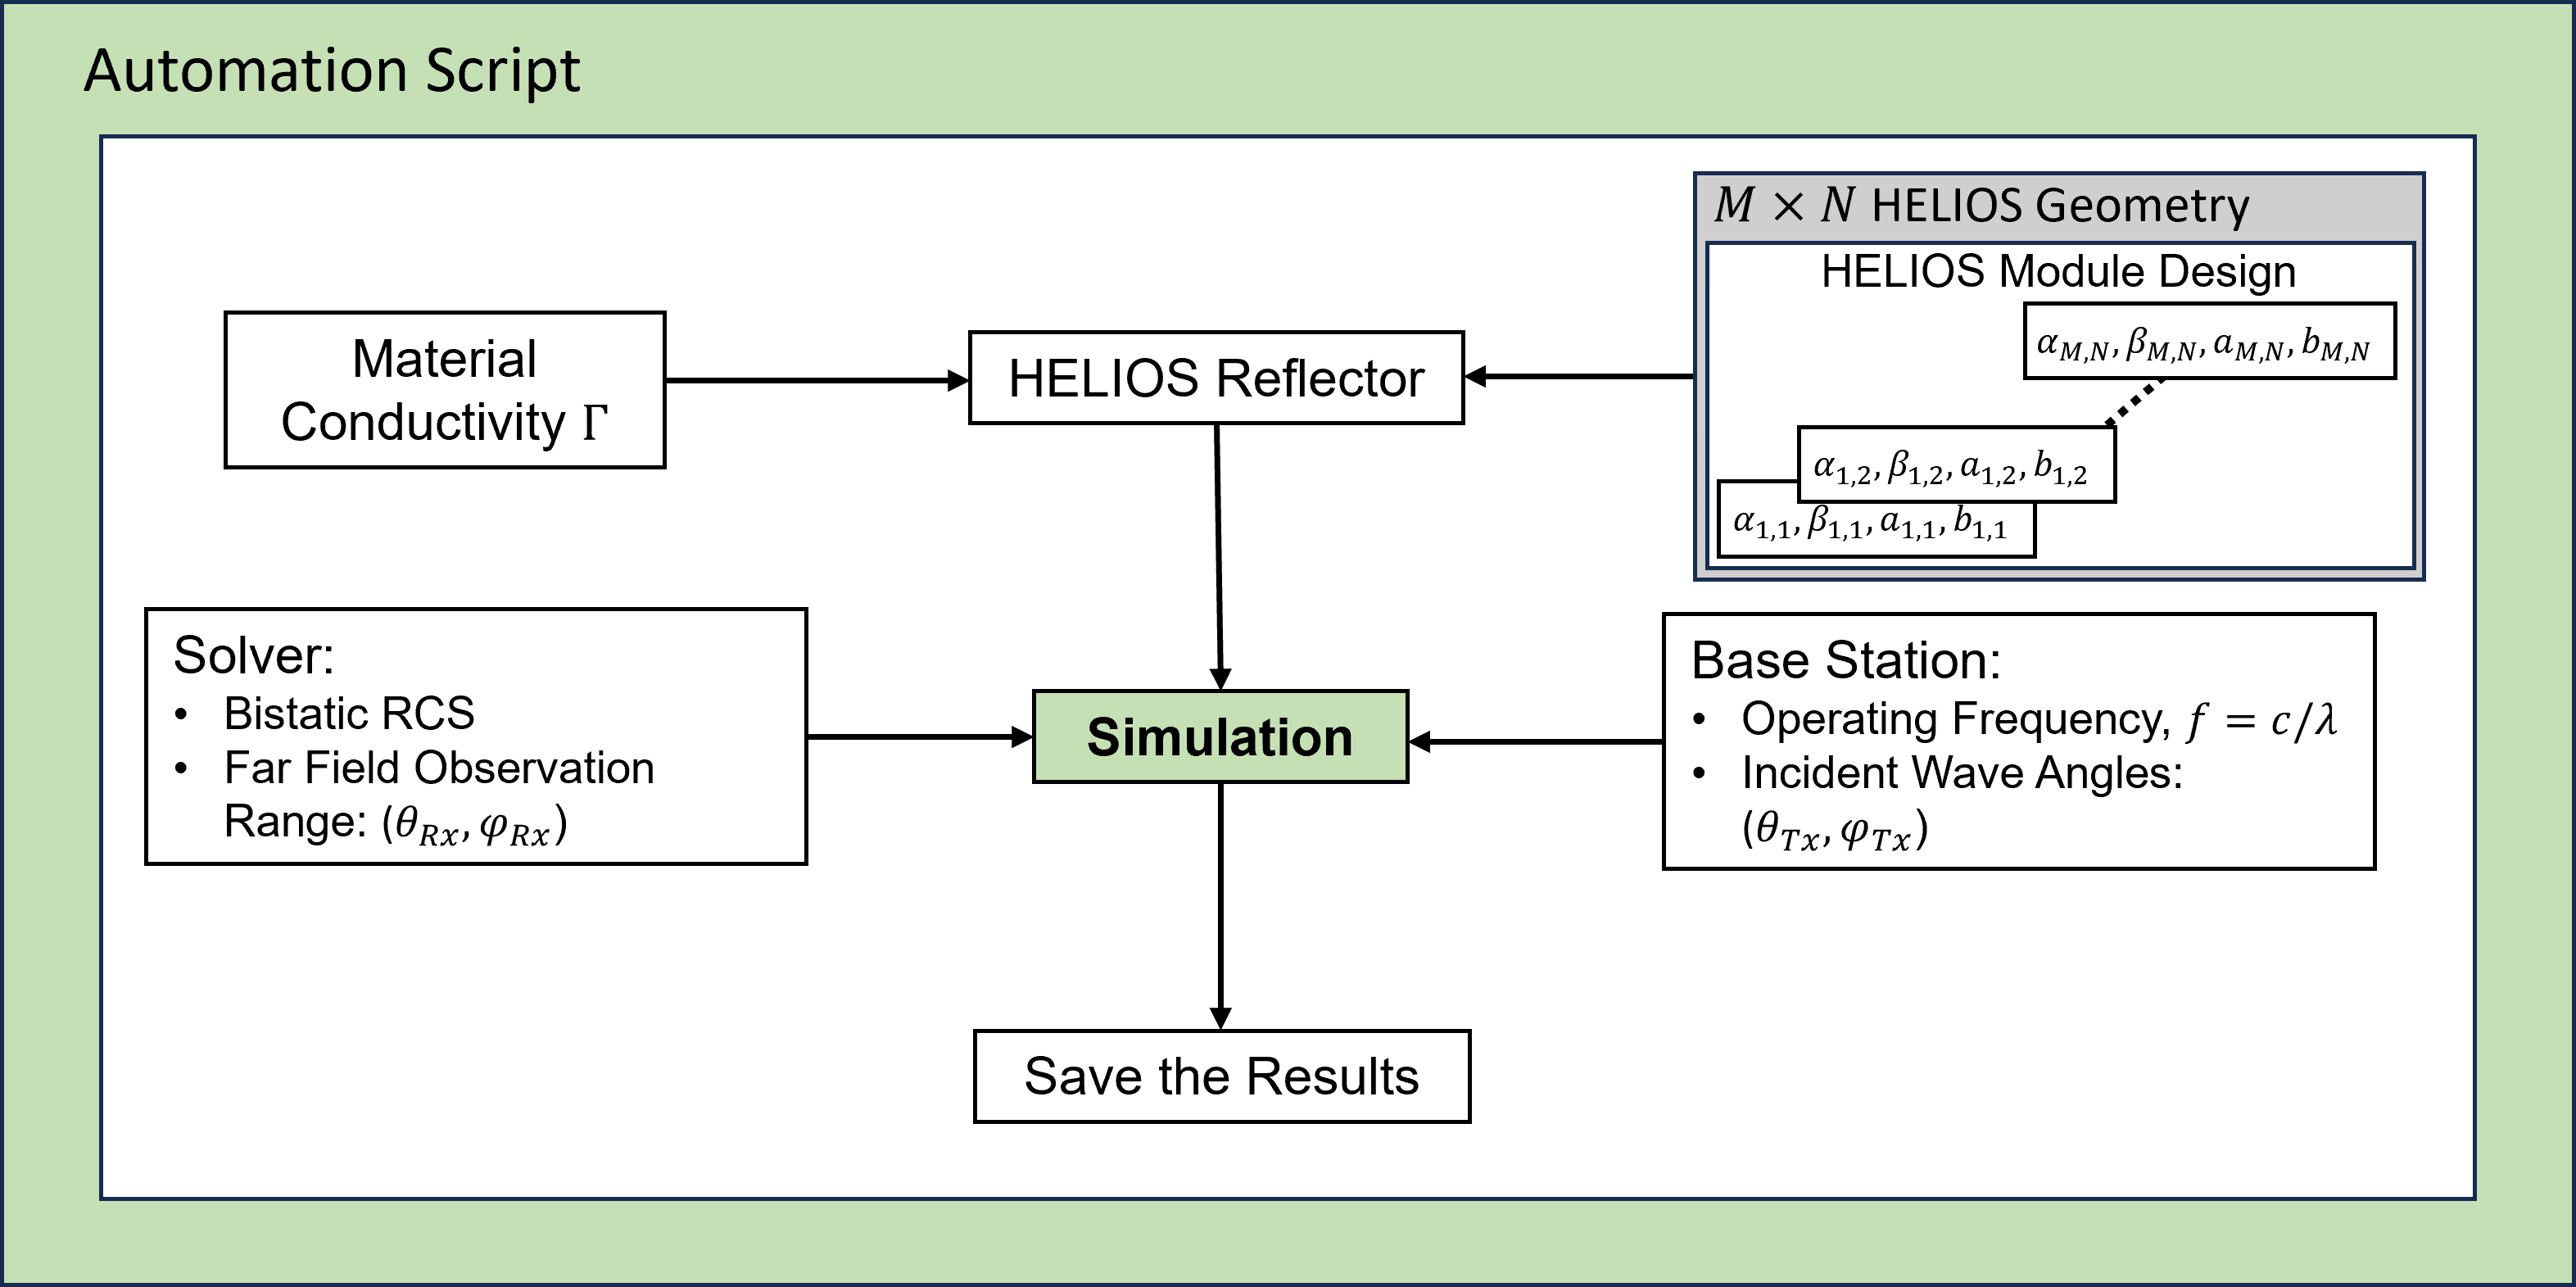
\includegraphics[width=1.0\linewidth]{images/Section 3 Images/Ansys_workflow}
	\caption{Illustration of the EM simulation workflow of the HELIOS reflectors. Simulation parameters in terms of base station configuration, far-field settings, and HELIOS reflector may be changed as desired for each simulation using an automation script.}
	\label{fig:SimulationFlow}
\end{figure}
Horizontal and vertical angles of incidence as well as of departure will all adhere to $\varphi_{Tx}, \theta_{Tx} \in [-90, 90]^\circ$ using the coordinate system defined in \Cref{coordinate systems}. These angles of incidence will be varied in this study to consider different deployment scenarios. The far-field observation range typically constitutes the half-sphere spanned by the above-defined range. Due to the simulation complexity, the resolution of simulation for this set of angles differs depending on, e.g., the HELIOS reflector size. For each of these points along the half-sphere, the EM simulator calculates the bistatic RCS (see \Cref{Analytical Modeling of HELIOS Modules}).

As discussed before, each HELIOS reflector element $\left(m,n\right)$ consists of four crucial parameters, i.e., dimensions $a_{m,n}$, and $b_{m,n}$ being the footprint sizes along $y$ and $z$-axes, respectively, and slopes $\alpha_{m,n}$, and $\beta_{m,n}$ constituting the horizontal and vertical slopes, respectively. The whole HELIOS reflector consists of $M \times N$ elements with $m\in1,\dots,M$ and $n \in 1, \dots, N$, cf. \Cref{Metasurfaces}. In this work, we assume that all individual elements have the same footprints, i.e., $a=a_{m,n}\in m,n$ and $b=b_{m,n} \in m, n$. Therefore, there are $2 \cdot N \cdot M + 2$ parameters constituting a HELIOS geometry. In the scope of \Cref{Simulative Analyses of HELIOS Reflector Modules}, the impact of selecting different common materials will be tested. In addition, artificial materials with arbitrary conductivity will be studied. Thereafter, copper will be used as the HELIOS baseline material as in \cite{Helios}.
The term "Gain" refers to the RCS, as elucidated in \Cref{Analytical Modeling of HELIOS Modules}, throughout this work. This application of the term gain is consistent with the definition given in \Cref{coordinate systems}, which presents a direct comparison of all three IRS models. A cohesive and seamless interpretation of the RCS behavior across different model comparisons is ensured by the study's maintenance of terminology compatibility.
\section{Simulative Analyses of HELIOS Reflector Modules} \label{Simulative Analyses of HELIOS Reflector Modules}
In this section, we thoroughly assess the reflection characteristics of a single-element HELIOS reflector to shed light on how it behaves for various parameter combinations. This section is divided into three sections, each of which focuses on a different component of the evaluation. The study looks into the effects of changing slope angles in \Cref{Variation of Slope Angle} to comprehend how these changes affect the system as a whole. In \Cref{Variation of Element Size}, the impacts of different reflector sizes are examined to determine how size variations affect the system's performance. In conclusion, \Cref{Impact of Material Conductivity} delves into the effects of altering the materials that make up the reflecting surface, thereby offering a comprehensive understanding of how distinct materials influence the overall performance and effectiveness of the reflective system.
%\begin{itemize}
%	\item \textbf{Variation concerning Slope Angle \textbf{$\alpha$}}
%	\item \textbf{Reflector Length Variation}
%	\item \textbf{Material Variations}
%\end{itemize}
%\begin{figure}
%	\centering
%	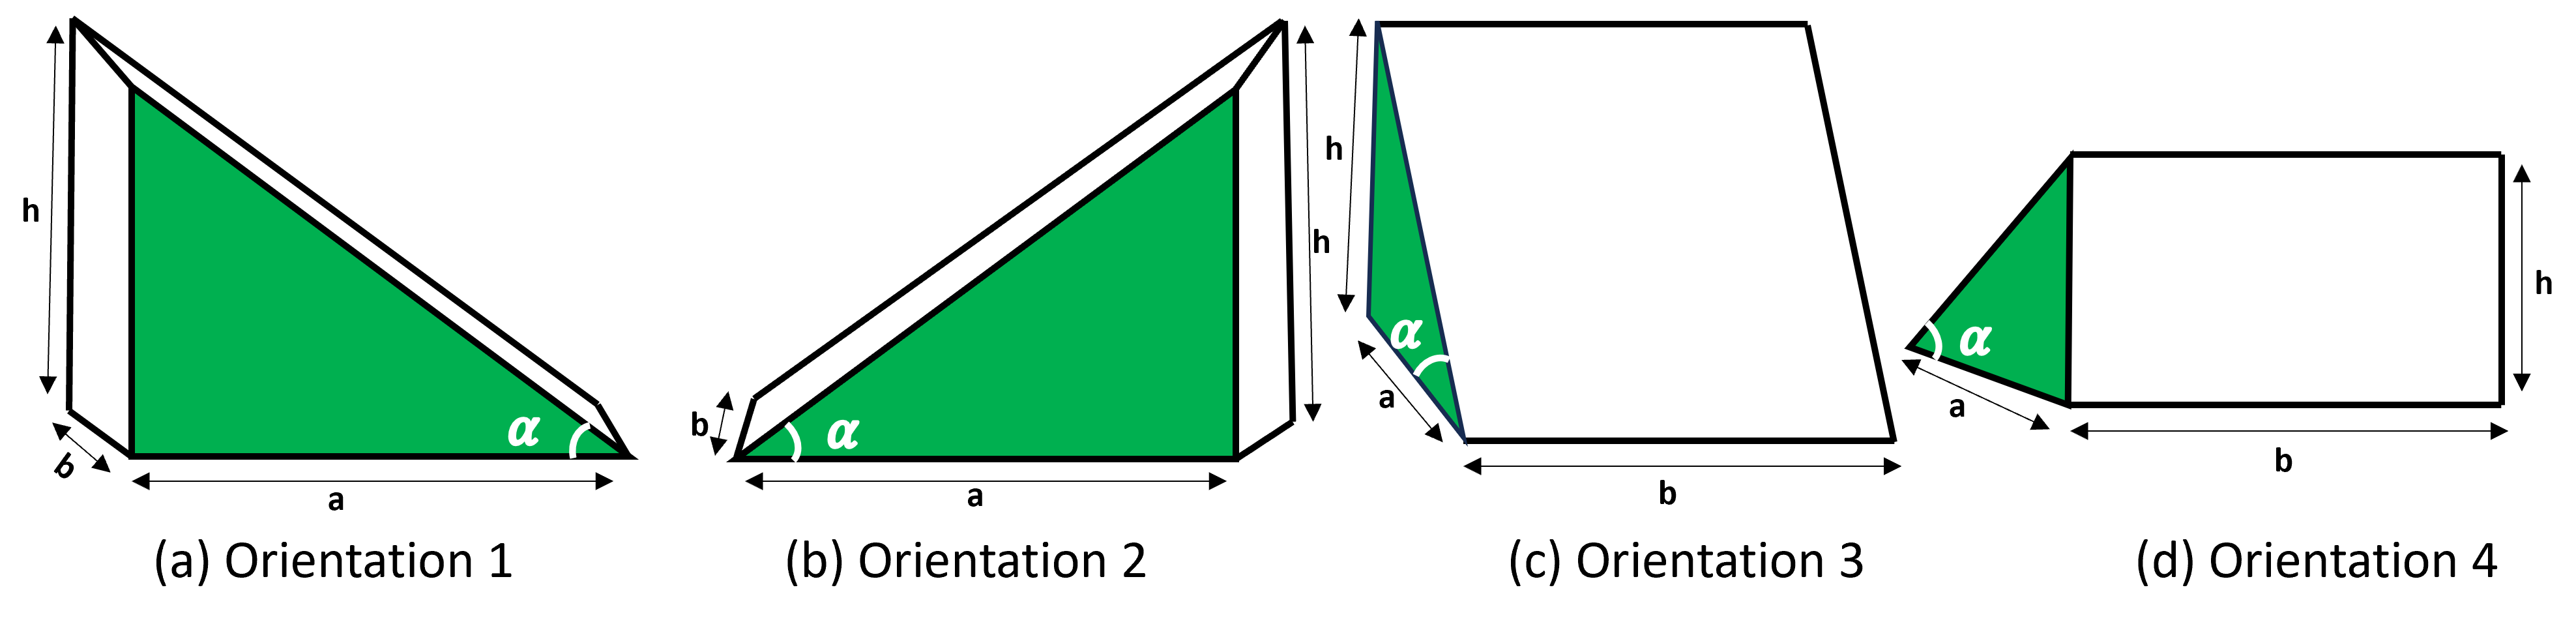
\includegraphics[width=1.0\linewidth]{images/Section 3 Images/orientations4}
%	\caption{Depicting the four variations of real-time implementations in orientations of a HELIOS module.}
%	\label{fig:orientations4}
%\end{figure}
\subsection{Variation of Slope Angle} \label{Variation of Slope Angle}
Using the fundamental HELIOS idea as a starting point, a significant departure from the established law of reflection i.e., $\varphi_{Rx} \neq -\varphi_{Tx}$ and $\theta_{Rx} \neq -\theta_{Tx}$ appears. \Cref{fig:HELIOS-model} shows the design of the HELIOS reflectors with the size of the reflectors $a$ and $b$ as well as the slope angles $\alpha$ and $\beta$, which are intricately related to the dimensions of the reflecting surface. The model here assumes that have incident wave is orthogonal to the reflector module base ($\theta_{Tx}=\varphi_{Tx}=0^\circ$). As presented by the authors in \cite{Helios}, this results in a noticeable change in the reflected angle by two times the slope angle, see \Cref{HELIOS 2times beta} and \Cref{HELIOS 2times alpha} below.
\begin{figure}[tb]
	\centering
	\includegraphics[width=0.7\linewidth]{images/Section 3 Images/HELIOS model}
	\caption{HELIOS module with the implementation of $\alpha$ and $\beta$ slope angles with incident wave orthogonal to the reflector base i.e., $\theta_{Tx}=\varphi_{Tx}=0^\circ$ and reflected wave validating HELIOS concept \cite{Helios} with two times shift in the slope angles.}
	\label{fig:HELIOS-model}
\end{figure}
\begin{equation} \label{HELIOS 2times beta}
	\theta_{Rx}=-\theta_{Tx}+2 \cdot \beta \\
\end{equation}
\begin{equation} \label{HELIOS 2times alpha}
	\varphi_{Rx}=-\varphi_{Tx}+2 \cdot \alpha \\
\end{equation}
In our first simulative study, we focus on the variation of the horizontal slope angle $\alpha$ within the range of $[\num{0}:\num{80}]^\circ$, in our effort to comprehend the complex dynamics of our HELIOS reflector modules. This investigation is essential in figuring out how slope angles affect the behavior of the model. Let us consider a simplified scenario where vertical slope angle $\beta=\num{0}^\circ$ is held constant to validate these intriguing results and the variation in $\varphi_{Rx}$ as a function of $\alpha$ to best illustrate the essence of this experiment (see \Cref{fig:saturation}). Notably, within the range of $\alpha$ from $\num{0}^\circ$ to $\num{45}^\circ$, \Cref{HELIOS 2times beta} and \Cref{HELIOS 2times alpha} accurately capture the behavior of the model. Beyond the $\num{45}^\circ$ threshold of $\alpha$, something different happens because the term $2 \cdot \alpha$ exceeds $\num{90}^\circ$.

This behavior as shown in \Cref{fig:saturation}, causes the beams to go beyond the limits of the considered far-field, resulting in a seeming saturation effect. The reason for this behavior is the energy being reflected behind the reflector which can be seen on the right side of the figure \Cref{fig:saturation}. As such, these results show that HELIOS modules can indeed direct the reflection into a target direction by setting
$\alpha = (\varphi_{Rx}+\varphi_{Tx})/2$ and $\beta = (\theta_{Rx}+\theta_{Tx})/2$.
\begin{figure}[H]
	\centering
	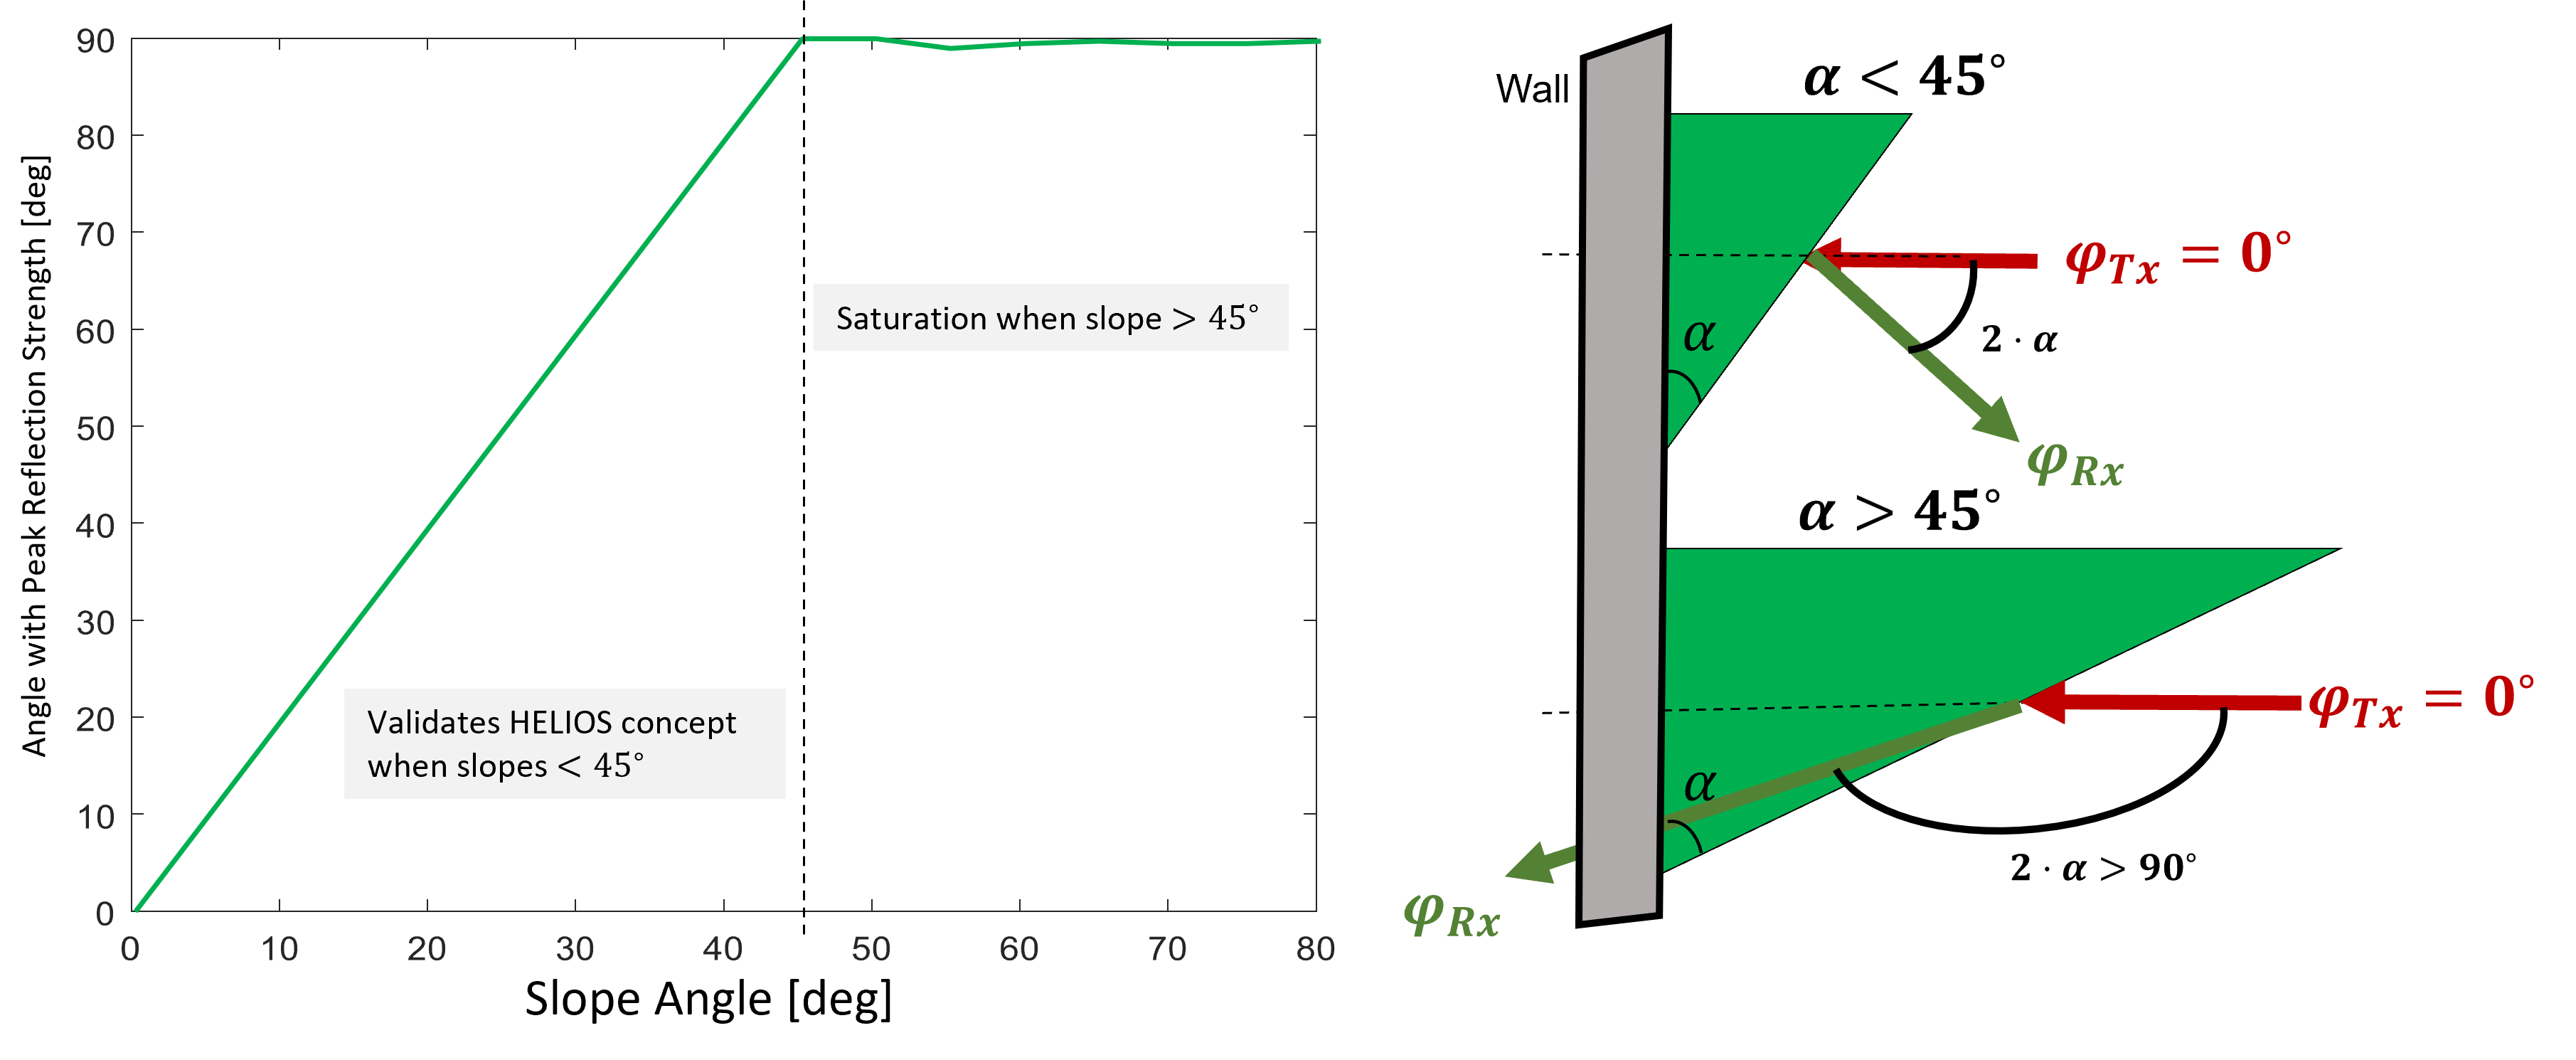
\includegraphics[width=0.93\linewidth]{images/Section 3 Images/Saturation}
	\caption{Assessment of the peak reflection angle given $\varphi_{Tx}=\theta_{Tx}=0^\circ$ and different module slopes. We observe that reflection angle $\varphi_{Rx} = -\varphi_{Tx} + 2\cdot \alpha$ and we note that the saturation for slopes $< \num{45}^\circ$ is misleading as this depends on the angle of arrival of the incident wave and, in particular, is caused by the maximum reflection angle being outside the specified observation angle range for the simulation. This is because the energy is reflected behind the reflector as sketched on the right side.}
	\label{fig:saturation}
\end{figure}
\subsection{Effect of Different Reflector Sizes} \label{Variation of Element Size}
We now make a complementary investigation of the impact of the HELIOS element footprint dimensions $a$ and $b$ with $a=b$ in the range from \num{1} to \SI{90}{\centi\meter}.

\begin{figure}[tb]
	\centering
	\subfloat[Azimuth angle variation at the reflector for various reflector sizes, plotted against gain in \si{\decibel} at \SI{28}{\giga\hertz} frequency with slope angle $\alpha=\num{22.5}^\circ$ with $\theta_{Rx}=0^\circ$. Notably, the beams become narrower as the reflector size increases.]{
	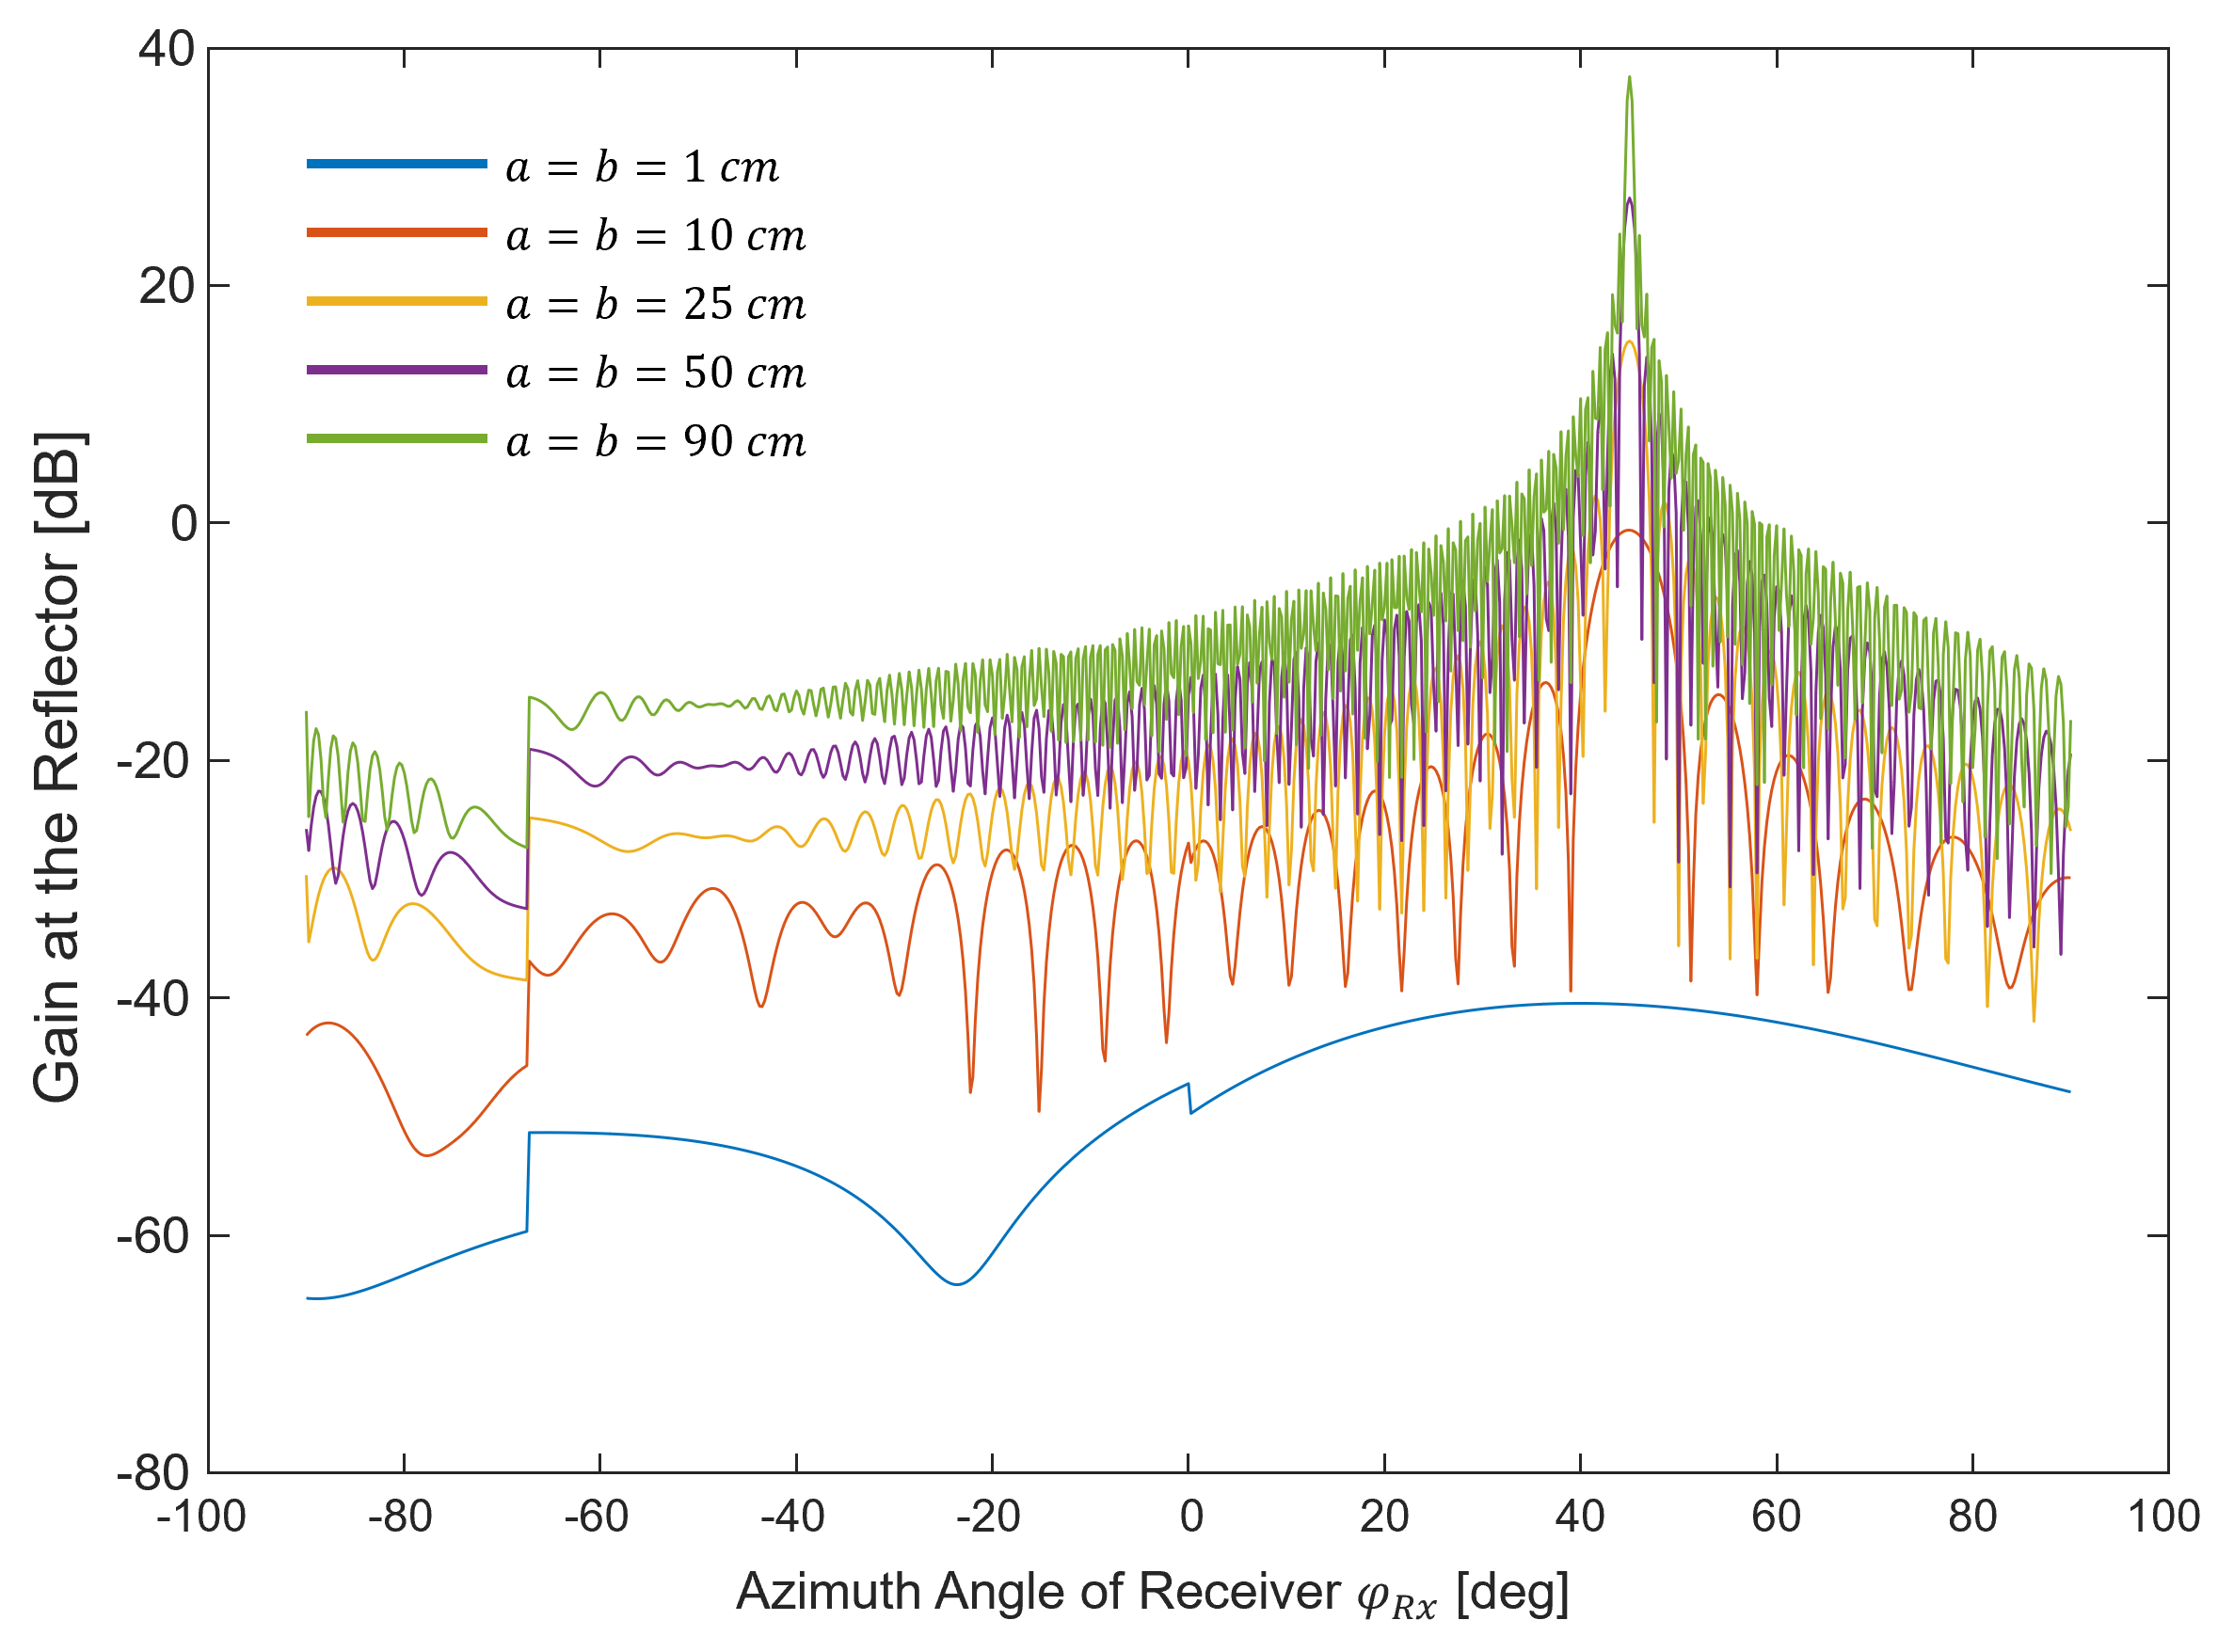
\includegraphics[width=0.5\linewidth]{images/Section 3 Images/Reflector_length_2}
		\label{fig:rl3}
	}
	\hfill
	\subfloat[Behavior of HELIOS module for varying reflector size $a$ and $b$ when plotted against peak gain in \si{\decibel}. A notable increase in gain by \SI{12}{\decibel} is observed when the reflector size is doubled.]{
	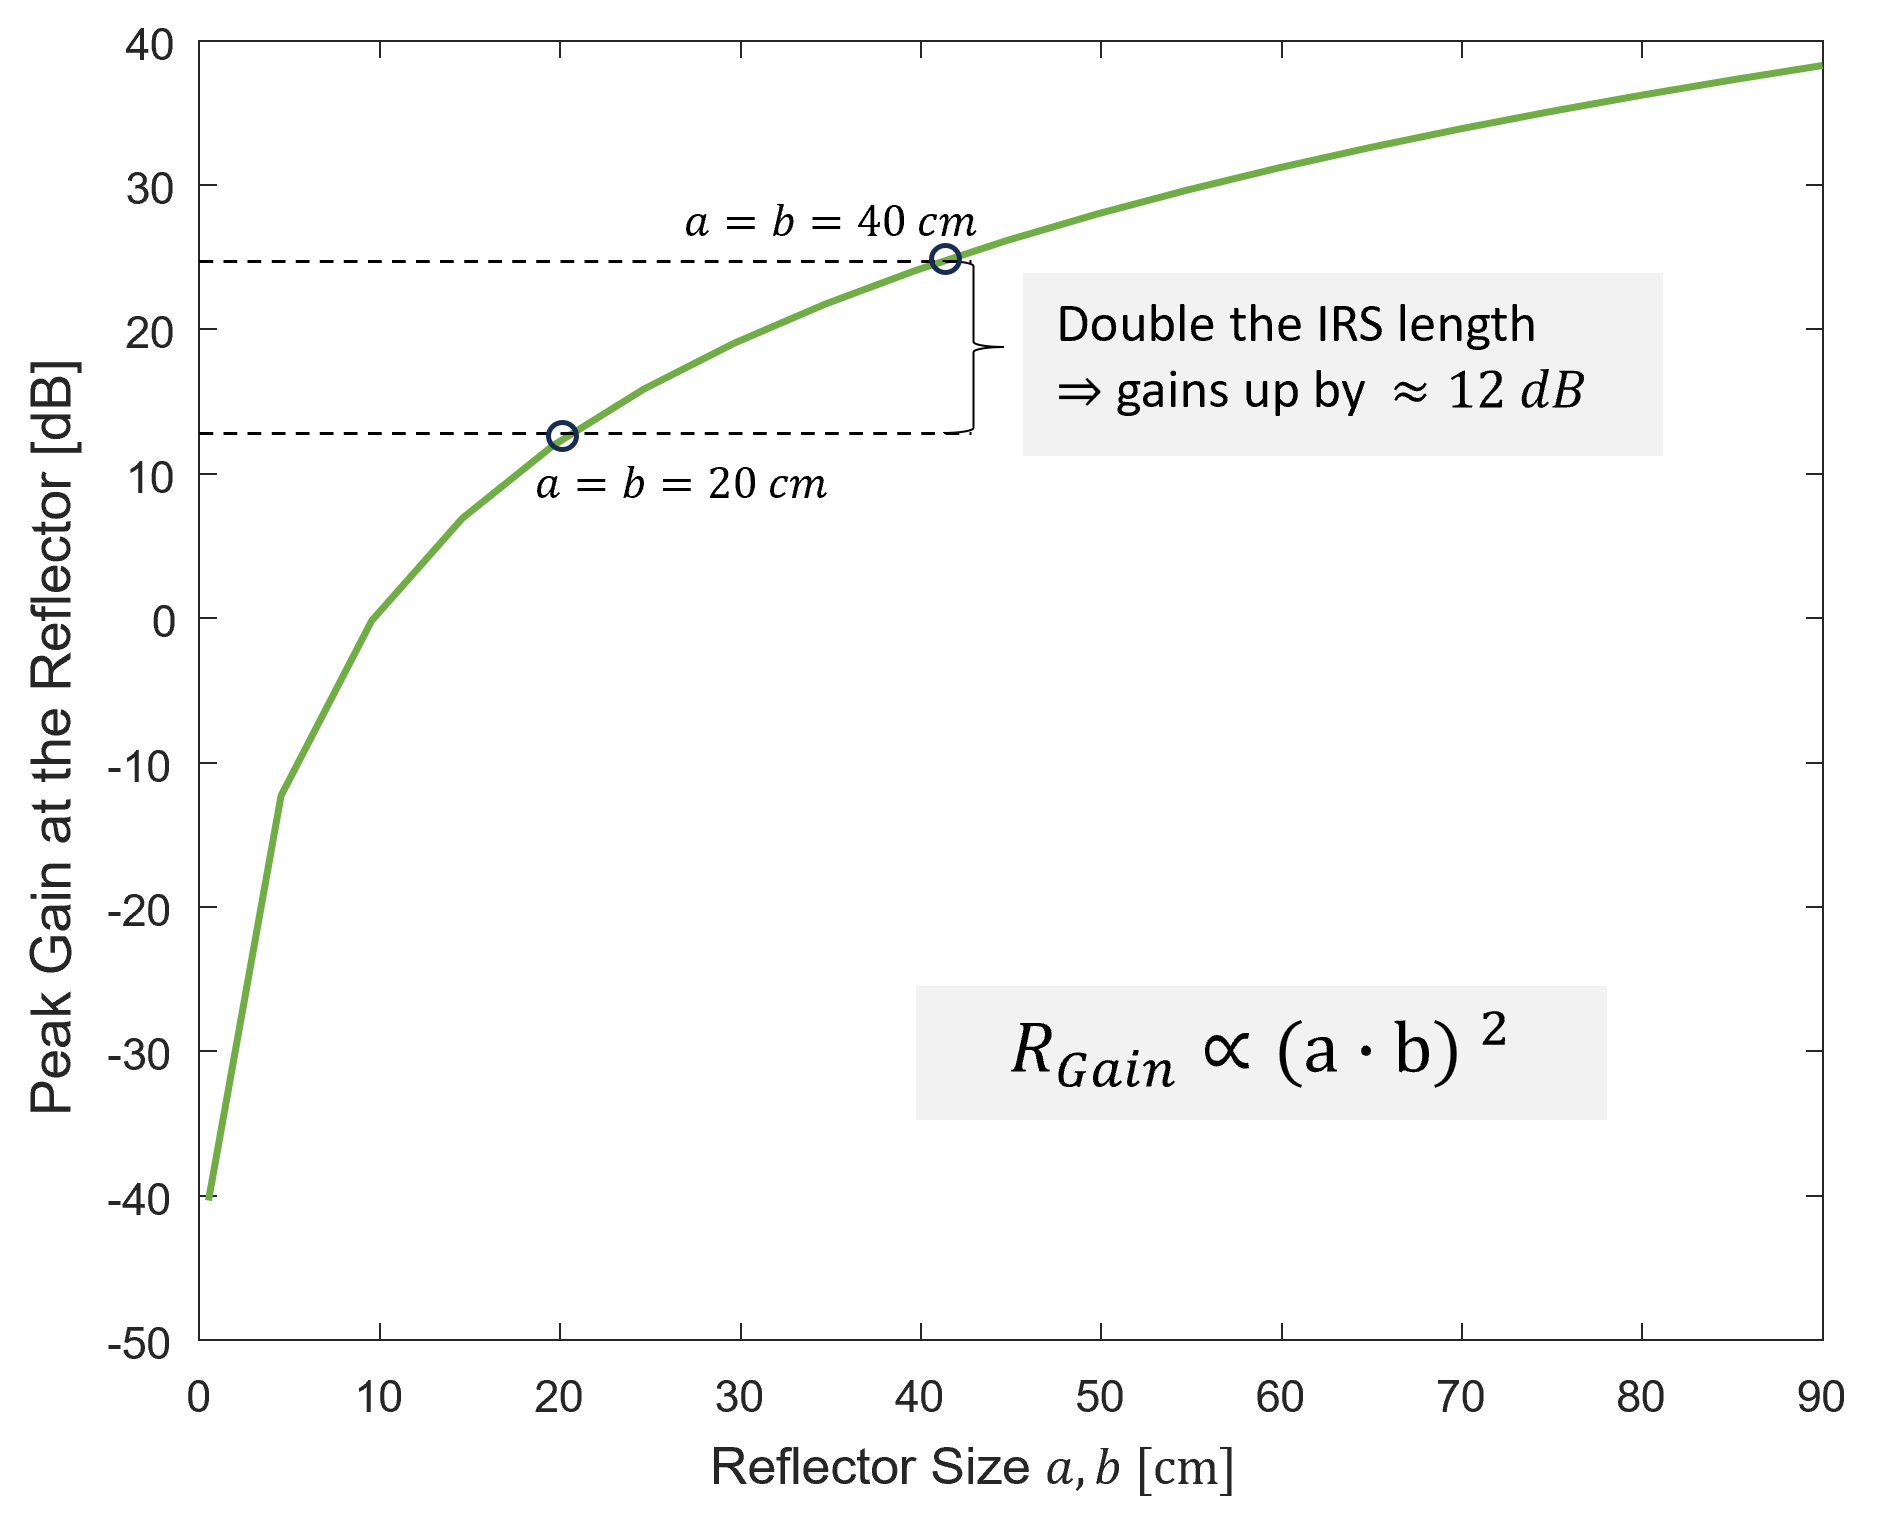
\includegraphics[width=0.45\linewidth]{images/Section 3 Images/Reflector_length}
		\label{fig:rl1}
	}
	\caption[Illustration of the impact of the variations in reflector sizes of HELIOS module on the beam pattern and peak gain at the reflector as the size increases.]{Illustration of the impact of the variations in reflector sizes of HELIOS module on the beam pattern and peak gain at the reflector as the size increases.}
	\label{}
\end{figure}
%\begin{figure}[H]
%	\centering
%	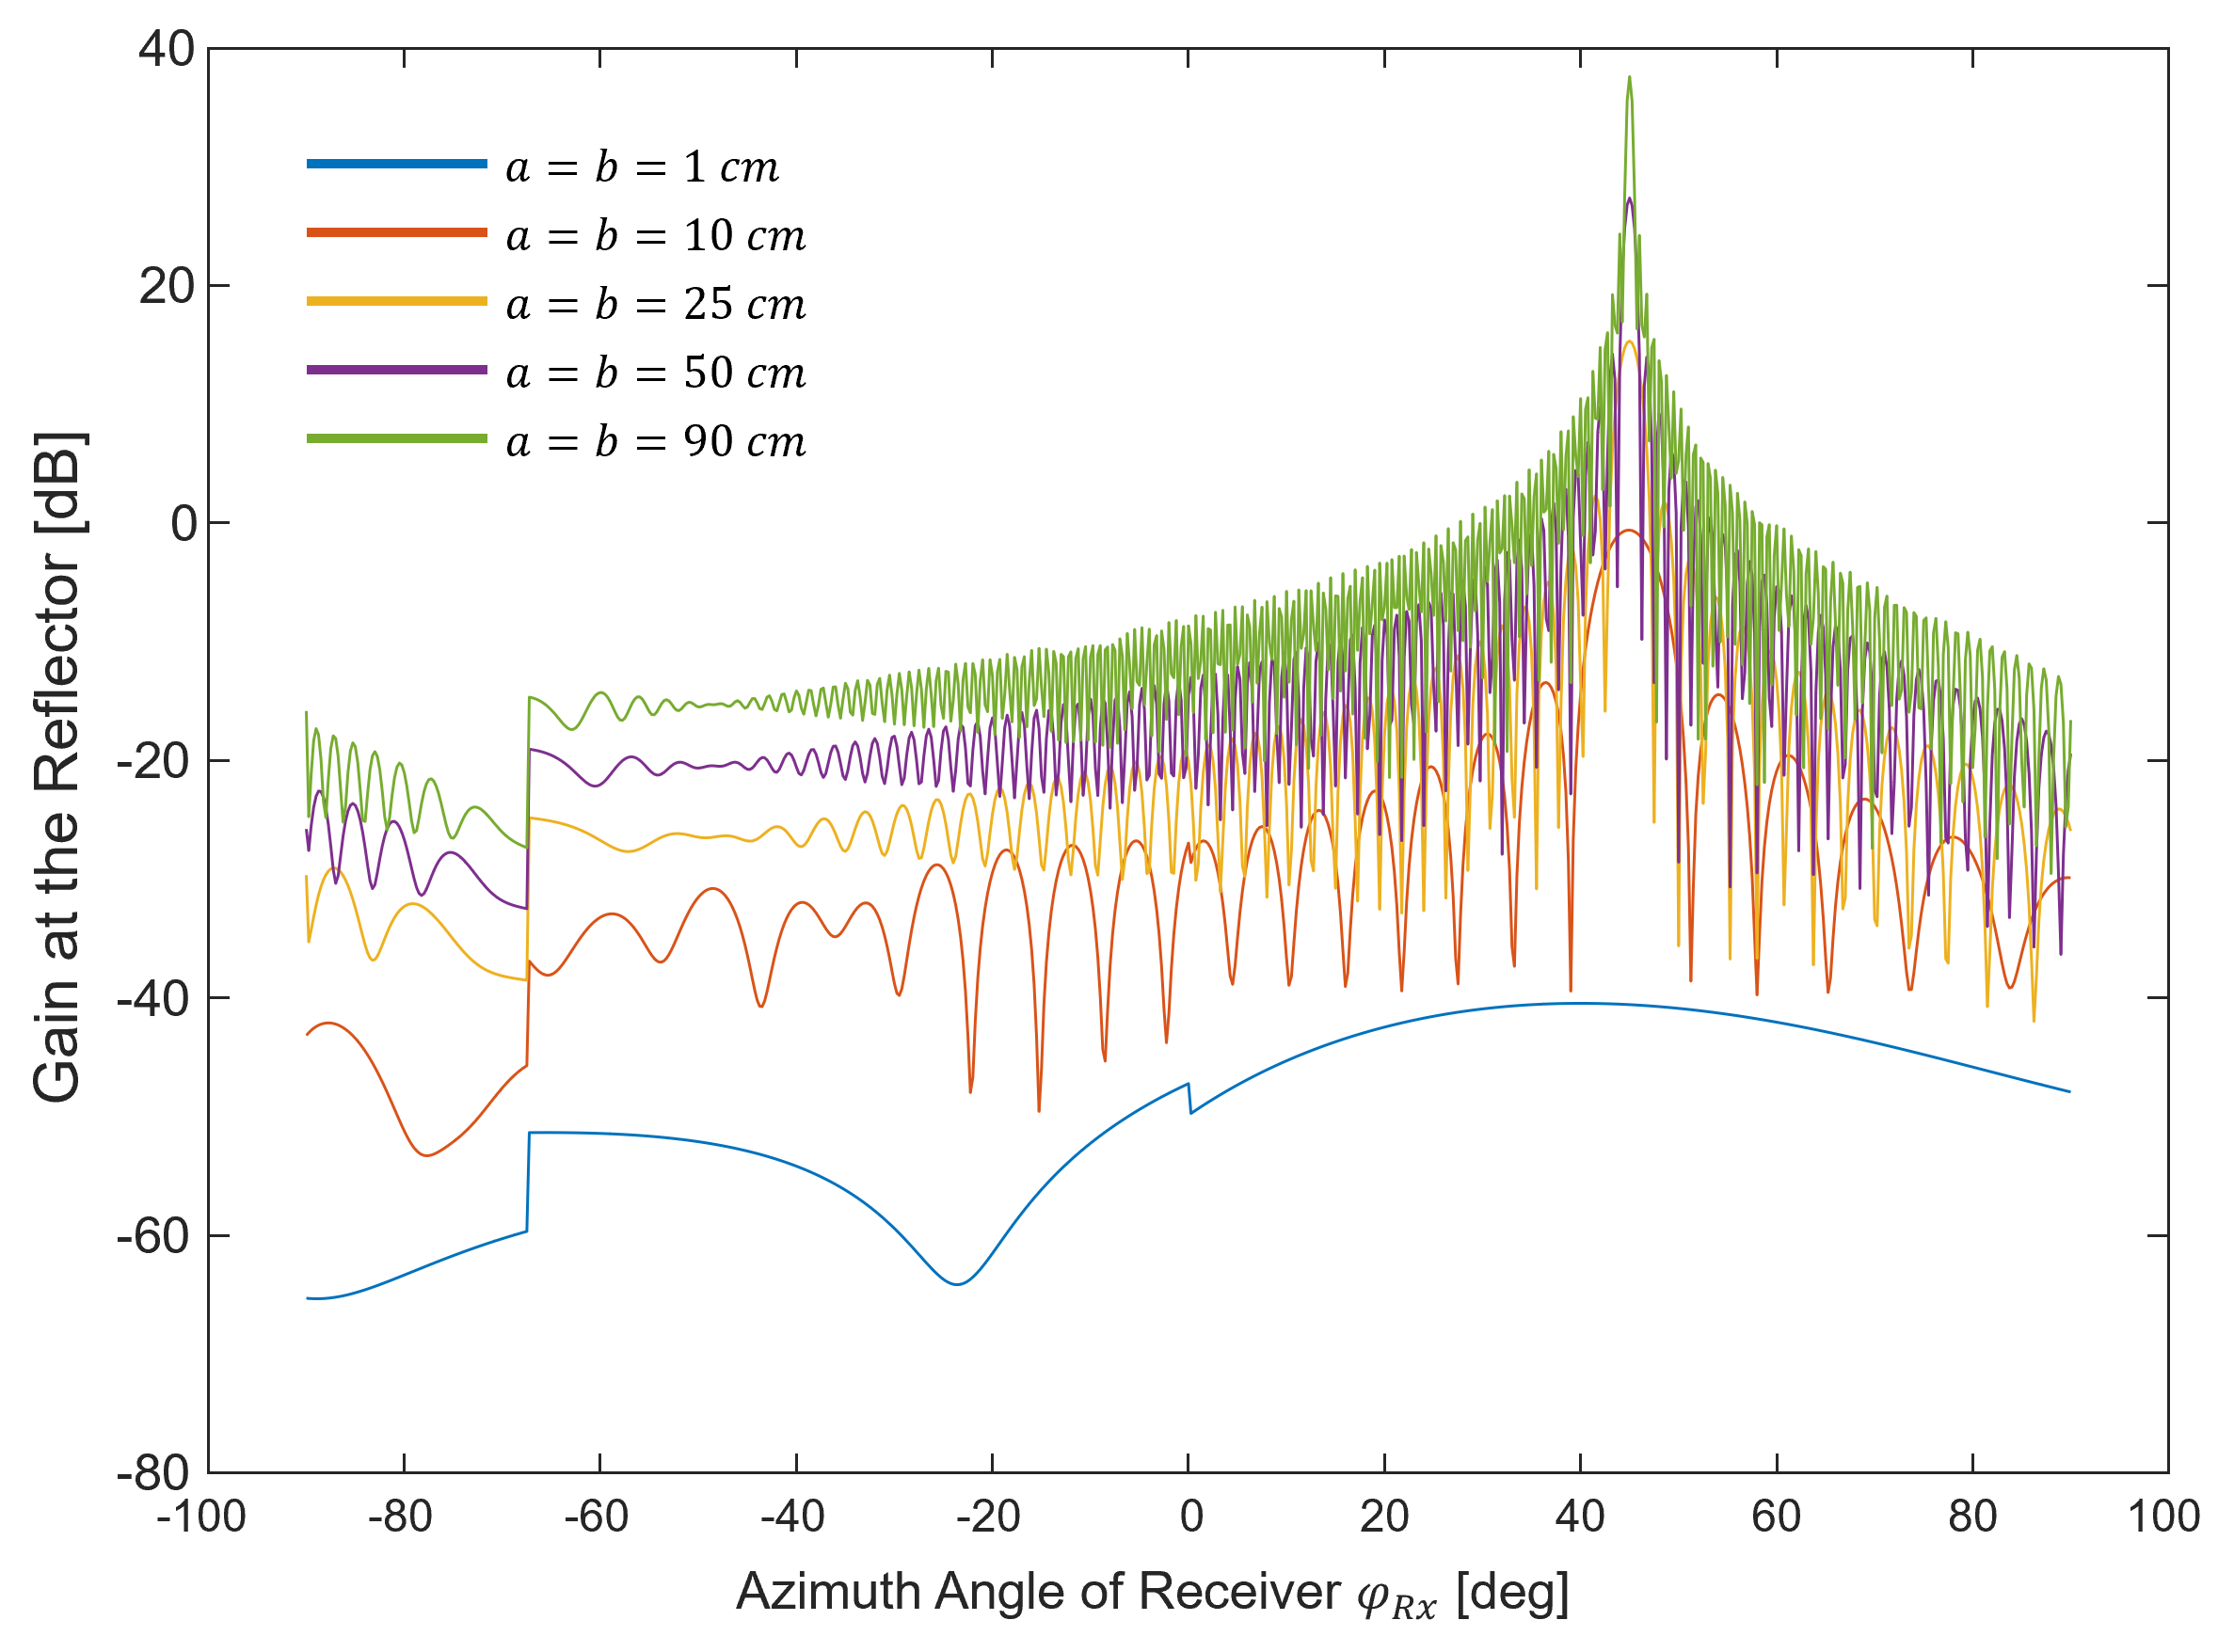
\includegraphics[width=0.8\linewidth]{images/Section 3 Images/Reflector_length_2}
%	\caption{Azimuth angle variation at the reflector for various reflector sizes, plotted against gain in \si{\decibel}.}
%	\label{fig:rl3}
%\end{figure}
%\begin{figure}[H]
%	\centering
%	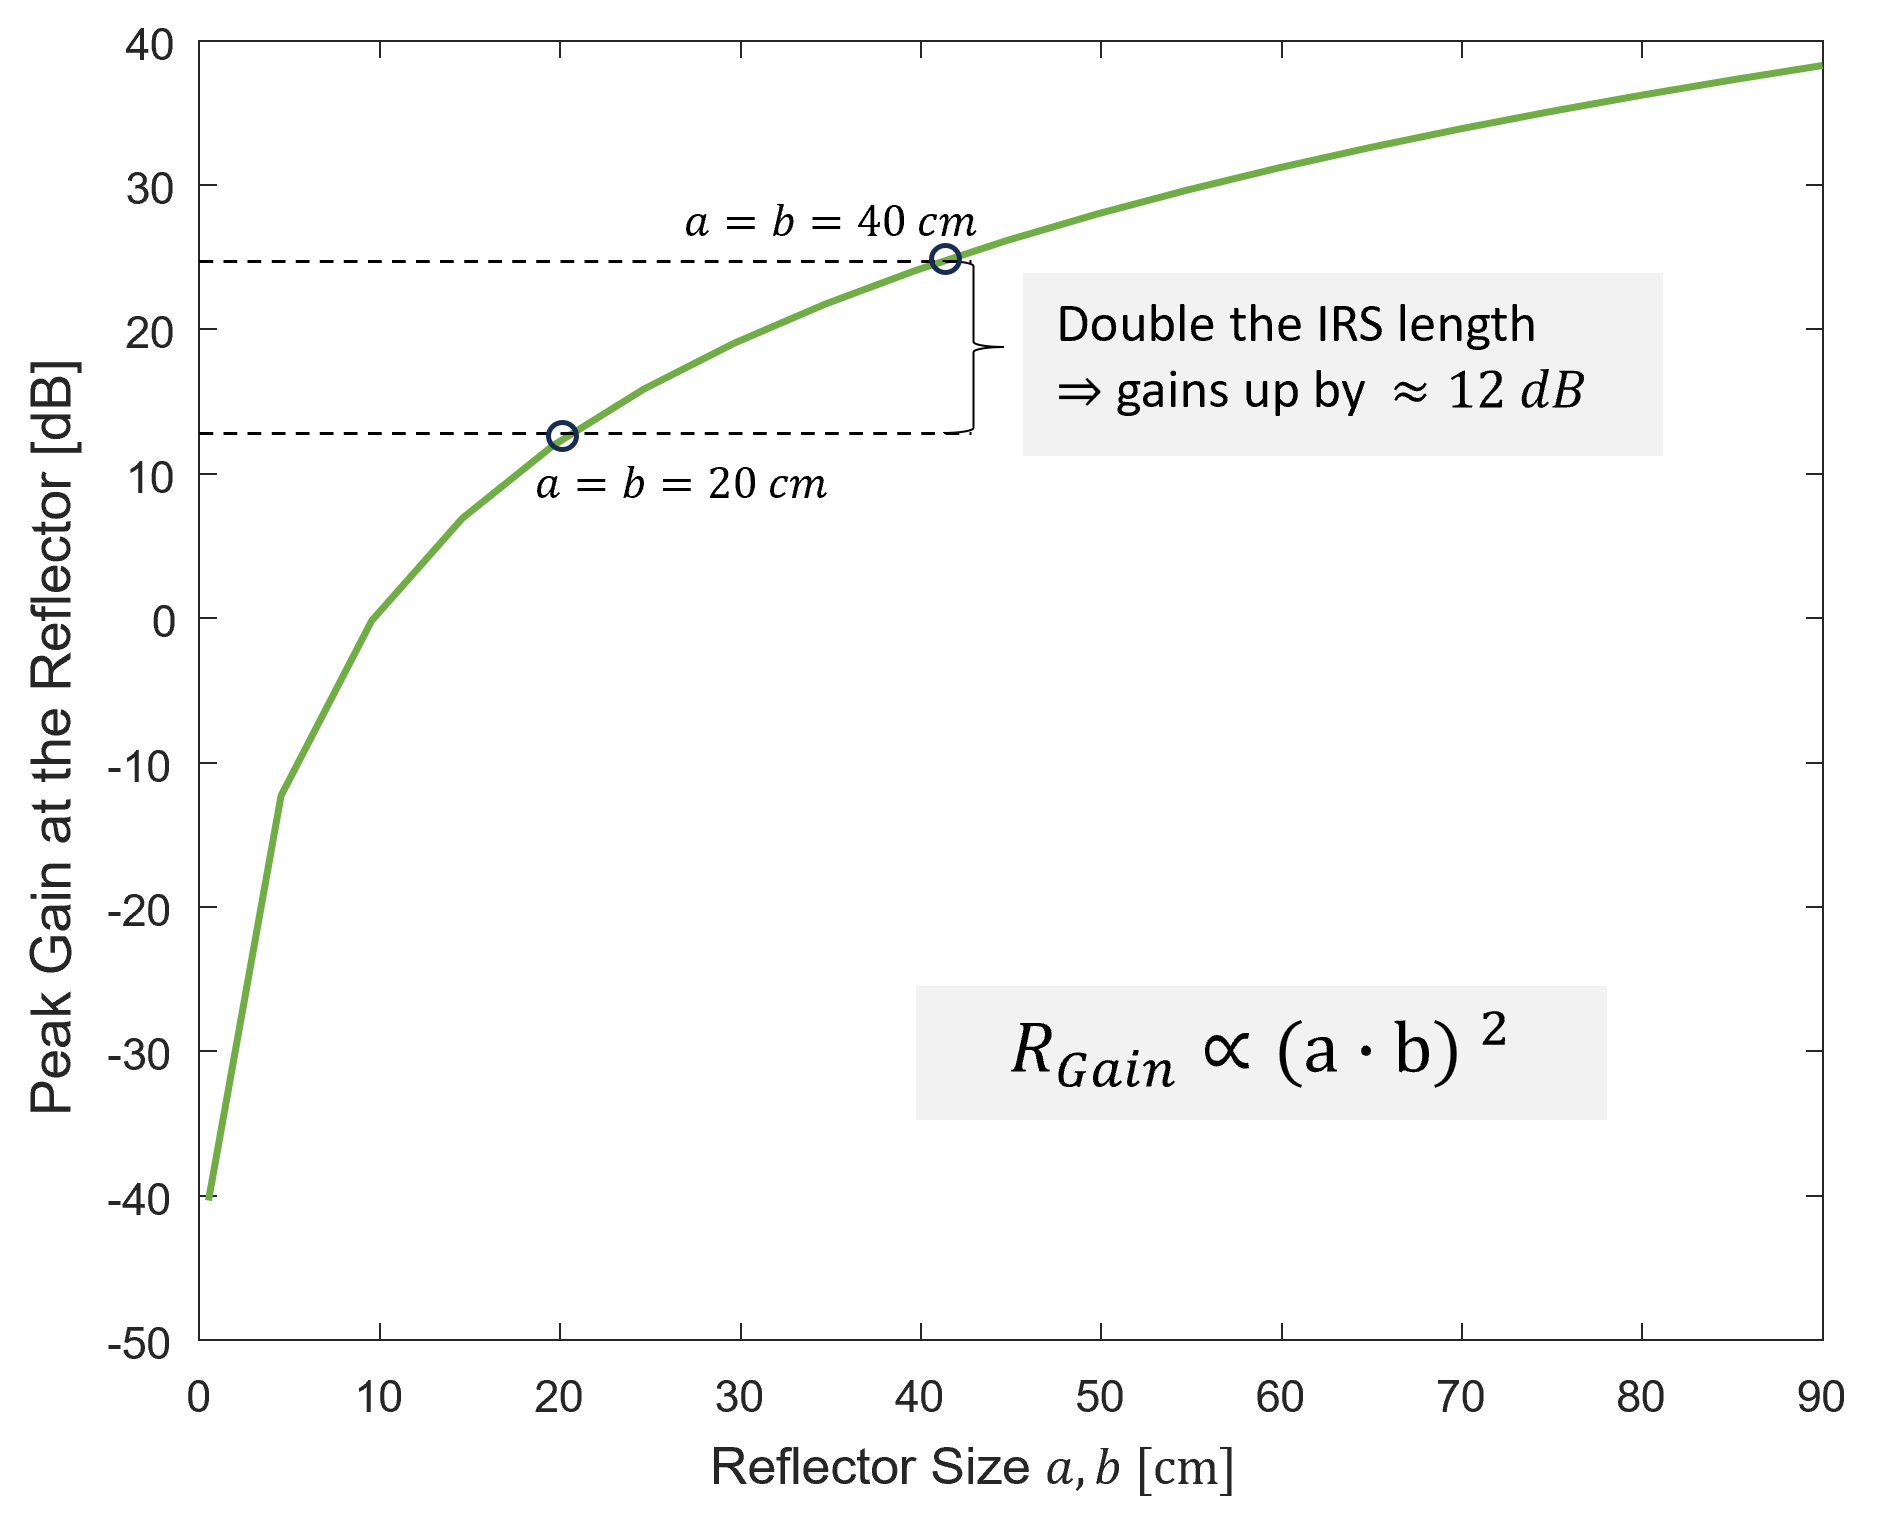
\includegraphics[width=1.0\linewidth]{images/Section 3 Images/Reflector_length}
%	\caption{Behavior of HELIOS module for varying reflector size when plotted against gain in \si{\decibel} for different orientations. Linear scale behavior of HELIOS module for varying reflector size which validates the gain proportionality with reflector dimensions.}
%	\label{fig:rl1}
%\end{figure}
The simulation results in \Cref{fig:rl3} illustrate that larger reflecting surfaces produce a higher gain. Moreover, with increasing size, the main lobe also becomes more narrow such that energy is reflected in a more concentrated fashion. The results in \Cref{fig:rl1} match the analytical modeling carried out in \Cref{coordinate systems} in regards to the maximal gain which scales with $(a\cdot b)^2$, cf. gain increase by \SI{40}{\decibel} when increasing the surface area by a \num{100} from $a=b=\SI{1}{\centi\meter}$ to $a=b=\SI{50}{\centi\meter}$. As observed from the same figure, as we double the size of the reflector from $a=b=\SI{20}{\centi\meter}$ to $a=b=\SI{40}{\centi\meter}$, the peak gain increases by almost \SI{12}{\decibel}. This result confirms that reflector size is a key metric to be tuned to attain the necessary power gains for mmWave beyond LOS connectivity.
\subsection{Impact of Reflecting Surface Material} \label{Impact of Material Conductivity}
Lastly, we study the impact of material properties on the reflection behavior. In the first part, we consider seven different real materials. Thereafter, we consider the impact of the material conductivity directly. 
\begin{table}[tb] % H -> dieses objekt wird genau da wo der code steht festgenagelt
			\caption{Properties of different materials in terms of conductivity and relative permittivity.}
		\footnotesize
	\label{Conductivity table}
	\centering
	\begin{tabular}{c|c|c}
		\textbf{Materials} & \textbf{Conductivity} (\si{\siemens/\meter}) & \textbf{Relative Permittivity} \\
		\hline
		Copper & 58,000,000 & 1 \\
		\hline
		FR4 & 0 & 4.4 \\
		\hline
		Glass & 0 & 5.5 \\
		\hline
		Perfect Electric Conductor & 1e+30 & 1 \\
		\hline
		Tantalum & 6,300,000 & 1 \\
		\hline
		Stainless Steel & 1,100,000 & 1 \\
		\hline
		Rubber & 0 & 3.0
	\end{tabular}
\end{table}
First, we consider the maximum gain by HELIOS modules based on the seven materials given in \Cref{Conductivity table}. The maximum gains observed in \Cref{fig:conductivity1} underline that high material conductivity results in stronger reflections. As a result, high gains can only be realized by using large reflecting surfaces (cf. \Cref{Variation of Element Size}) and correct slope angles (cf. \Cref{Variation of Slope Angle}) in combination with a suitable reflecting surface material such as copper. Since the four materials yielding high gains have very similar peak gains, we now do a sensitivity analysis for a wide range of conductivity values using an artificial material, copper, and only alter the conductivity parameter as needed.

The sweep range is between $\num{0}$ to 10,000 $\si{\siemens/\meter}$ and thus exceeds the conductivity of glass, FR4, and rubber by far. However, the value is much smaller than that of, e.g., copper. The findings, as shown in \Cref{fig:conductivity2}, underline that the reflection gain does indeed depend nearly linearly on the material conductivity, as underlined by the linear regression curve (red). This behavior matches the IRS model dependence on parameter $\Gamma$ in \Cref{coordinate systems}. 
 
The potential to use these materials to improve the performance of our HELIOS reflector modules in practical applications is highlighted by the intriguing consistency between the behavior of high conductivity materials and the IRS models. We are better able to design and deploy our modules for practical and efficient use if we are aware of these subtle interactions between materials and their conductivity values.

\begin{figure}[H]
	\centering
	\subfloat[Effect of different materials on HELIOS module when plotted against the gain in \si{\decibel}. Parameters: $\alpha=22.5^\circ$, $\beta=0^\circ$, $a=b= \num{50} \cdot \lambda$ with incident wave $\varphi_{Tx}=\theta_{Tx}=0^\circ$ at \SI{28}{\giga\hertz} frequency.]{
		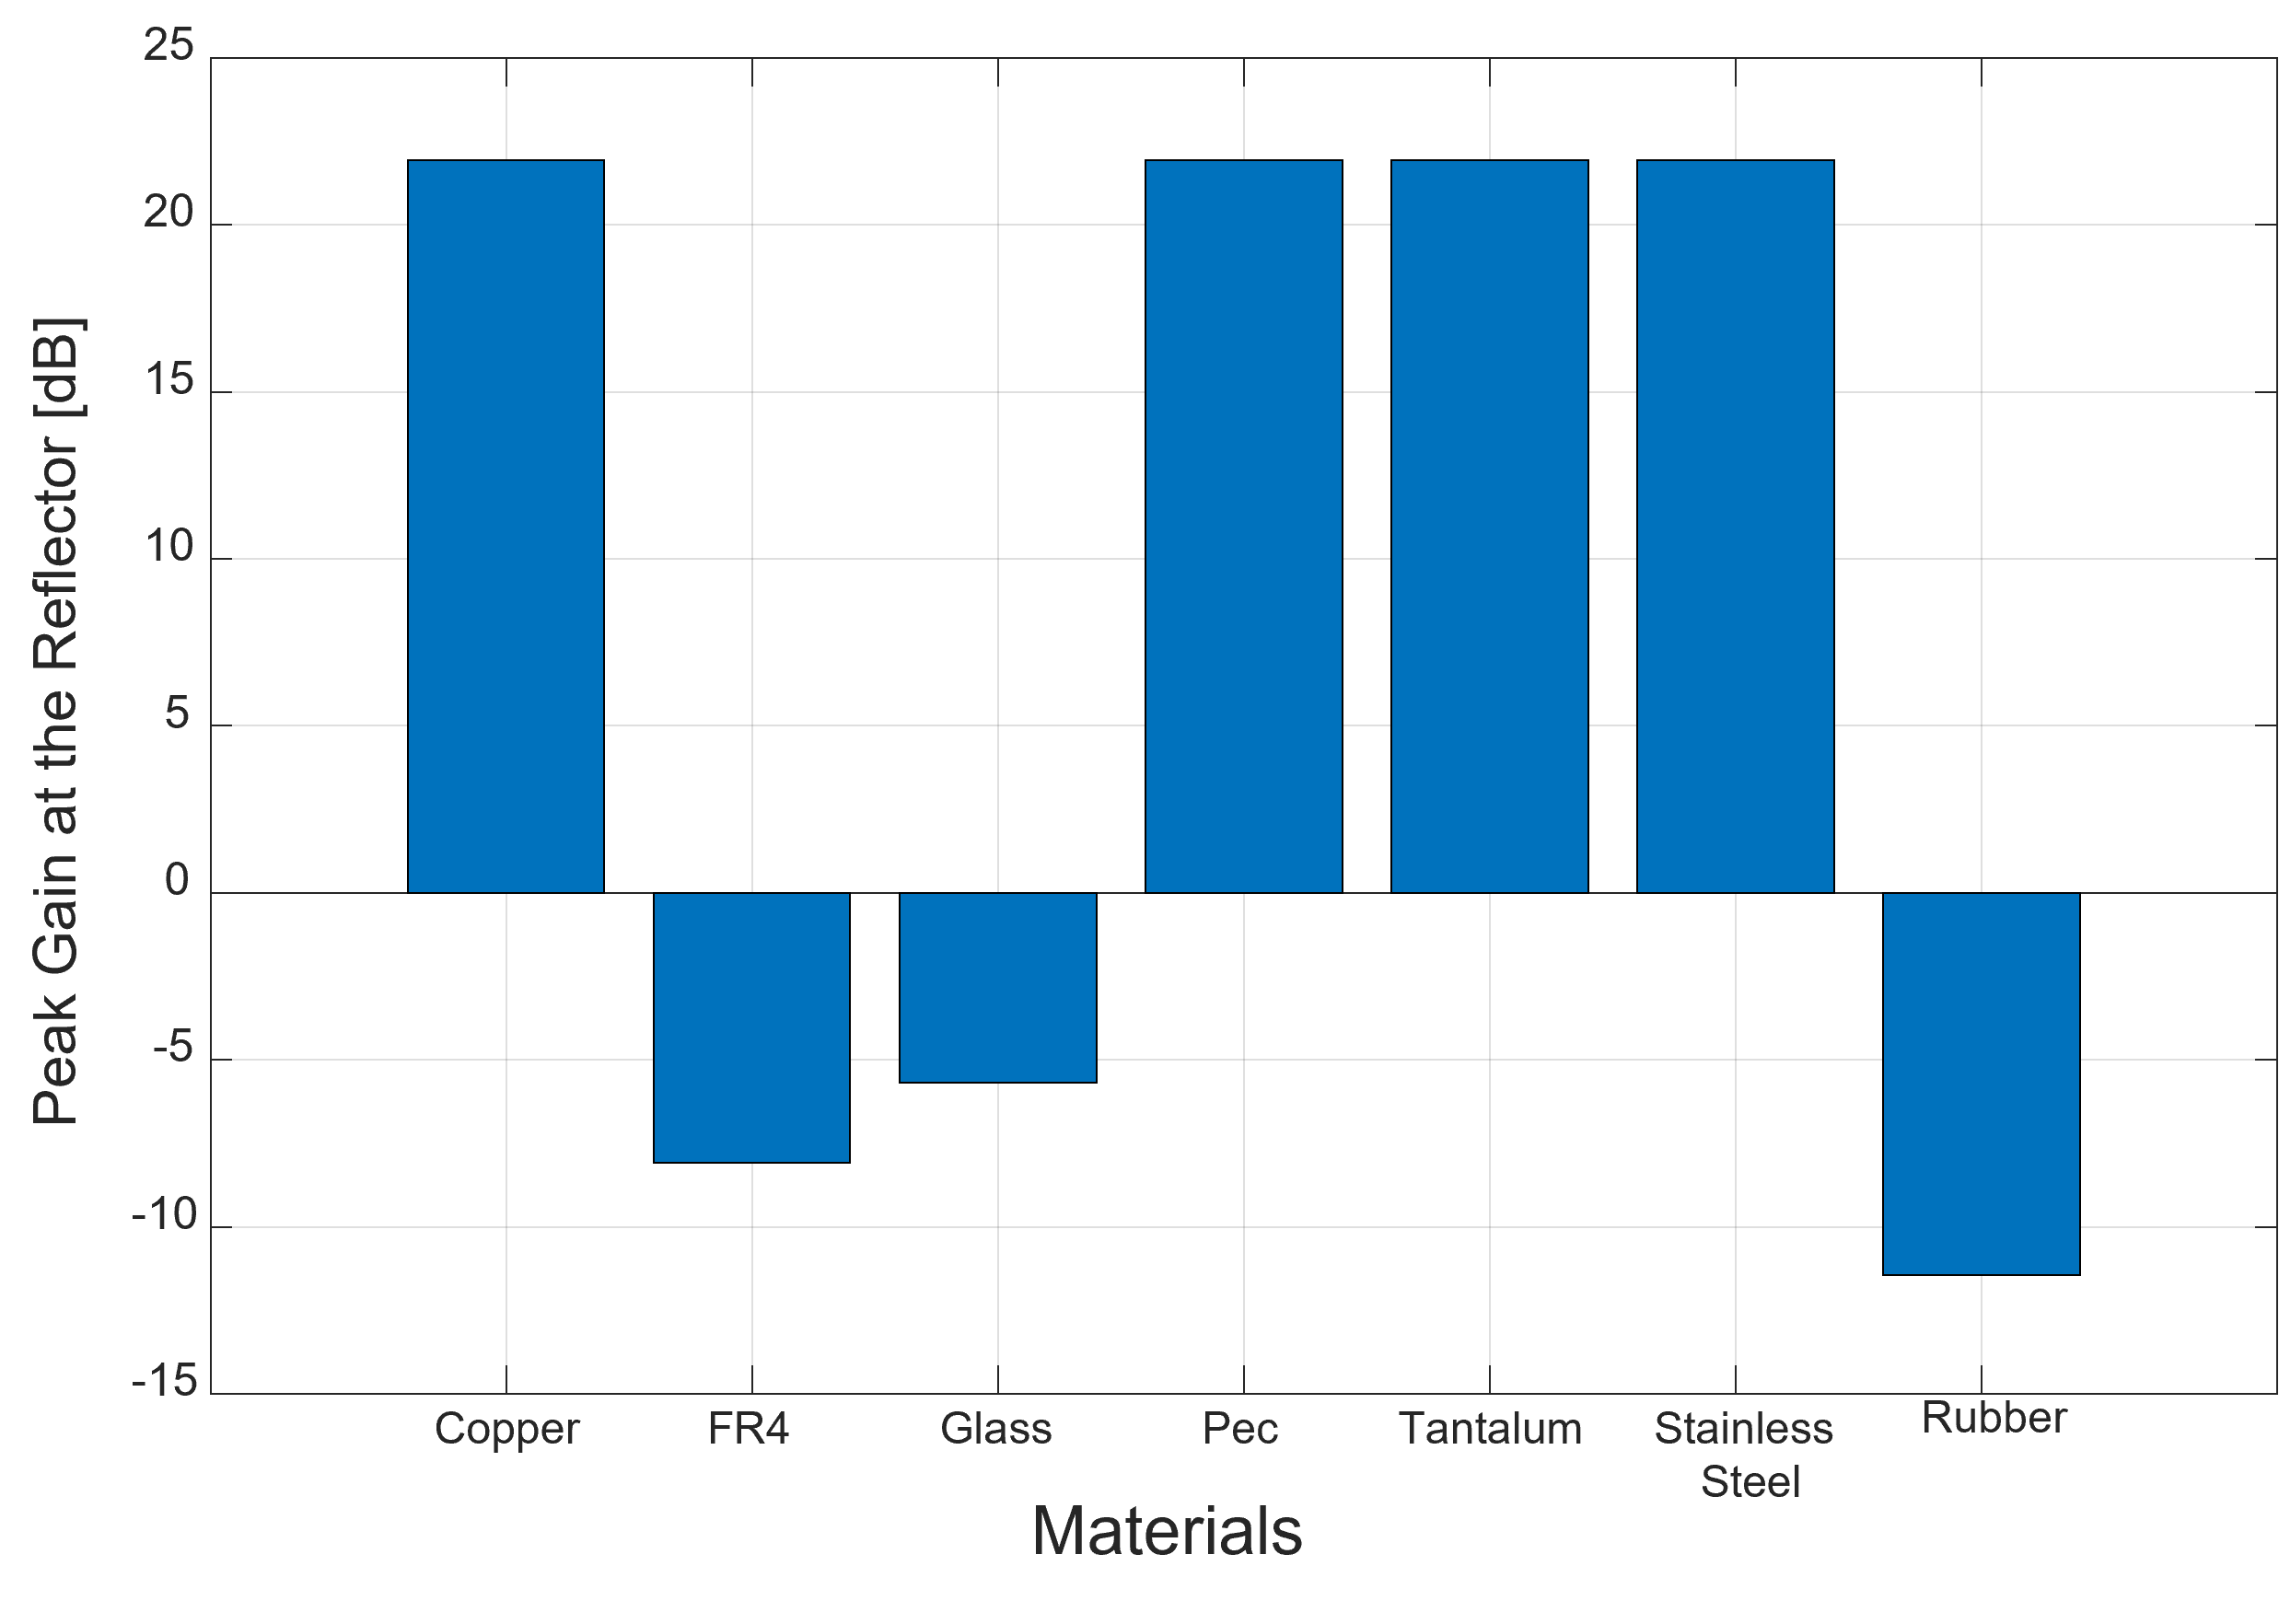
\includegraphics[width=0.5\linewidth]{images/Section 3 Images/Material1}
		\label{fig:conductivity1}
	}
	\hfill
	\subfloat[Peak reflection gains from simulations utilizing copper with modified conductivity as the base material of a HELIOS reflector module (blue). Linear regression curve (red) underlines roughly linear dependence on conductivity in the considered range.]{
		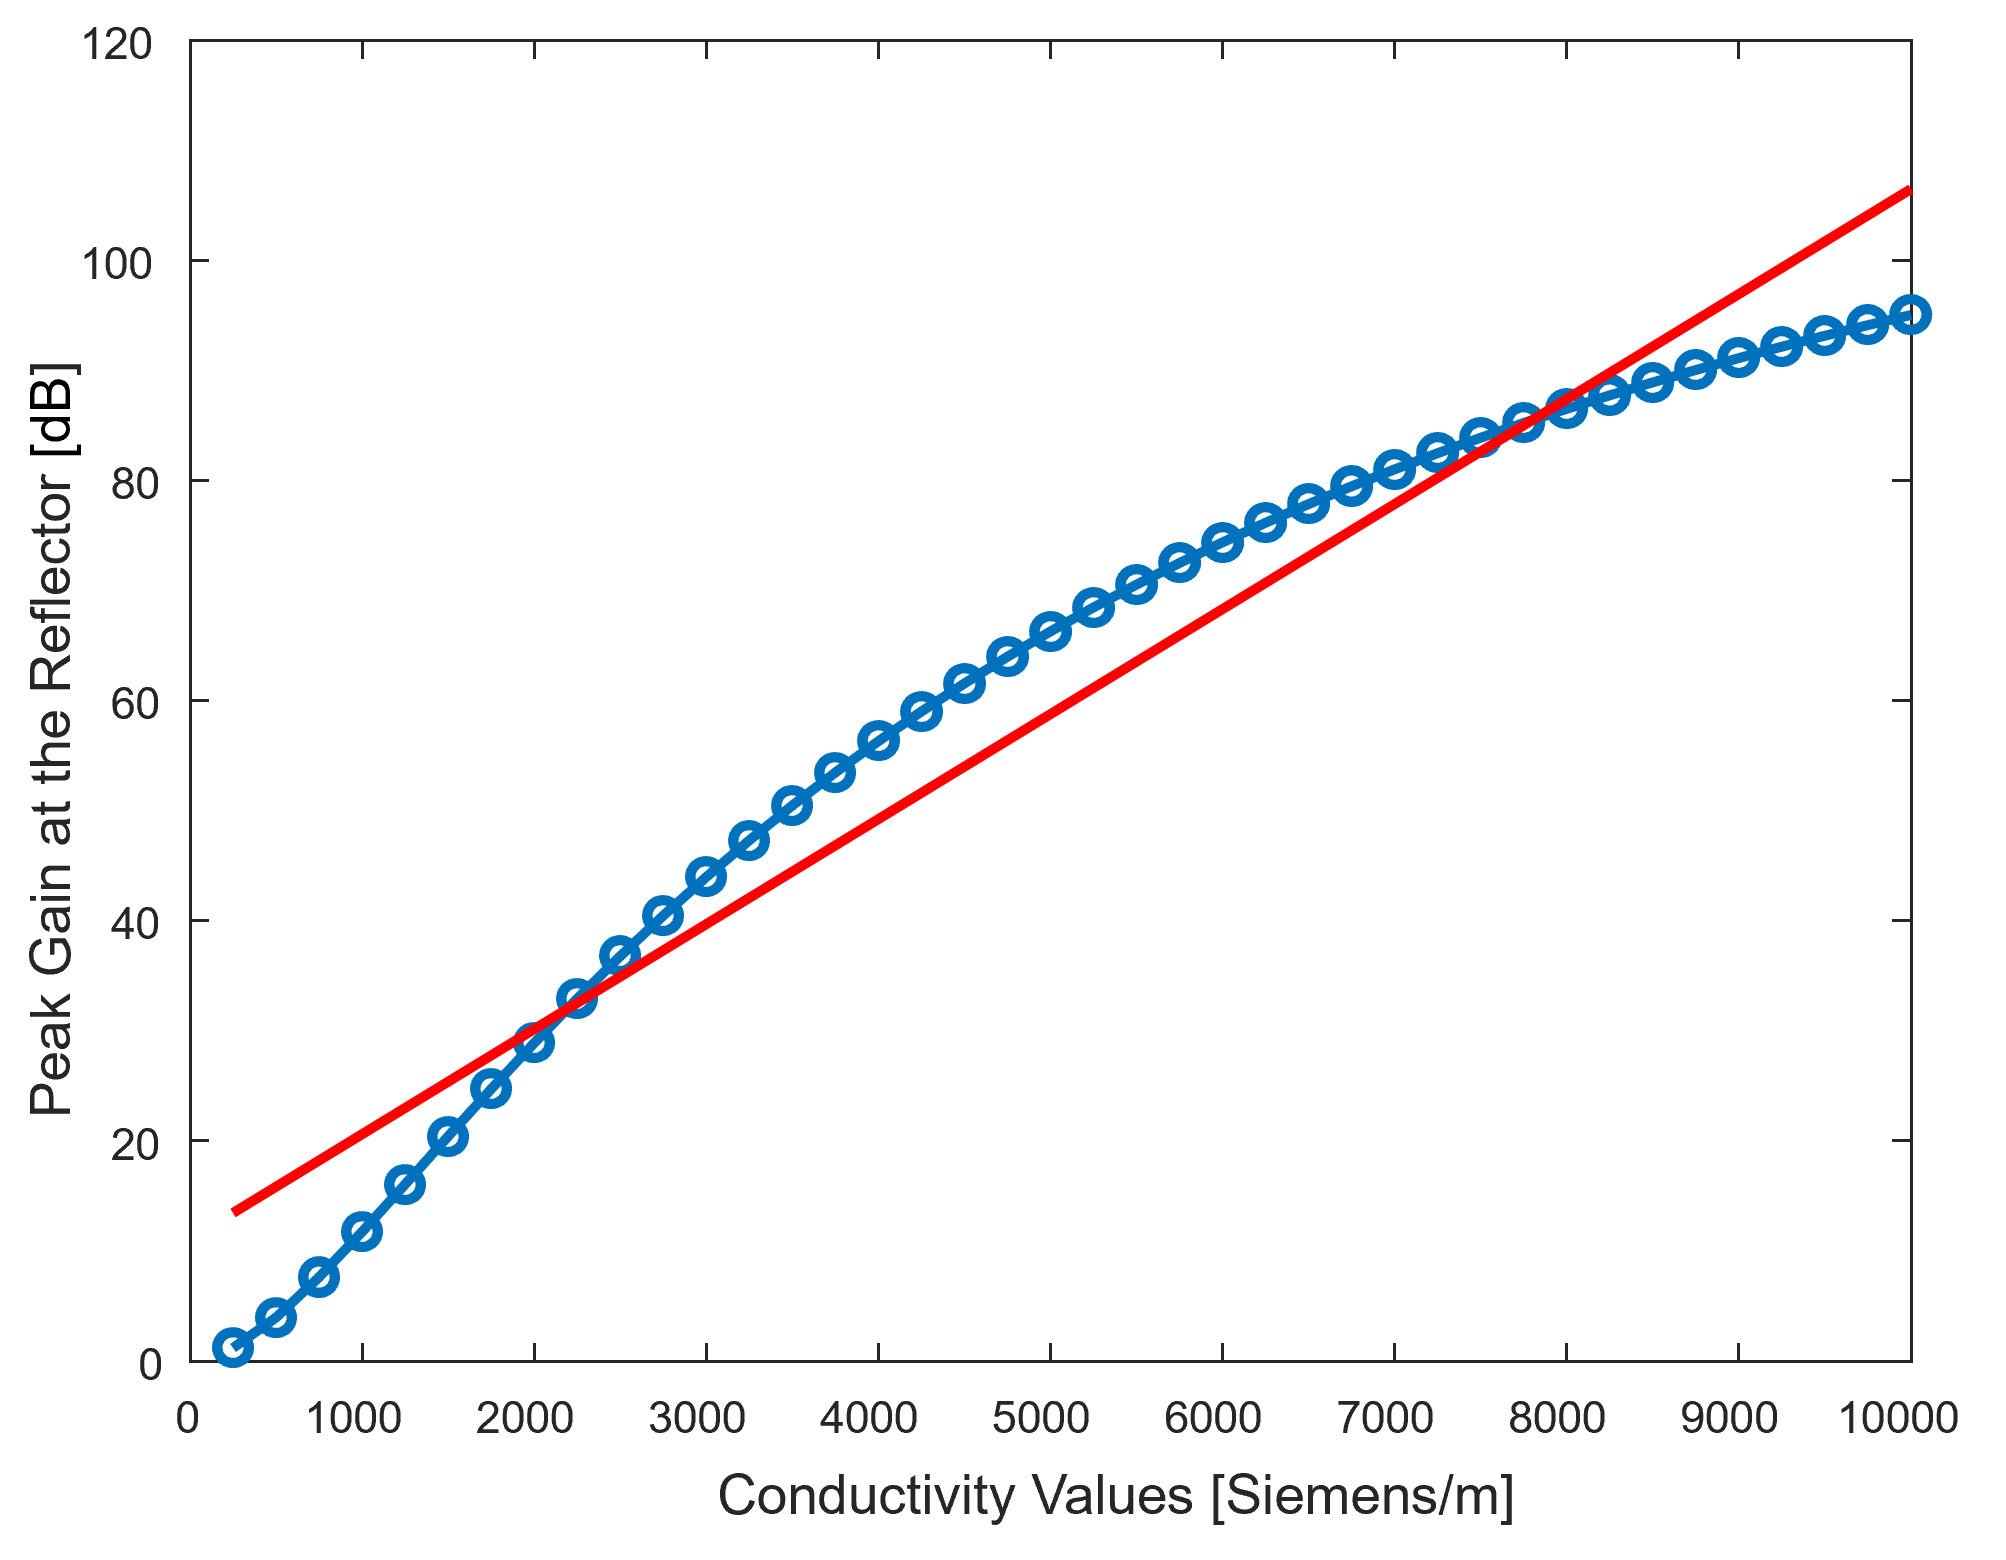
\includegraphics[width=0.45\linewidth]{images/Section 3 Images/conductivity2}
		\label{fig:conductivity2}
	}
	\caption[The influence of a reflecting surface on gain for various materials based on their conductivity and relative permittivity.]{The influence of a reflecting surface on gain for various materials based on their conductivity and relative permittivity.}
	\label{}
\end{figure}
\section{Analytical Modeling of HELIOS Modules} \label{Analytical Modeling of HELIOS Modules}
This section makes the crucial first step in developing the analytical model for the reflection characteristics of HELIOS reflectors by first considering only an individual HELIOS module. This is in coordination with the simulation results in \Cref{Simulative Analyses of HELIOS Reflector Modules} and the analytical models for IRSs in \Cref{coordinate systems}. For this purpose, we introduce the notion of the radar cross section in \Cref{Radar-Cross-Section and Radar Equation} which was already previously set to be the solution type of the EM wave simulator, cf. \Cref{sec:Simulation Methodology}. In \Cref{Transfer and Adaption of Model to HELIOS Modules}, we will discuss how RCS can be analytically adapted to HELIOS reflectors by also doing assessments with the EM simulation results in \Cref{Assessment of Differences between Simulations and Analytical Model}.
\subsection{Bistatic Radar Cross Section} \label{Radar-Cross-Section and Radar Equation}
The \ac{RCS} concept is a crucial tool in this thesis. It allows us to characterize how objects, in this case, our HELIOS model, interact with electromagnetic waves. \ac{RCS} is a fundamental concept in radar engineering and electromagnetic scattering \cite{Balanis, Kerr1989PropagationOS}. When an object is illuminated by electromagnetic waves, usually carrying radar signals, the \ac{RCS} describes the scattered power per unit solid angle from the object. It offers information about how "visible" an object is to radar systems. By describing the RCS of HELIOS reflectors in this thesis, our model may be used to estimate how it will appear to wireless systems such as 5G/6G.

The radar equation below shows how the RCS $\sigma_{Meta}$ can be considered in a channel model \cite{RCS1}. But first, it needs to be determined as follows. The formula in \Cref{Eq:RCS_rtendsto inf} gives the common definition of the RCS, which is written as the limit of the distance $r$ to infinity.
\begin{equation} \label{Eq:RCS_rtendsto inf}
	\sigma_{Meta}= \lim_{r\to\infty} 4 \pi r^2 \frac{|E_{Rx}|^2}{|E_{Tx}|^2} ,
\end{equation}
where $\sigma_{Meta}$ \footnote{$\sigma_{Meta}$ has an additional unit of $\si{\meter}^2$ and for simplicity, we mention \si{\decibel} instead of \si{\decibel}sm.} \footnote{The term "Gain" refers to the RCS, as elucidated in \Cref{Analytical Modeling of HELIOS Modules}, throughout this work.} is the RCS for the metasurface, and $E_{Rx}$ and $E_{Tx}$ are the far-field reflected and incident electric field intensities, respectively. As such, it is the ratio of incident and reflected wave in the infinite far-field. Fixing the direction of the incident wave and varying the considered reflection angle, the RCS becomes a multivariate reflection pattern similar to an antenna pattern \cite{RCS_1, RCS_2}. \Cref{Table:standard_sigma_values} below provides the standard RCS values that are usually encountered in the communication link. A non-zero $\sigma_{Meta}$ becomes relevant to account for real-world situations, including the existence of obstructions like a car within the communication channel. On the other side of the coin, a car typically comes with an RCS of \SI{20}{\decibel}sm, which is larger than the \SI{0}{\decibel}sm of a person, according to \Cref{Table:standard_sigma_values}.

\begin{table}[tb] % H -> dieses objekt wird genau da wo der code steht festgenagelt
	\caption{Standard RCS values which are commonly observed \cite{RCS_meta, RCS_meta2}.}
	\footnotesize
	\label{Table:standard_sigma_values}
	\centering
	\begin{tabular}{c|c}
		\textbf{Object} & \textbf{$\sigma_{Meta}$ [dBm]} \\
		\hline
		Man & \num{0}\\
		\hline
		Small bird & \num{-20}\\
		\hline
		Car & \num{20}\\
		\hline
		Large commercial airplane  & \num{20}\\
		\hline
		Small fighter plane  & \num{3}\\
	\end{tabular}
\end{table}
The application of bistatic RCS analysis necessitates a thorough comprehension of important variables, especially the angles of the incidence and departure which are crucial for evaluating randomly shaped scattering objects, in literature also referred to as radar targets \cite{Balanis, RCS2}.

The main reflection angle and magnitude of the scattered signal are strongly dependent on the angle of the incident and the shape of the object. To fully understand bistatic RCS one must first study the monostatic RCS, which is concerned with calculating the power reflected to the transmitting node \cite{RCS_3}. When the transmitter and receiver are in the same place, monostatic RCS measures the amount of power that a scatterer reflects to the transmitting node, hence indicating the visibility of an object. Conversely, bistatic RCS measures reflected power when the transmitter and receiver are at different sites. This latter case is thus more relevant for 5G/6G mmWave communications, although the monostatic RCS can be of interest for future 6G \ac{JCAS} use cases.
\subsection{Analytical Model for the Reflection of Planar Surfaces} \label{Analytical Model for the Reflection of Planar Surfaces}
In literature, one may find a formula for the bistatic RCS of a rectangular plate. It depends on the following parameters:
\begin{itemize}
	\item Plate dimensions and materials
	\item Carrier frequency
	\item Angles of incident and reflected wave
\end{itemize}
Taking into account the above-mentioned parameters, RCS formulas have been derived in literature \cite{Helios, Kerr1989PropagationOS, Balanis} as follows:
\begin{equation} \label{RCS_flatplate}
	\begin{aligned}
	\sigma_{plate} = 4 \cdot \pi \cdot \left( \frac{a \cdot b}{\lambda} \right)^2 \cdot \cos^2 \left( \theta_{Rx} \right) \cdot \sinc^2 \left( \frac{\pi \cdot b \cdot \left( \sin \left(\theta_{Rx} \right) \cdot \sin \left( \varphi_{Rx} \right) \pm \sin \left( \theta_{Tx} \right) \right) }{\lambda} \right) \\
			\begin{cases}
		+, & \varphi_{Rx}= \frac{3\cdot \pi}{2} \\
		-,  & \varphi_{Rx}= \frac{\pi}{2}
	\end{cases} 
	\end{aligned}
\end{equation}
\Cref{RCS_flatplate} gives the \ac{RCS} equation for a flat plate reflecting surface with dimensions $a$ and $b$ that operate at wavelength $\lambda$. This equation includes three critical supported angles: the incident elevation angle $\theta_{Tx}$, the reflected elevation angle $\theta_{Rx}$, and the azimuth angle of the receiving radar system $\varphi_{Rx}$. Notably, in the context of the reference used in our study \cite{Balanis}, a specific assumption is made about the value of the incident azimuth angle $\varphi_{Tx}$, which is retained constant to $0^\circ$. In \Cref{RCS_flatplate}, the flatplate's orientation concerning the radar system is indicated by the different $\pm$ symbols for $\sin(\theta_{Rx})$, $\sin(\varphi_{Rx})$, and $\sin(\theta_{Tx})$. In particular, the minus symbol indicates the flatplate's front side, indicating that the side facing the radar transmitter and receiver is where incident radar waves interact. Whereas, the side opposite the incident radar waves is represented by the plus symbol, where the radar waves interact with the flatplate's hidden or obscured side. We concentrate on the front side of the plate for this thesis since it is oriented in a way that directly interacts with the radar system and offers important information about the RCS properties of the flatplate in our analytical framework.
\subsection{Modeling of HELIOS Module Reflection} \label{Transfer and Adaption of Model to HELIOS Modules}
Having provided the fundamental \ac{RCS} equation for a flat plate reflector in \Cref{RCS_flatplate}, we now need to modify the equation for use in the context of wireless communications and to match it to the HELIOS concept, as illustrated by \Cref{Eq:RCS_flatplate_dependency}, and \Cref{Eq:RCS_HELIOS_dependency}. In this section, we will delve into the complexities of these modifications, illuminating the changes and adjustments made to attain the appropriate alignment.
\begin{equation}\label{Eq:RCS_flatplate_dependency}
	\sigma_{Plate}(a, b, \lambda, \theta_{Tx}, \theta_{Rx}, \varphi_{Rx})
\end{equation}
\begin{equation}\label{Eq:RCS_HELIOS_dependency}
	\sigma_{Module}(a, b, \alpha, \beta, \lambda, \theta_{Tx}, \varphi_{Tx}, \theta_{Rx}, \varphi_{Rx})
\end{equation}
While the basic equation for a flat rectangular plate reflector provides a solid foundation, the unique characteristics of the HELIOS model need the inclusion of further parameter dependencies, i.e., $\varphi_{Tx}, \alpha$, and $\beta$, cf. \Cref{Eq:RCS_HELIOS_dependency}. 

\Cref{Table:Comparison flat plate and HELIOS} emphasizes the important changes made to develop the improved HELIOS equation. The dimensions of a flat plate are $a \times b$, which is basically with slope angles $\alpha=\beta=0^\circ$, HELIOS introduces a more complex geometry with dimensions that vary dynamically with $a, b, \alpha$, and $\beta$ values, as can be seen in \Cref{fig:HELIOS_footprint}. Another notable modification is the addition of the supported angle $\varphi_{Tx}$. Unlike the flat plate, we do not assume that $\varphi_{Tx}=0^\circ$.
\begin{table}[H] % H -> dieses objekt wird genau da wo der code steht festgenagelt
	\caption{Comparing the existing equation for flat plate, cf. \Cref{Eq:RCS_flatplate_dependency} which is used for the adaptation of our RCS equation for the HELIOS analytical module, cf. \Cref{Eq:RCS_HELIOS_dependency}, focusing on the changes implemented. }
	\footnotesize
	\label{Table:Comparison flat plate and HELIOS}
	\centering
	\begin{tabular}{>{\centering\arraybackslash}m{4cm}|>{\centering\arraybackslash}m{4cm}|>{\centering\arraybackslash}m{6cm}}
		Aspects & \begin{tabular}{@{}c@{}} Equation for flat plate,\\cf. \Cref{Eq:RCS_flatplate_dependency} 	\end{tabular}&  \begin{tabular}{@{}c@{}} Equation for the HELIOS module,\\cf. \Cref{Eq:RCS_HELIOS_dependency}	\end{tabular}\\
		\hline
		\begin{tabular}{@{}c@{}}Reflecting surface \\ size \end{tabular} & $a \cdot b$ &  $a \cdot \sqrt{1+\tan^2(\alpha)} \cdot b \cdot \sqrt{1+\tan^2(\beta)}$ \\[2ex]
		\hline
		Supported angles & $\theta_{Tx}, \theta_{Rx}, \varphi_{Rx}$ &  $\theta_{Tx}, \theta_{Rx}, \varphi_{Tx}, \varphi_{Rx}$\\[2ex]
		\hline
		Rotation of reflecting surface & none, fixed to $y$-$z$-plane & \begin{tabular}{@{}c@{}c@{}c@{}c@{}}Substitute angles by: \\ 
			$\theta_{Tx} \gets (\theta_{Tx} - \beta)$\\
			$\theta_{Rx} \gets (\theta_{Rx} - \beta)$\\
			$\varphi_{Tx} \gets (\varphi_{Tx} - \alpha)$\\
			$\varphi_{Rx} \gets (\varphi_{Rx} - \alpha)$\\
		\end{tabular}\\
		\hline
		Beamwidth correction factor in $\sinc$ argument & 1  &  $\frac{1}{2}$
	\end{tabular}
\end{table}
In the above figure, HELIOS footprint with size $a\times b$ is the flatplate dimensions, whereas the HELIOS reflecting surface's dimension is ($a \cdot \sqrt{1+\tan^2(\alpha)} \times b \cdot \sqrt{1+\tan^2(\beta)}$ ).

\begin{figure}[tb]
	\centering
	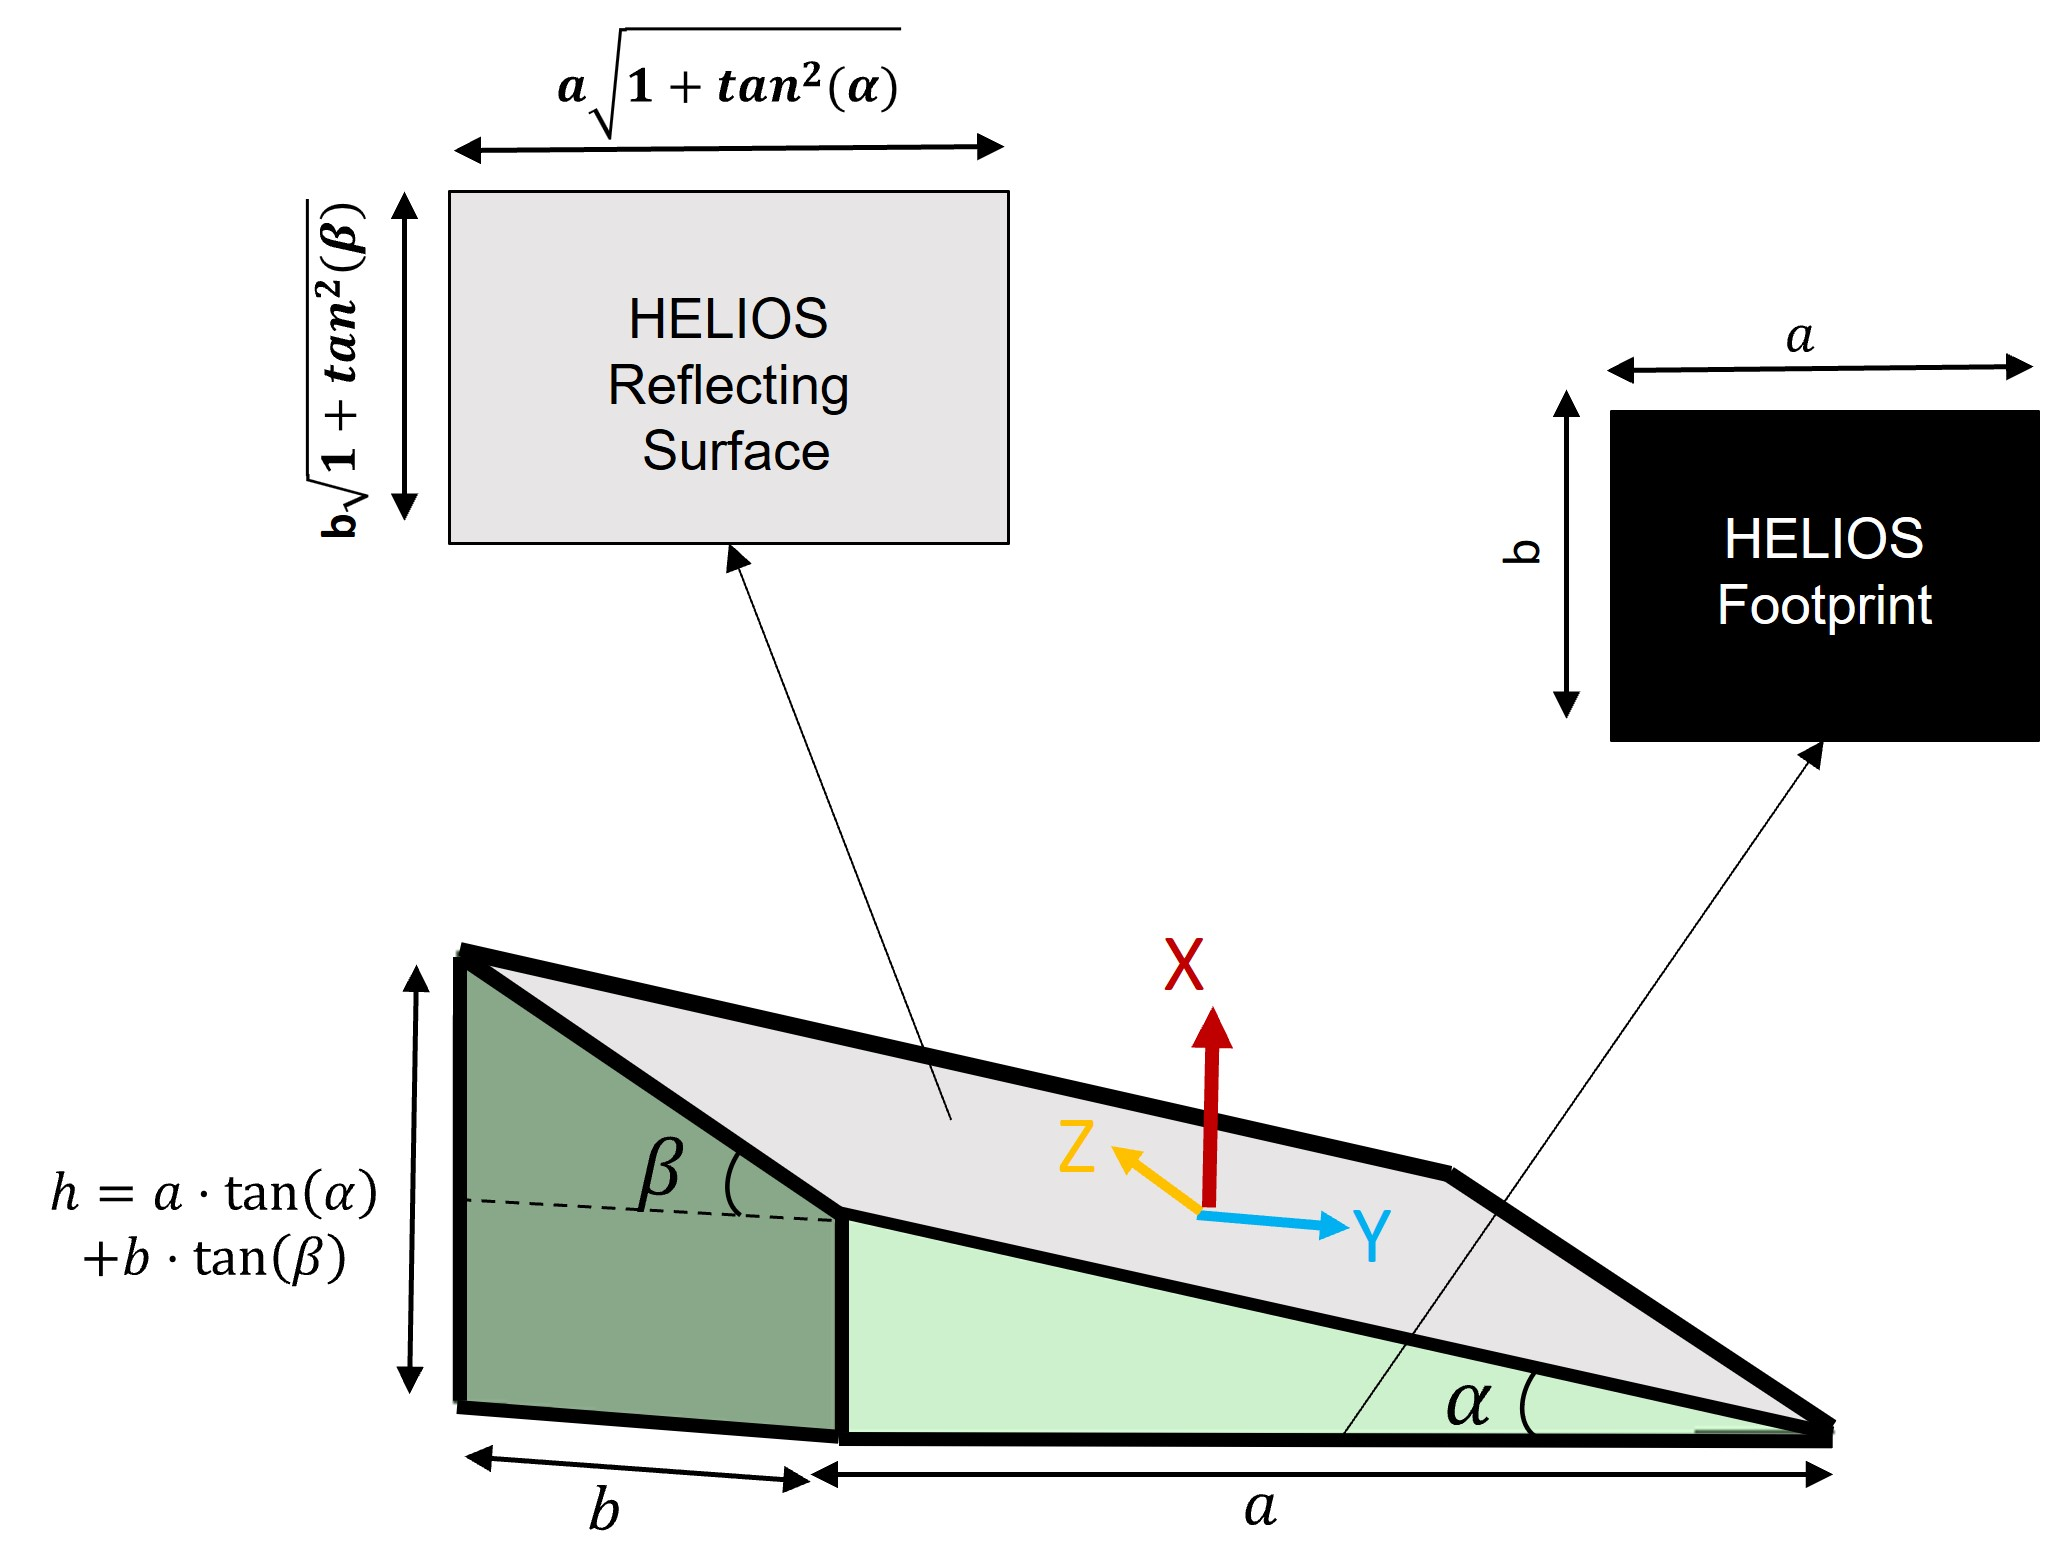
\includegraphics[width=0.5\linewidth]{images/Section 3 Images/HELIOS_footprint}
	\caption{Geometric relation between HELIOS footprint size given by ($a \cdot b$), and reflecting surface size given by ($a \cdot \sqrt{1+\tan^2(\alpha)} \cdot b \cdot \sqrt{1+\tan^2(\beta)}$), where $a$ and $b$ are the length and width of the module.}
	\label{fig:HELIOS_footprint}
\end{figure}
Furthermore, the slope angles $\alpha$, and $\beta$ of the HELIOS module affect the main lobe reflection angles $\theta_{Rx}$ and $\varphi_{Rx}$ as summarized by \Cref{HELIOS 2times beta} and \Cref{HELIOS 2times alpha}. As the Snell's law still holds along the shifted surface's normal vector, this rotation aspects is implemented by a coordinate transformation shifting by $\alpha$, and $\beta$. As a result, the angles of incidence $\theta_{Tx}$ and $\varphi_{Tx}$ in the equation are replaced by $\theta_{Tx}-\beta$ and $\varphi_{Tx}-\alpha$. The same holds for the angles of departure. To ensure that the beamwidth matches the simulated values, the literature already includes a scaling factor $\frac{1}{2}$ by default, allowing for a more precise match of the theoretical model with a HELIOS module's real-world behavior.

Based on all of the above changes, an individual HELIOS module exhibits the following bistatic RCS holding for $\theta_{Tx}$, $\varphi_{Tx}$, $\theta_{Rx}$, and $\varphi_{Rx} \in [-90, 90]^\circ$:

$	\sigma_{module}= 4 \cdot \pi \cdot \Gamma \cdot \left( \frac{\left( a \cdot \sqrt{1+\tan^2(\alpha)}\right) \cdot \left( b \cdot \sqrt{1+\tan^2(\beta)} \right) }{\lambda} \right) ^2 \left( \cos^2 \left( \theta_{Tx}-\beta \right) \cdot \cos^2 \left( \theta_{Rx}-\beta \right) \cdot \cos^2 \left( \varphi_{Rx}-\alpha \right) \right)$
\begin{equation} \label{Eq:HELIOS_module}
	\begin{aligned}
		& \left( \sinc \left( \frac{1}{2} \cdot k \cdot b \cdot \sqrt{1+\tan^2(\beta)} \cdot \left( \sin \left( \theta_{Rx}-\beta \right) \cdot \cos \left( \varphi_{Rx}-\alpha \right) -\sin \left( \theta_{Tx}-\beta \right) \cdot \cos \left( \varphi_{Tx}-\alpha \right) \right) \right) \right)^2\\
		&  \left( \sinc \left( \frac{1}{2} \cdot k \cdot a \cdot \sqrt{1+\tan^2(\alpha)} \cdot \left( \cos \left( \theta_{Rx}-\beta \right) \cdot \sin \left( \varphi_{Rx}-\alpha \right) -\cos \left( \theta_{Tx}-\beta \right) \cdot \sin \left( \varphi_{Tx}-\alpha \right) \right) \right) \right)^2 
	\end{aligned}
\end{equation}
Two $\sinc$ functions are presented in the equation, each of which individually affects the surface size's reflection properties for length and width. For the target's radar cross-section to be adequately represented, this separation is necessary. The diffraction phenomenon's $\sinc$ functions explain the reflecting surface's spatial extent along its dimensions, providing a thorough representation of the target's scattering characteristics. The equation provides a more accurate and complete model for radar analysis by accounting for the distinct impacts of width and length on the reflected signal.

The insertion of the adjustments mentioned in the \Cref{Table:Comparison flat plate and HELIOS} into the fundamental \Cref{RCS_flatplate} for a flat plate reflector leads to \Cref{Eq:HELIOS_module}, constituting our analytical model for the bistatic RCS of an individual HELIOS module.
\subsection{Assessment of Differences between Simulations and Analytical Model} \label{Assessment of Differences between Simulations and Analytical Model}
In this section, we will conduct a detailed comparison of EM simulations and our previously provided analytical model to check matching properties and, in particular, to determine the extent to which there are discrepancies.

\Cref{fig:absweep} shows the link between peak gain, defined as $\max\left(\sigma_{Module}\left(\varphi_{Rx}, \theta_{Rx}\right)\right)$, attained and reflector width $b$ in \si{\centi\meter}. The upper curves show the quadratic case in which $a=b$ in the range from \num{1} to \SI{100}{\centi\meter}, whereas the lower curves show the rectangular case in which $a$ is fixed to \SI{10}{\centi\meter} and $b$ again varies between \num{1} to \SI{100}{\centi\meter}. These curves are based on our study in \Cref{Simulative Analyses of HELIOS Reflector Modules} and related work in \Cref{coordinate systems}, show a steady increase in gain as the reflector size increases. Notably, one observes a strong match between simulations and our analytical model. Both the curves from the analytical model and EM simulation results meet when $a=b=\SI{10}{\centi\meter}$.
\begin{figure}[H]
	\centering
	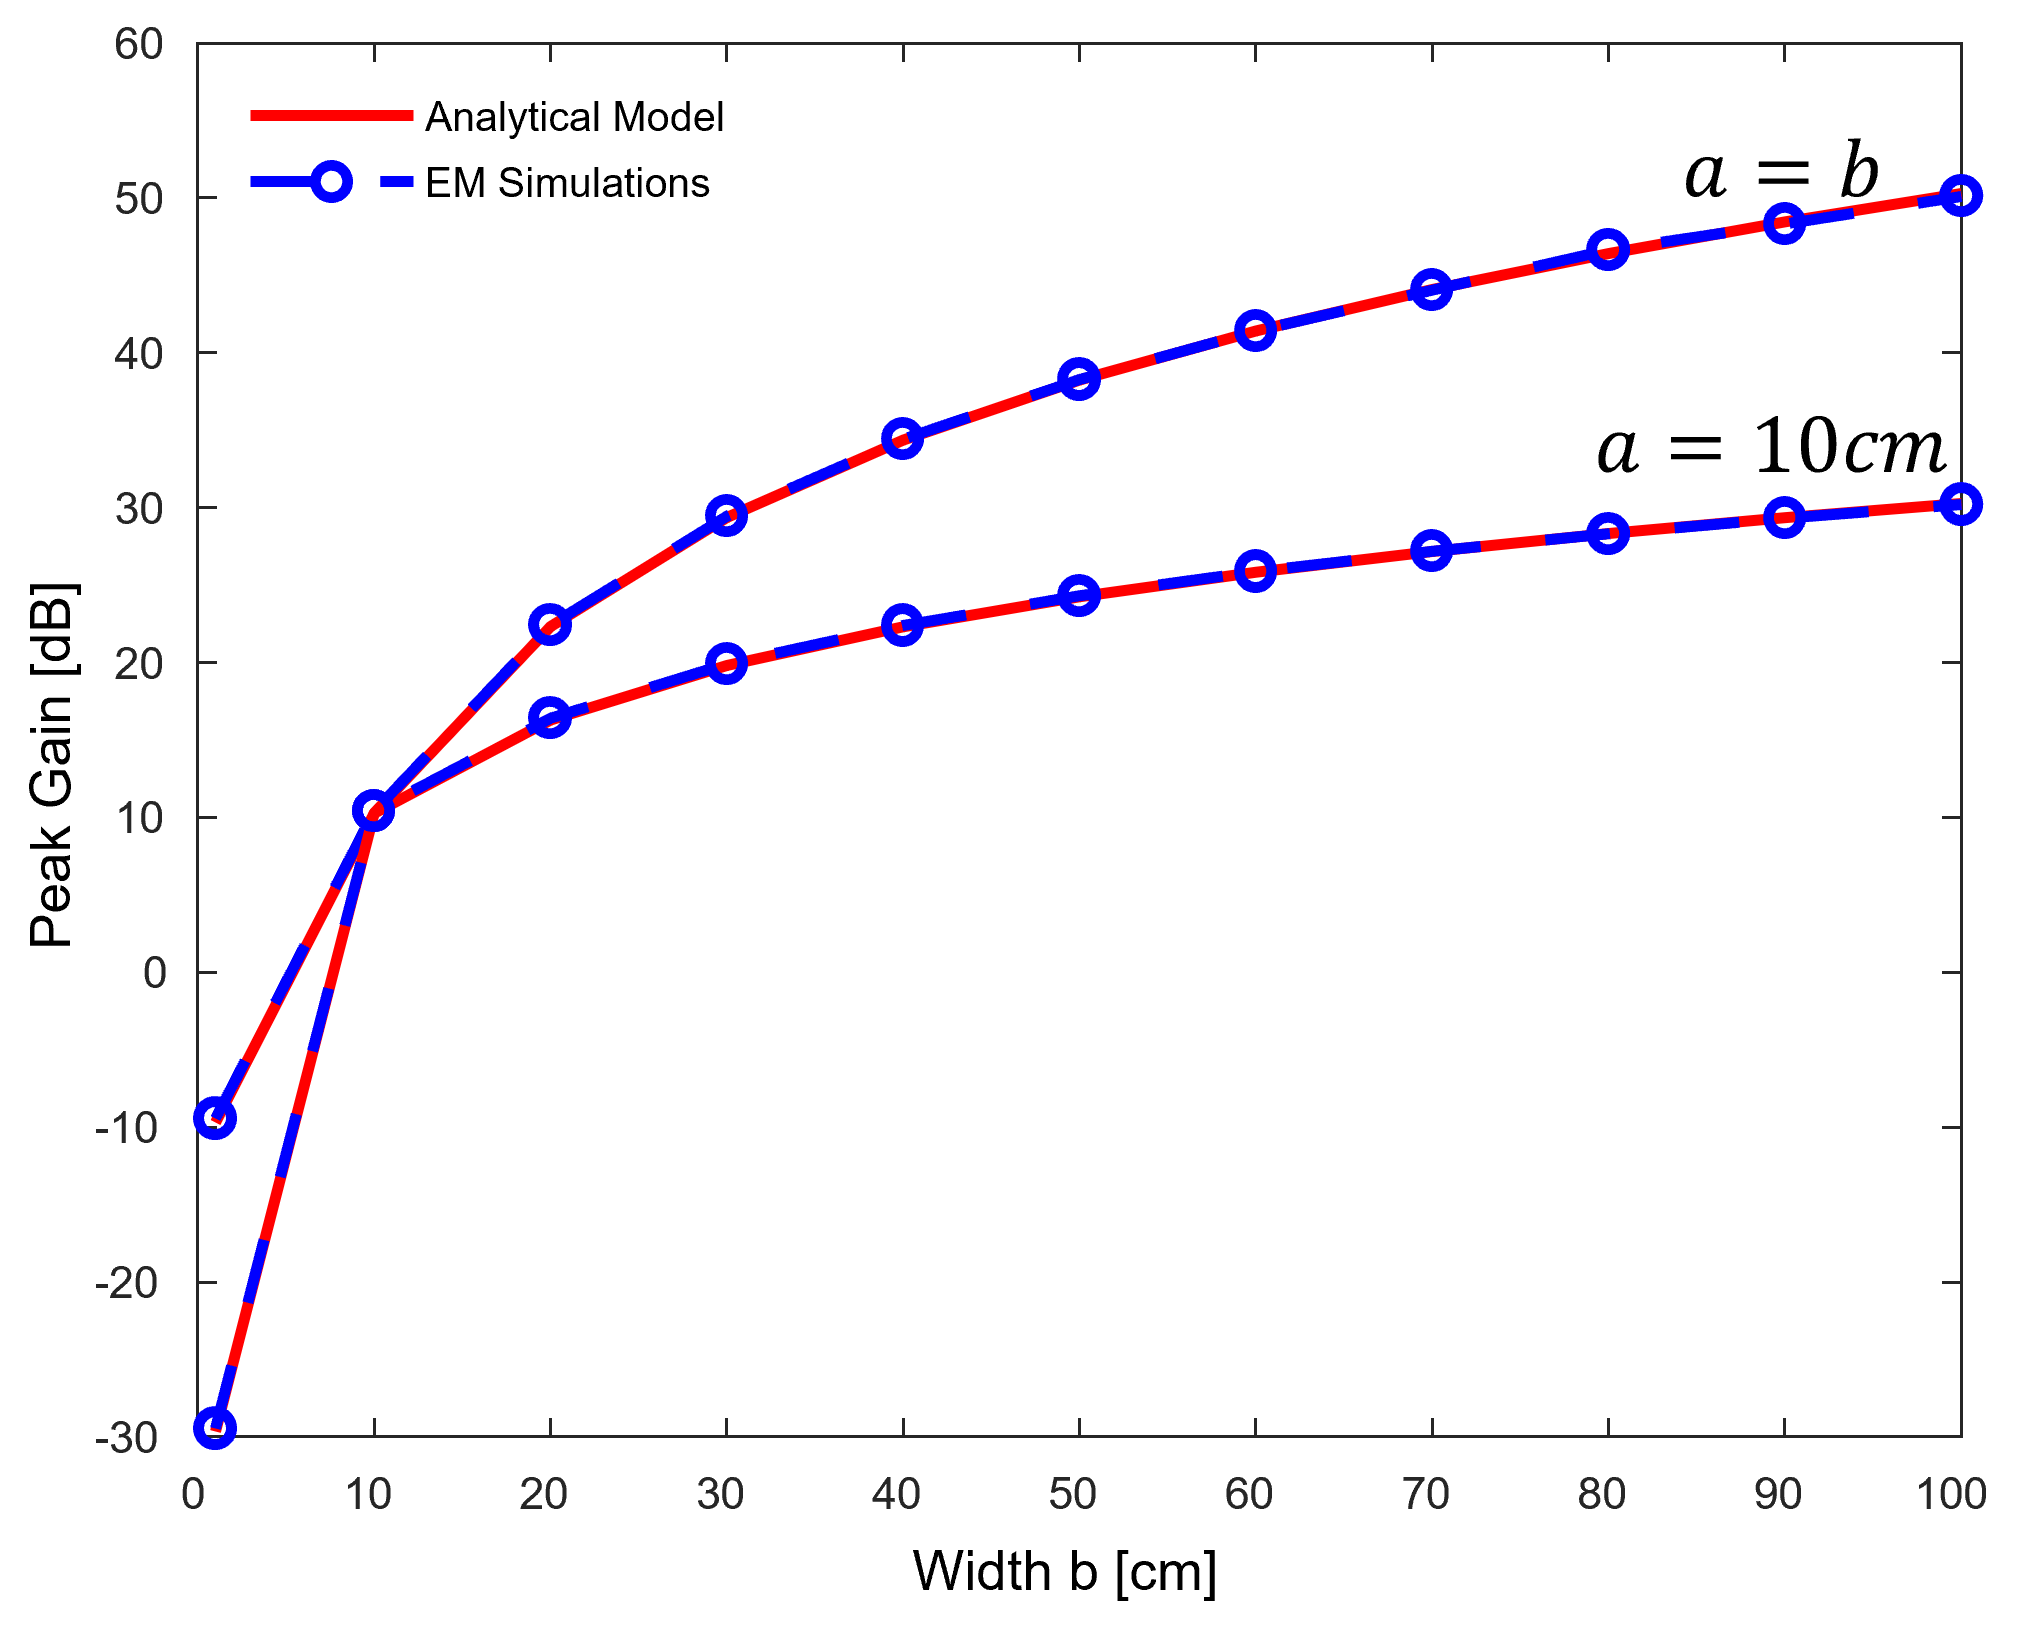
\includegraphics[width=0.7\linewidth]{images/Section 3 Images/a_b_sweep}
	\caption{Comparison of peak RCS value yielded by simulation and analytical model for rectangular $(\SI{10}{\centi\meter} \times b)$ and quadratic $(b \times b)$ HELIOS module footprints, where we observe a matching behavior. Further parameters: $\varphi_{Tx}=\theta_{Tx} = 0^\circ$ and, $\alpha_{m,n}=\beta_{m,n}=10^\circ$.}
	\label{fig:absweep}
\end{figure}

\Cref{fig:comparison1d} depicts the horizontal (left) and vertical (right) slices of the bistatic RCS patterns from both the simulations and analytical model, respectively, for HELIOS reflector modules configured with $a=\SI{10}{\centi\meter}$, $b=\SI{20}{\centi\meter}$, $\alpha=\num{10}^\circ$, and $\beta=\num{5}^\circ$, and given a \SI{28}{\giga\hertz} incident wave from direction $\varphi_{Tx}=\theta_{Tx}=\num{0}^\circ$.
\begin{figure}[tb]
	\centering
	\subfloat[Azimuth angle $\varphi_{Rx}$ variation for a HELIOS module when $\theta_{Rx}=0^\circ$ highlighting a match near the main lobe (green color) and a mismatch occurs further away (red color). ]{
		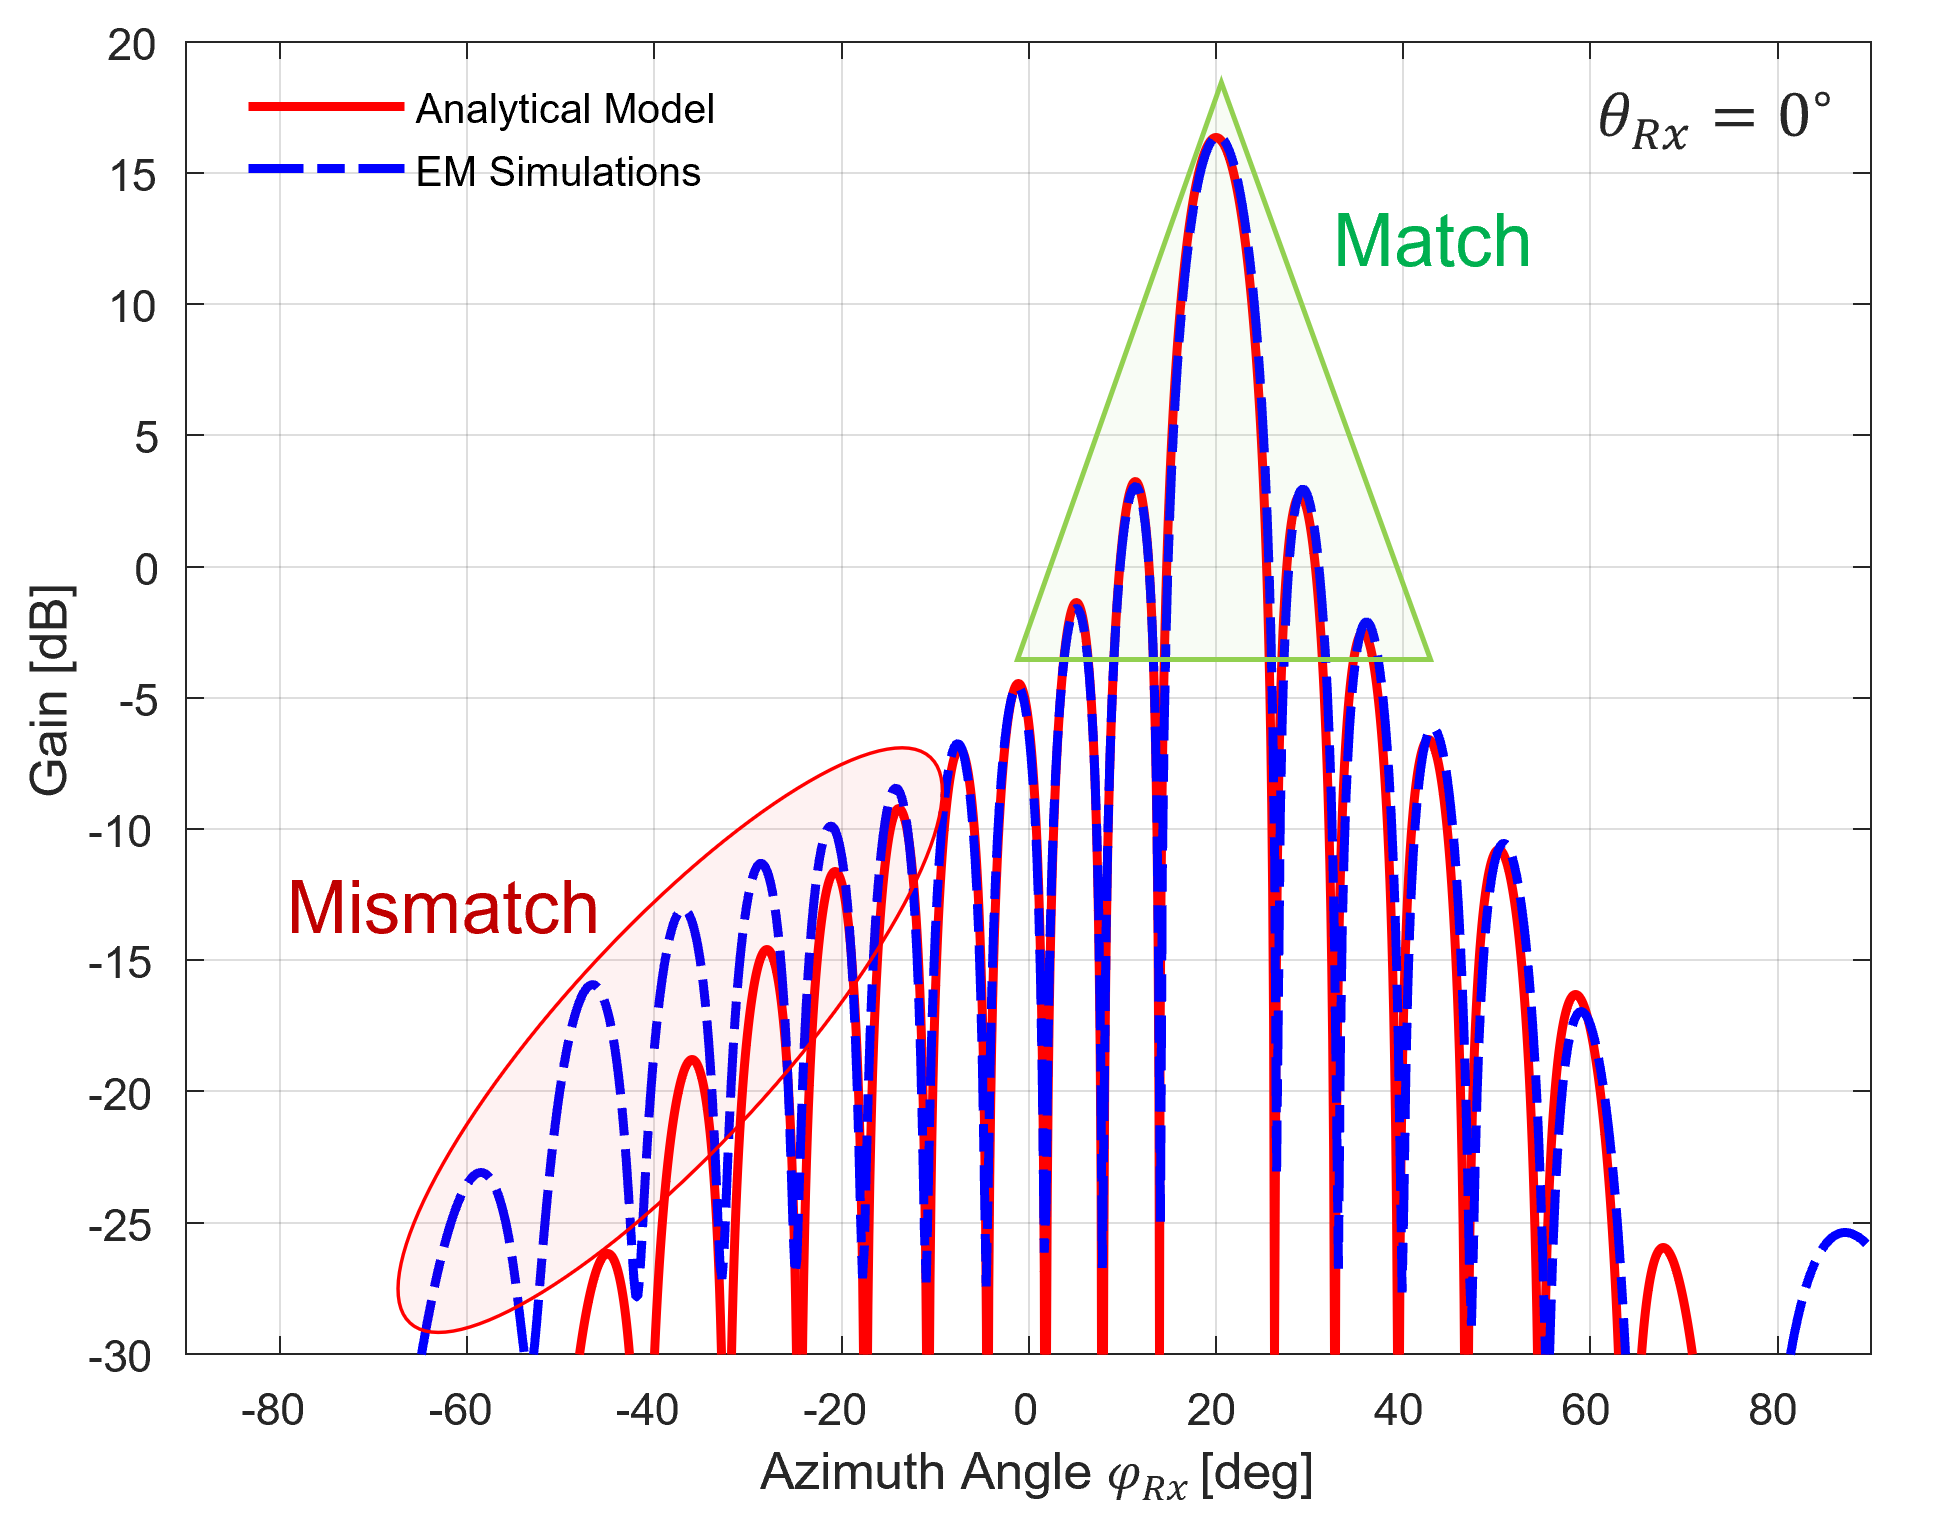
\includegraphics[width=0.46\linewidth]{images/Section 3 Images/comparison_1D_a}
		\label{fig:comparison1da}
	}
	\hfill
	\subfloat[Elevation angle $\theta_{Rx}$ variation for a HELIOS module when $\varphi_{Rx}=0^\circ$ highlighting a match (green color) overall.]{
		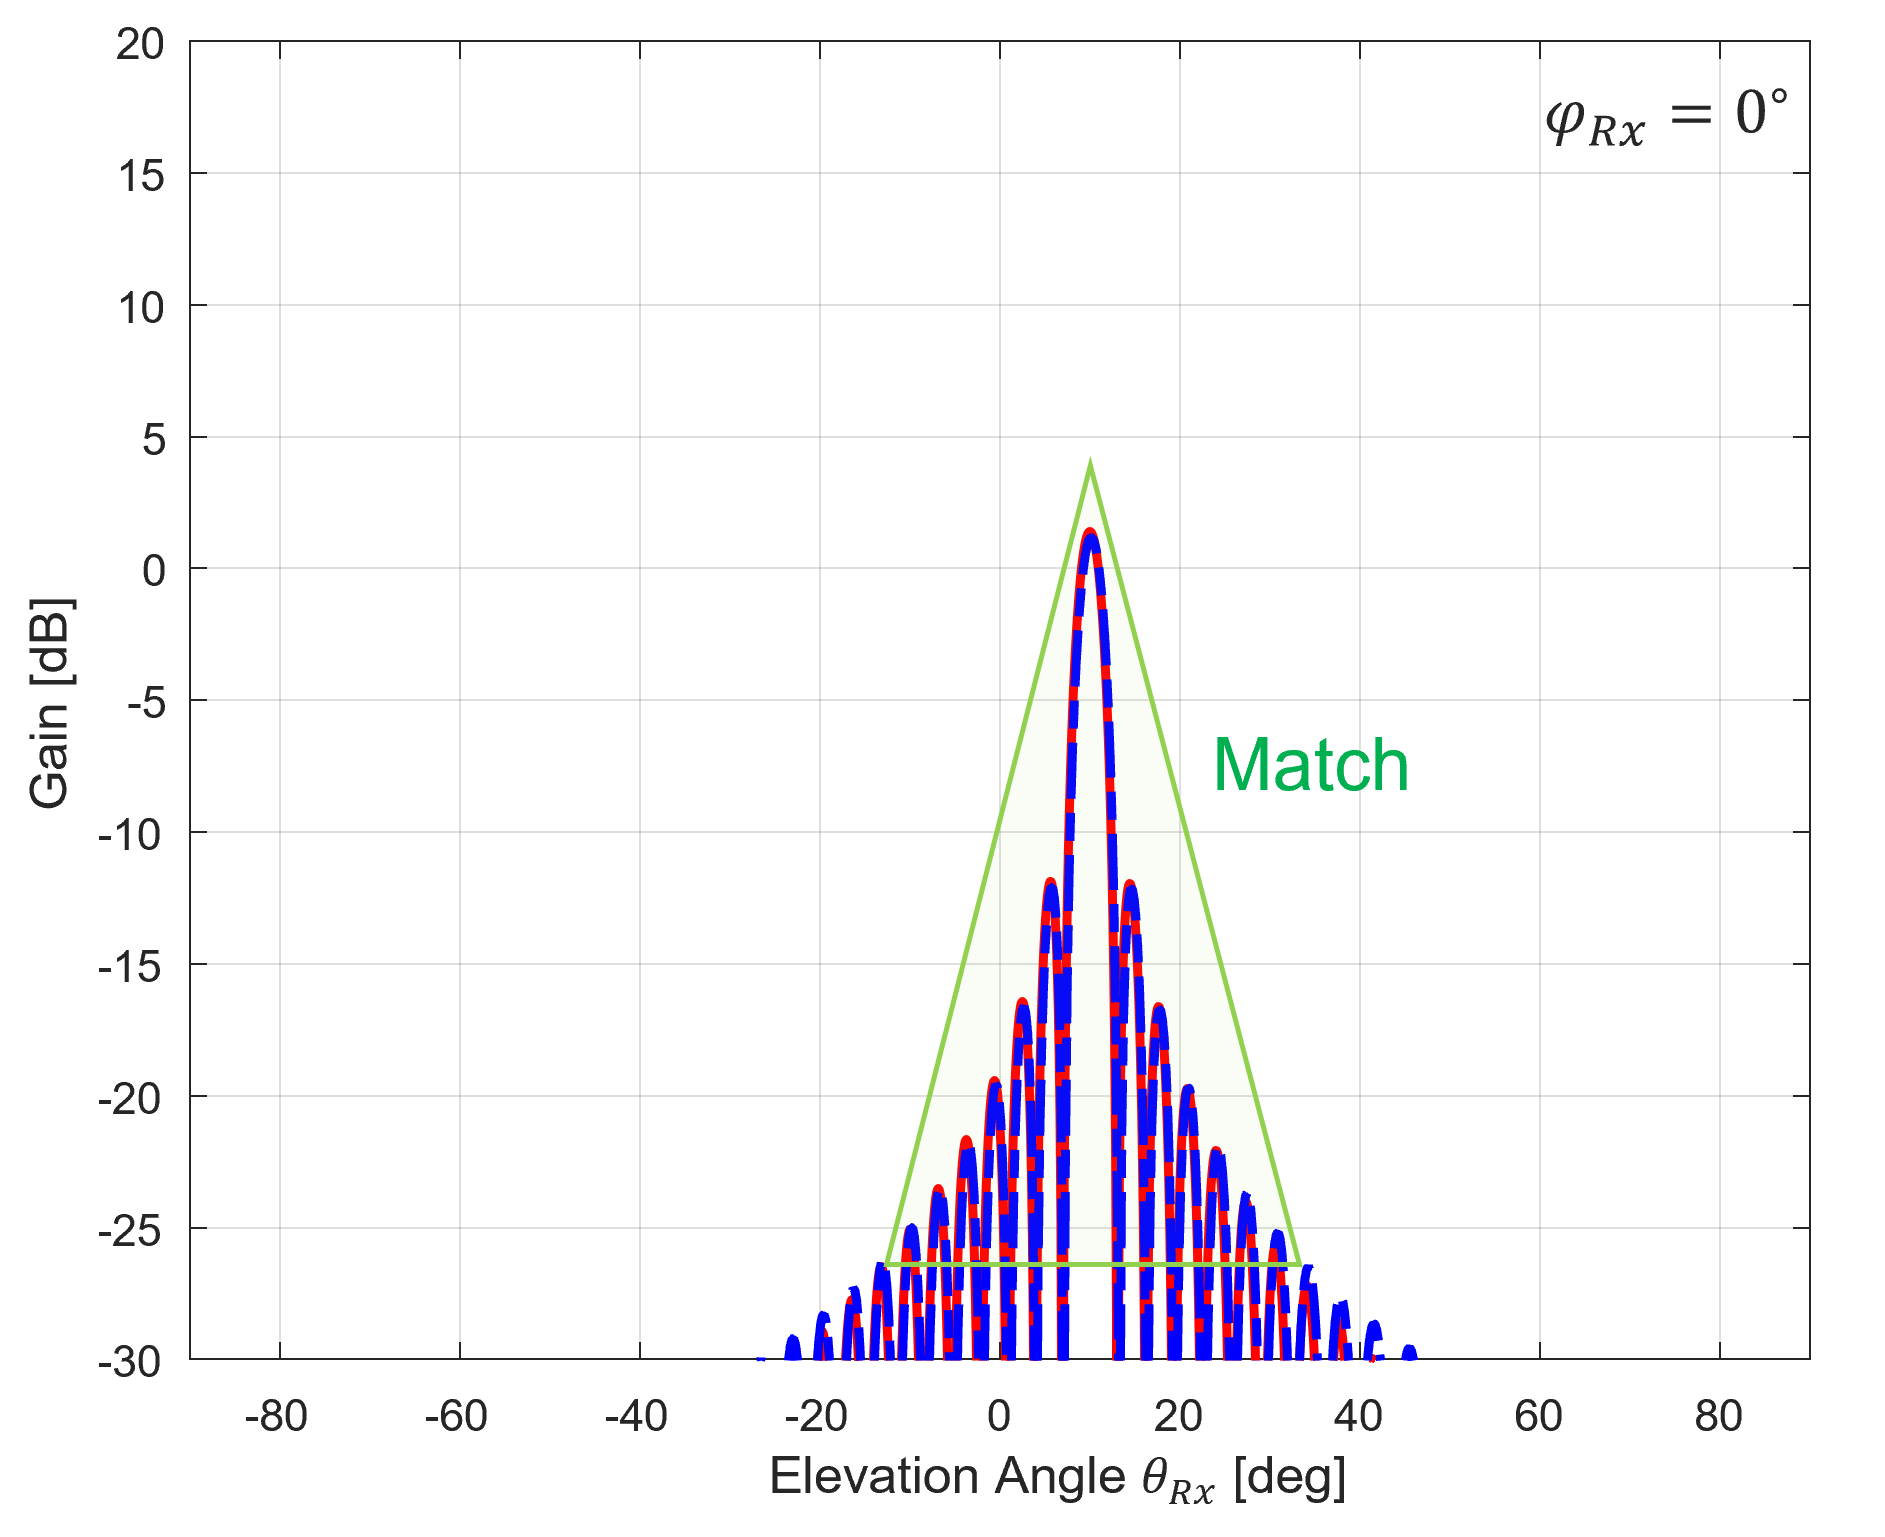
\includegraphics[width=0.45\linewidth]{images/Section 3 Images/comparison_1D_b}
		\label{fig:comparison1db}
	}
	\caption[Validating the HELIOS concept along azimuth and elevation angle at the receiver and highlighting the similarities and differences between simulated and analytical models for a HELIOS module when $a=\SI{10}{\centi\meter}$, $b=\SI{20}{\centi\meter}$, $\alpha=\num{10}^\circ$, and $\beta=\num{5}^\circ$, and both $\varphi_{Tx}=\theta_{Tx}=\num{0}^\circ$. A notable match in the peak gain is observed between the simulation results and the analytical model.]{Validating the HELIOS concept along azimuth and elevation angle at the receiver and highlighting the similarities and differences between simulated and analytical models for a HELIOS module when $a=\SI{10}{\centi\meter}$, $b=\SI{20}{\centi\meter}$, $\alpha=\num{10}^\circ$, and $\beta=\num{5}^\circ$, and both $\varphi_{Tx}=\theta_{Tx}=\num{0}^\circ$. A notable match in the peak gain is observed between the simulation results and the analytical model.}
	\label{fig:comparison1d}
\end{figure}
In the horizontal pattern slice on \Cref{fig:comparison1da}, we observe the RCS peaks at $\varphi_{Rx} = 20^\circ = -\varphi_{Tx} + 2\cdot\alpha$, thus confirming \Cref{HELIOS 2times alpha}. Similarly, the vertical RCS pattern slices in \Cref{fig:comparison1db} confirm that the RCS peaks of simulation and analytical model are indeed at $\theta_{Rx} = 10^\circ = -\theta_{Tx} + 2\cdot\beta$, cf. \Cref{HELIOS 2times beta}. The beamwidth along $\varphi_{Rx}$ depends on reflector dimension $a$, whereas $\theta_{Rx}$ depends on $b$. In \Cref{fig:comparison1d}, as the dimensions $b >a$, the vertical beamwidth (right) is narrower than the horizontal (left).

The interesting part in both these figures is that the simulated values closely match the analytical values, displaying exceptional behavior in the properties of their main and the first-order, $N$-th-order side lobes. But farther from the main lobes we see the mismatch along the azimuth angle, as depicted in \Cref{fig:comparison1da} (red-colored). Our main region of interest shows a lot of similarities to that of simulated results (green-colored). Furthermore, a closer examination of these figures reveals the importance of beamwidth in the behavior of these systems which depends on the size of the reflector.

\Cref{fig:heatmap1d} shows the bistatic RCS heatmaps along reflection angles $\varphi_{Rx}$ and $\theta_{Rx}$ with the gain being color coded. This allows for a qualitative visual comparison of the behavior attained by simulations and via the analytical model. The following parameters are used by the figure below: $a=b=\SI{10}{\centi\meter}$ and $\alpha=\beta=\num{10}^\circ$ with $\varphi_{Tx}=\theta_{Tx}=\num{0}^\circ$. Notably, the reflected angle at which the maximum peak is attained validates the HELIOS concept. A closer look at the RCS heatmap behavior in the figure shows that the main lobe and the side lobes in both the analytical model and EM simulations match.

\begin{figure}[tb]
	\centering
	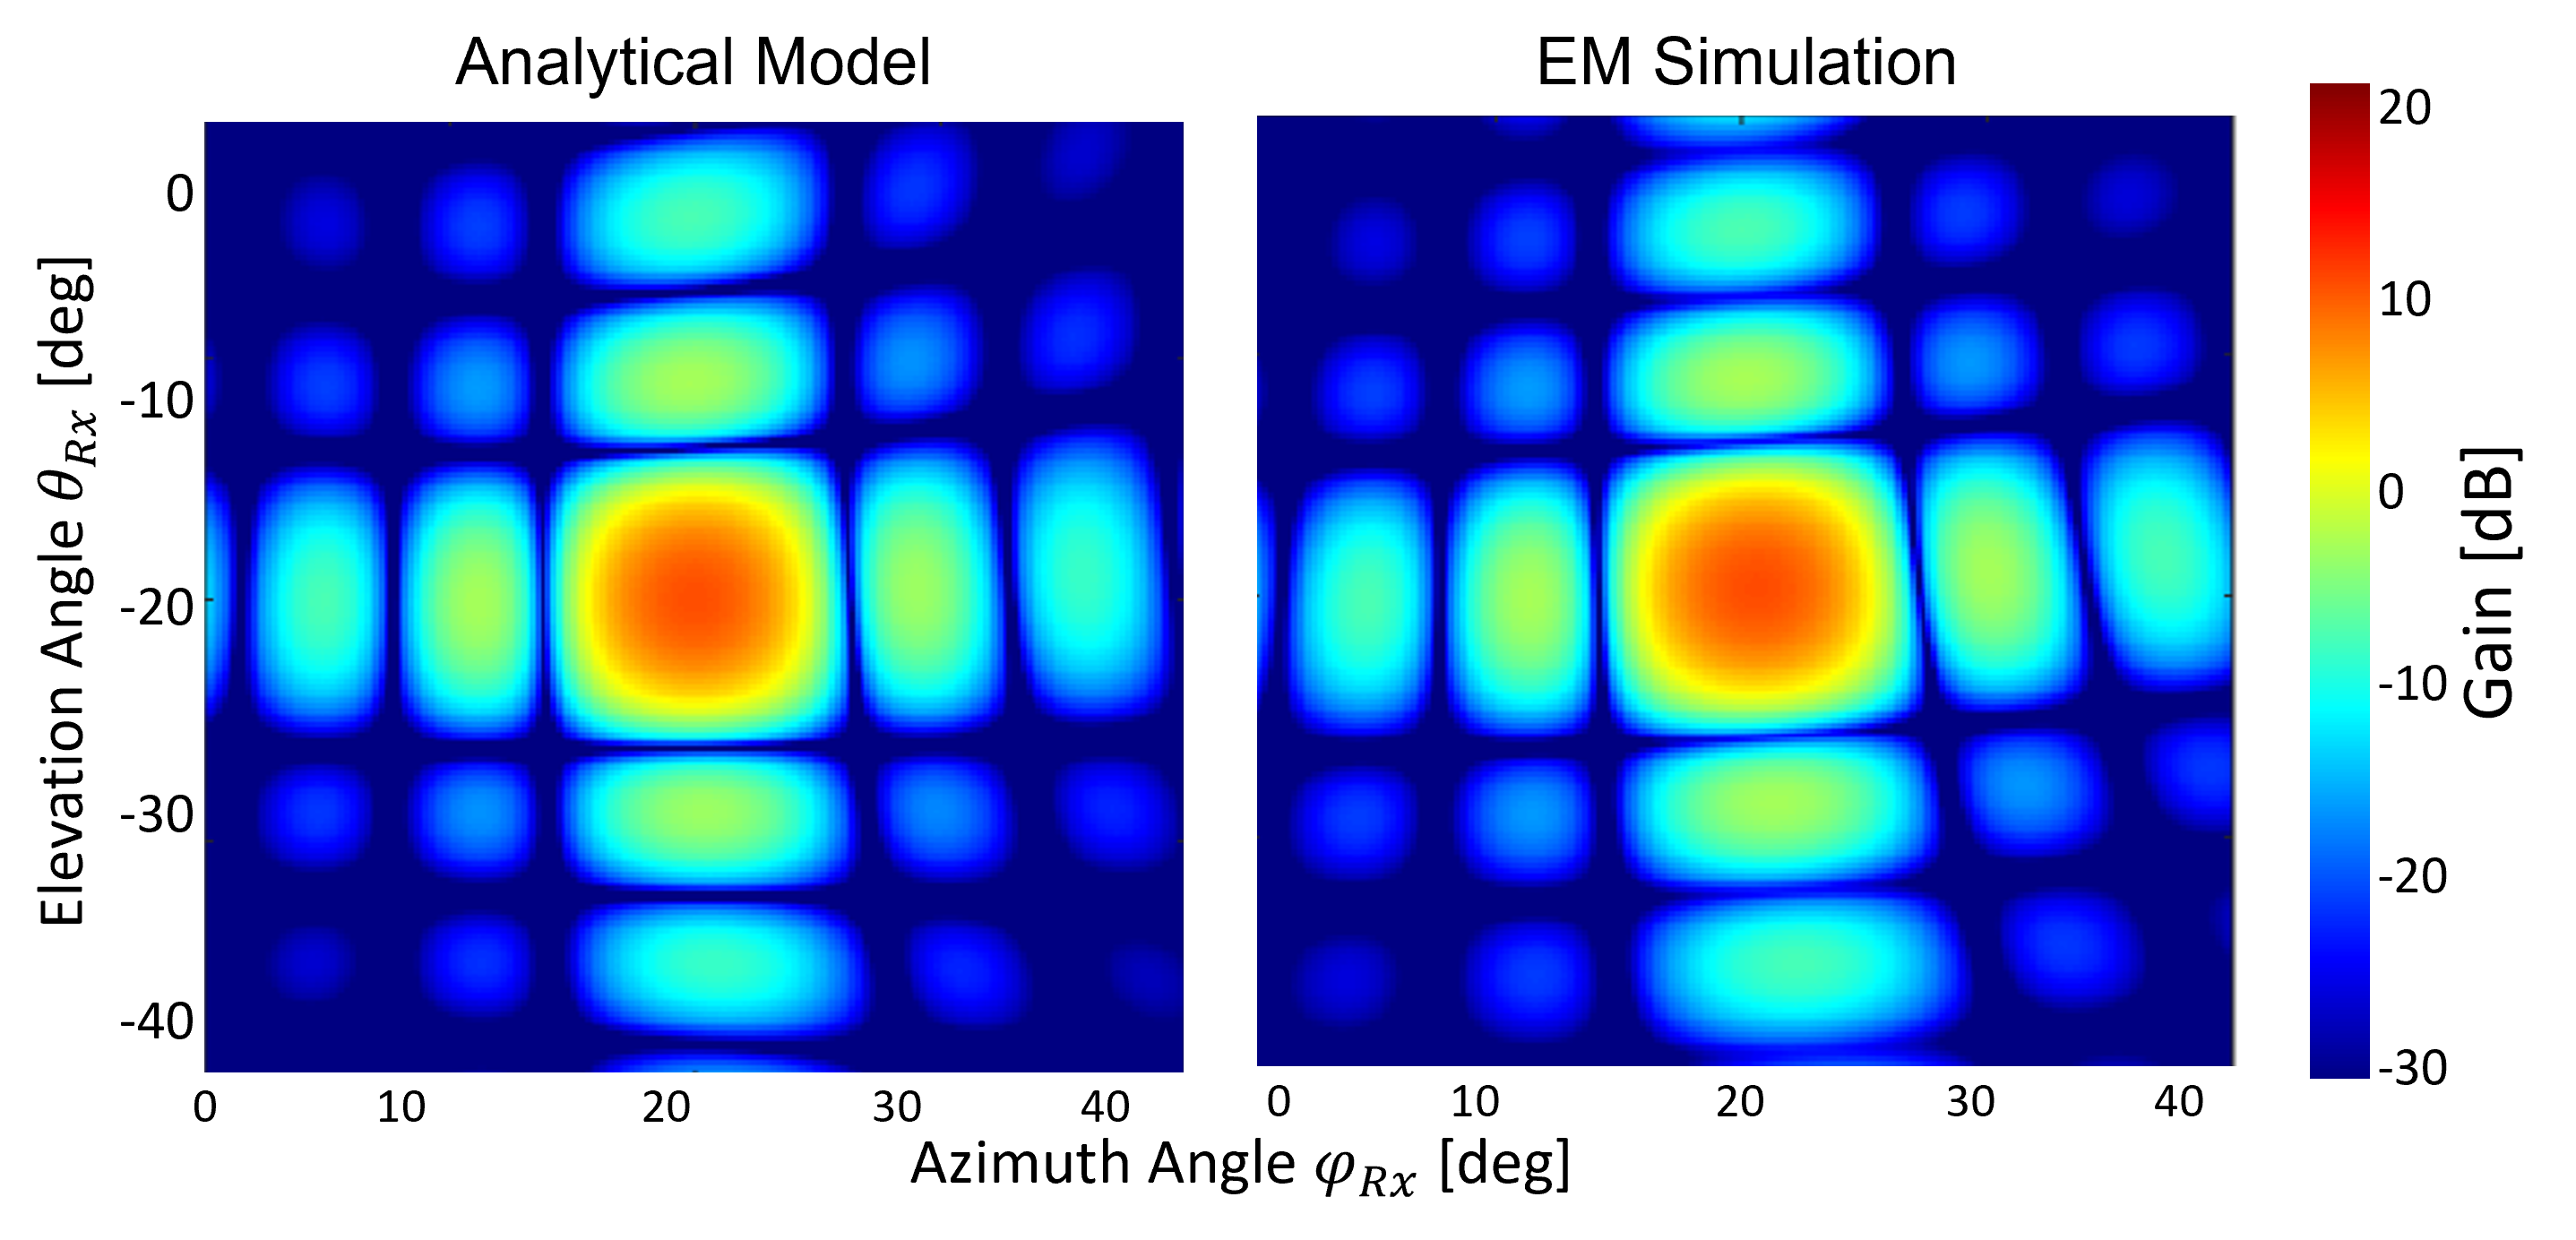
\includegraphics[width=0.82\linewidth]{images/Section 3 Images/Heatmap_1D}
	\caption{Sample RCS pattern of individual HELIOS module ($1 \times 1$): (left) analytical model, (right) EM simulations for parameters $a=b=\SI{10}{\centi\meter}$ and $\alpha=\beta=\num{10}^\circ$ at \SI{28}{\giga\hertz} frequency with peak gain of \SI{10.4}{\decibel}.}
	\label{fig:heatmap1d}
\end{figure}
Further adaptation of the HELIOS reflector module at \SI{38}{\giga\hertz} frequency is seen in \Cref{fig:heatmap_38GHz}. The peak gain by the analytical model and EM simulation results at \SI{28}{\giga\hertz} frequency is around \SI{10.4}{\decibel}, whereas at \SI{38}{\giga\hertz} frequency is \SI{13.0}{\decibel}. Because of their shorter wavelengths, reflectors typically show better gain characteristics at higher frequencies, such as \SI{38}{\giga\hertz}, allowing for more directed and focused signal propagation. This variant highlights how carrier frequencies and reflector performance interact intricately in 5G mmWave scenarios, impacting the network's overall signal propagation and coverage properties.
\begin{figure}[H]
	\centering
	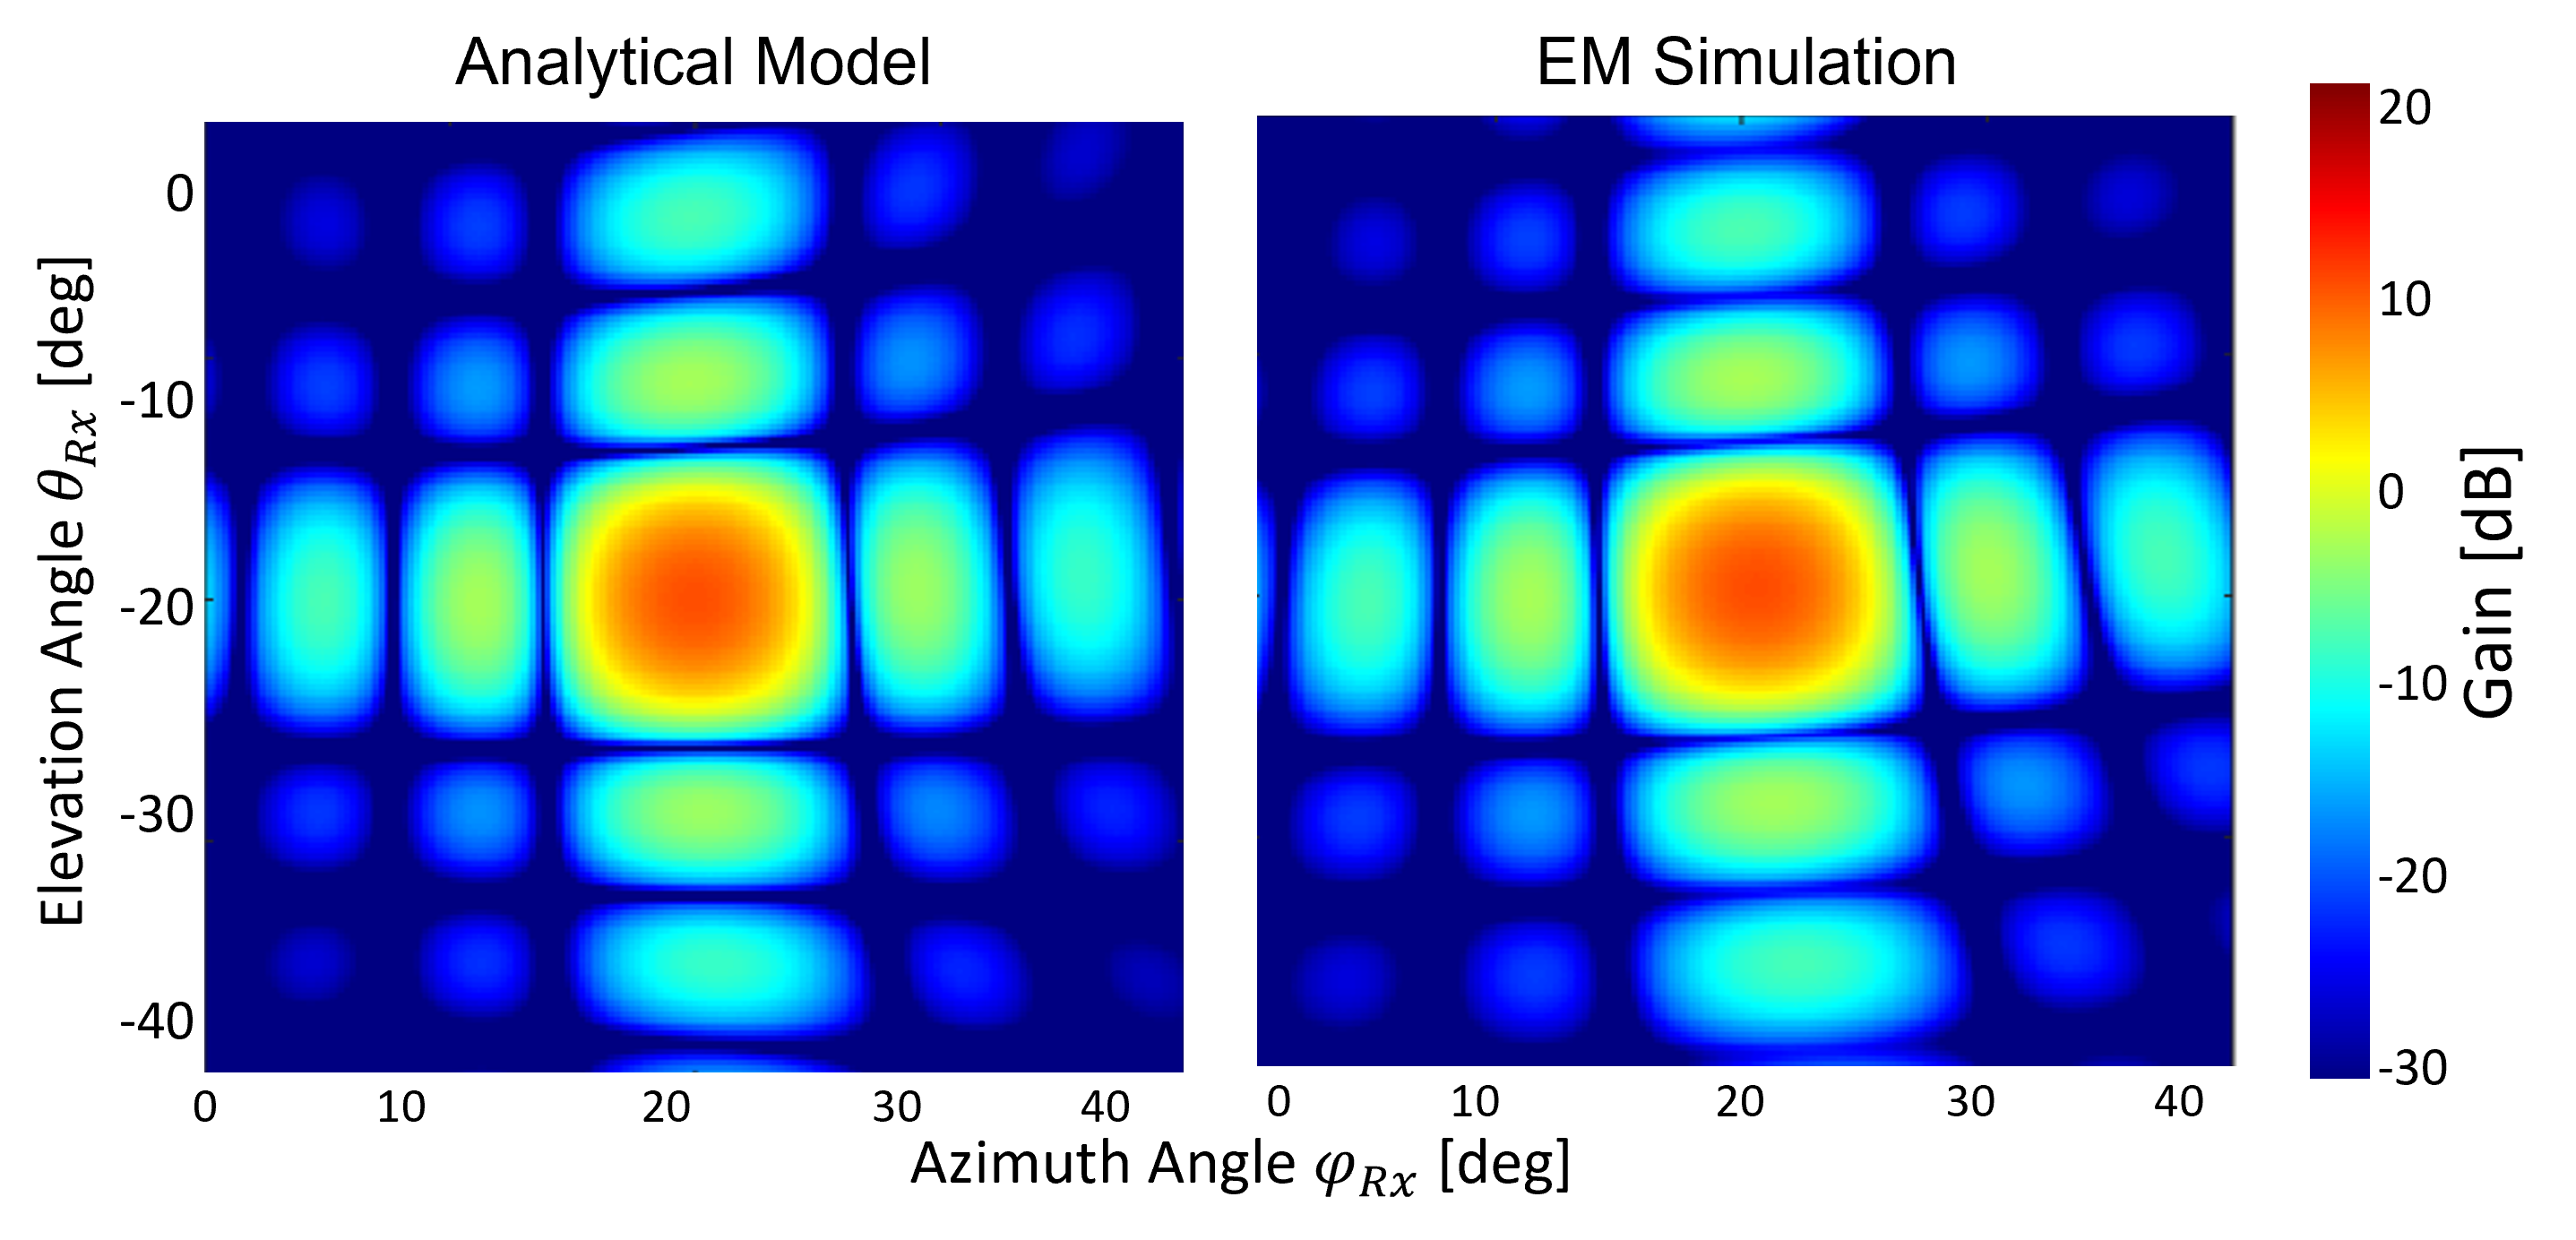
\includegraphics[width=0.82\linewidth]{images/Section 3 Images/Heatmap_1D}
	\caption{Sample RCS pattern of individual HELIOS module ($1 \times 1$): (left) analytical model, (right) EM simulations for parameters $a=b=\SI{10}{\centi\meter}$ and $\alpha=\beta=\num{10}^\circ$ at \SI{38}{\giga\hertz} frequency with peak gain of \SI{13.0}{\decibel}.}
	\label{fig:heatmap_38GHz}
\end{figure}
\section{Analytical Model for Multi-Module HELIOS Reflectors} \label{Simulation and Modeling of HELIOS Reflectors}
In this section, we now focus on HELIOS reflectors in the form of an array of HELIOS modules. Owing to this, our model from \Cref{Analytical Modeling of HELIOS Modules} is extended and subsequently reevaluated. An initial extension is carried out in \Cref{Independent Composition of Overall Reflection Characteristics}, after which the accuracy model is thoroughly assessed by looking at three case studies. The discussion of self-shadowing issues that could surface between certain selected modules of a reflector's modules is then covered in \Cref{Improved Model using Inter-module Relations}, depending on how it is configured. This concentrated examination seeks to improve the accuracy of the analytical model that is introduced in this thesis, guaranteeing a thorough comprehension and improvement of its functions.
\subsection{Independent Superposition of Overall Reflection Characteristics} \label{Independent Composition of Overall Reflection Characteristics}
The independent composition of overall reflection properties entails combining many separate HELIOS modules to realize fully-fledged reflectors or arbitrary characteristics. Thus, depending on a single, monolithic reflector, which has limitations, this modular approach provides a great degree of flexibility and adaptability. The established formula shown in \Cref{Eq:RCS_SUMMATION} allows for the superposition of the individual RCS patterns of the HELIOS module, thereby providing a formula for the overall HELIOS reflector array. Whereas one could use the bistatic RCS pattern from \Cref{Analytical Modeling of HELIOS Modules}, cf. \Cref{Eq:HELIOS_module}, we propose a minor variation in the form of factors $M/2$ and $N/2$ (inside the $\sinc$ function) considering the overall number of modules along $y$- and $z$-axes, see \Cref{Eq:HELIOS_array}.

The below equations describe the HELIOS reflector array as a whole, and it provides a baseline for comparing different configured models' RCS behavior. Notably, the beamwidth factor is influenced by the factors $M/2$ and $N/2$ in the equation. This parameter was successfully applied to a single HELIOS module with factors of $1/2$ each, see \Cref{Eq:HELIOS_module}.
\begin{equation}\label{Eq:RCS_SUMMATION}
	\sigma_{Array}= \left(\sum_{n=1}^{N}\sum_{m=1}^{M} \sqrt{\sigma_{module} \left( a_{m,n}, b_{m,n}, \alpha_{m,n}, \beta_{m,n} \right) } \right)^2,
\end{equation}
with
\begin{equation} \label{Eq:HELIOS_array}
	\footnotesize
	\begin{aligned}
		 \sigma_{module} &=4 \cdot \pi \cdot \Gamma \cdot \left( \frac{\left( a_{m,n}\sqrt{1+\tan^2(\alpha_{m,n})}\right) \cdot \left( b_{m,n} \sqrt{1+\tan^2(\beta_{m,n})} \right) }{\lambda} \right) ^2\\
		&\left( \cos^2 \left( \theta_{Tx}-\beta_{m,n} \right) \cdot \cos^2 \left( \theta_{Rx}-\beta_{m,n} \right) \cdot \cos^2 \left( \varphi_{Rx}-\alpha_{m,n} \right) \right)\\
		& \left( \sinc \left( \frac{M}{2} \cdot k \cdot b_{m,n} \sqrt{1+\tan^2(\beta_{m,n})} \cdot \left( \sin \left( \theta_{Rx}-\beta_{m,n} \right) \cdot \cos \left( \varphi_{Rx}-\alpha_{m,n} \right) -\sin \left( \theta_{Tx}-\beta_{m,n} \right) \cdot \cos \left( \varphi_{Tx}-\alpha_{m,n} \right) \right) \right) \right)^2\\
		&  \left( \sinc \left( \frac{N}{2} \cdot k \cdot a_{m,n} \sqrt{1+\tan^2(\alpha_{m,n})} \cdot \left( \cos \left( \theta_{Rx}-\beta_{m,n} \right) \cdot \sin \left( \varphi_{Rx}-\alpha_{m,n} \right) -\cos \left( \theta_{Tx}-\beta_{m,n} \right) \cdot \sin \left( \varphi_{Tx}-\alpha_{m,n} \right) \right) \right) \right)^2 
	\end{aligned}
\end{equation}

Three in-depth case studies are conducted to validate this equation. In the first investigation, RCS patterns from various setups are compared. An ECDF comparison between the analytical model and EM simulation results of the HELIOS reflector array is carried out in the second study. The third study provides a comprehensive analysis of the equation's performance in various settings by examining various configurations and sensible beamwidth factors. Together, these case studies advance our understanding of the RCS behavior and the versatility of the equation in various reflector array configurations.
\subsubsection{Case Study 1: RCS Pattern Comparison for Different HELIOS Configurations}
For validation of \Cref{Eq:HELIOS_array}, we study the peak RCS gains of different dimensions of HELIOS arrays in \Cref{fig:arraymax}. In particular, we examined arrays with dimensions of $\num{1}\times N$ and $M\times N$, where $M$ and $N$ are integers between \num{1} and \num{8}. Whereas, there is already a noteworthy degree of consistency, there are nonetheless differences against the simulation results. For example, for the $\num{1}\times \num{8}$ array depicted on the left side, there is a difference of about \SI{0.4}{\decibel} between the EM simulation results and our analytical model. If we consider the $\num{8}\times \num{8}$ array on the right side, the difference increases to a more noticeable \SI{1.2}{\decibel}. As we show in \Cref{Improved Model using Inter-module Relations}, this is due to self-shadowing between the individual HELIOS modules.

A thorough bistatic RCS heatmap comparison for $\num{2}\times \num{2}$, $\num{4}\times \num{4}$, and $\num{8}\times \num{8}$ HELIOS reflectors arrays is carried out to analyze the various analytical and simulation findings, where we observe a match in the behavior, as shown in \Cref{fig:heatmaparraz}. Interestingly, a pattern emerges from the observations: both the simulative and analytical model beams show a notable narrowing effect with increasing gains as the reflector footprint grows.
\begin{figure}[H]
	\centering
	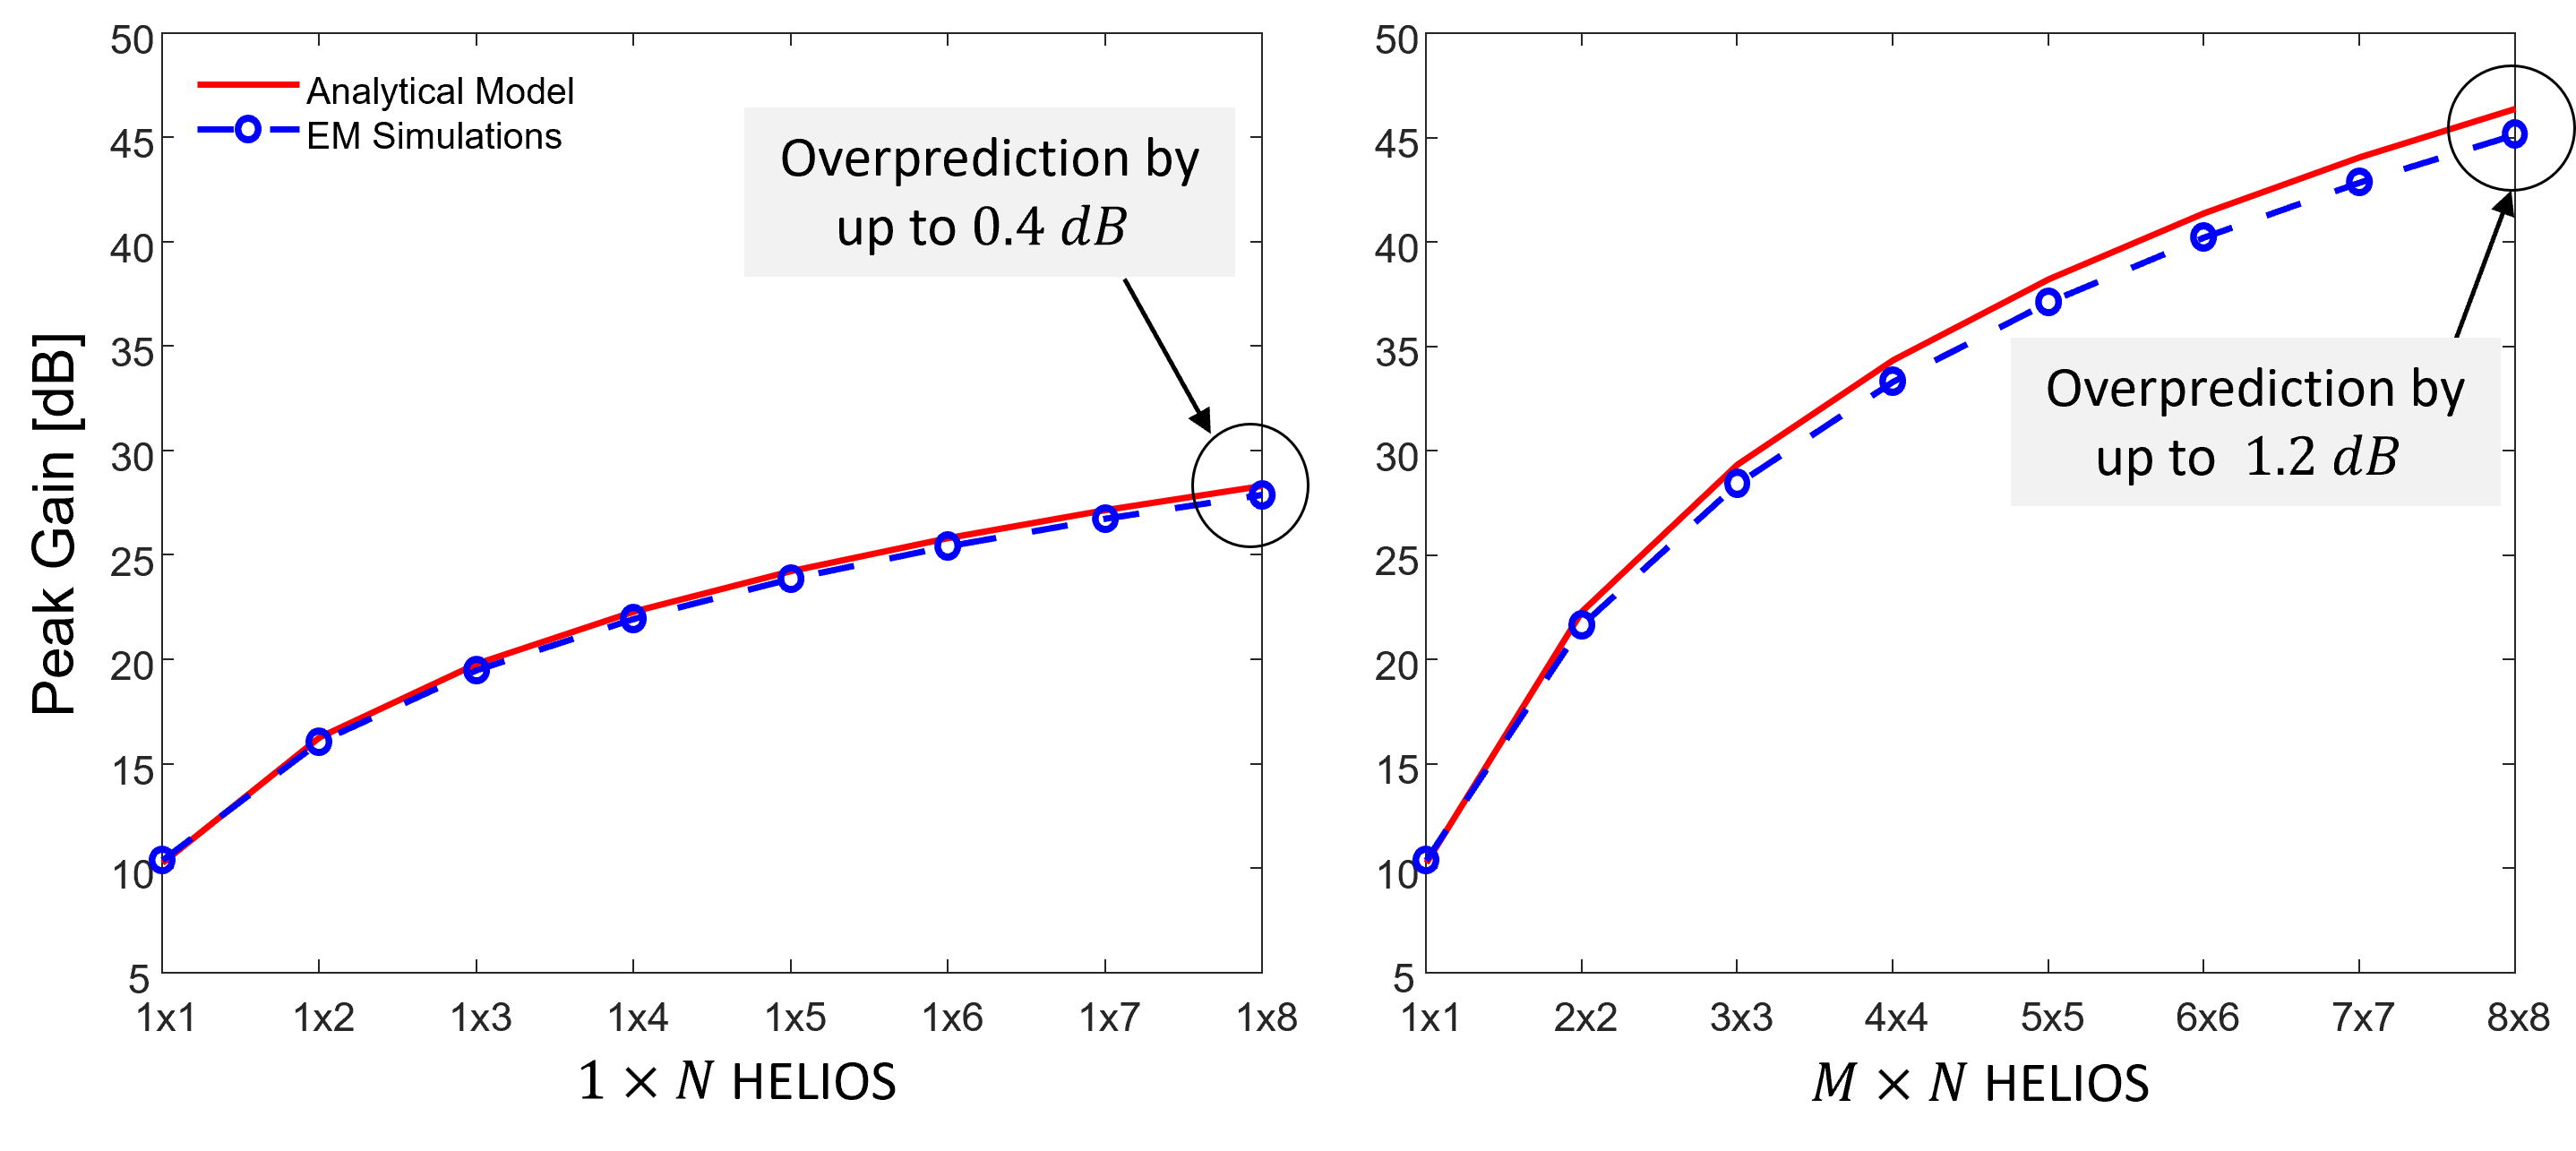
\includegraphics[width=1.0\linewidth]{images/Section 3 Images/Array_max}
	\caption{Plot against HELIOS array and maximum gain between simulated and analytical model highlighting the difference in gain in $\si{\decibel}$ for the case when $\alpha_{m,n}=\beta_{m,n}=10^\circ$ and $a_{m,n}=b_{m,n}= \SI{10}{\centi\meter}$ for $M=N\in[1:8]$ at \SI{28}{\giga\hertz} frequency.}
	\label{fig:arraymax}
\end{figure}
\begin{figure}[tb]
	\centering
	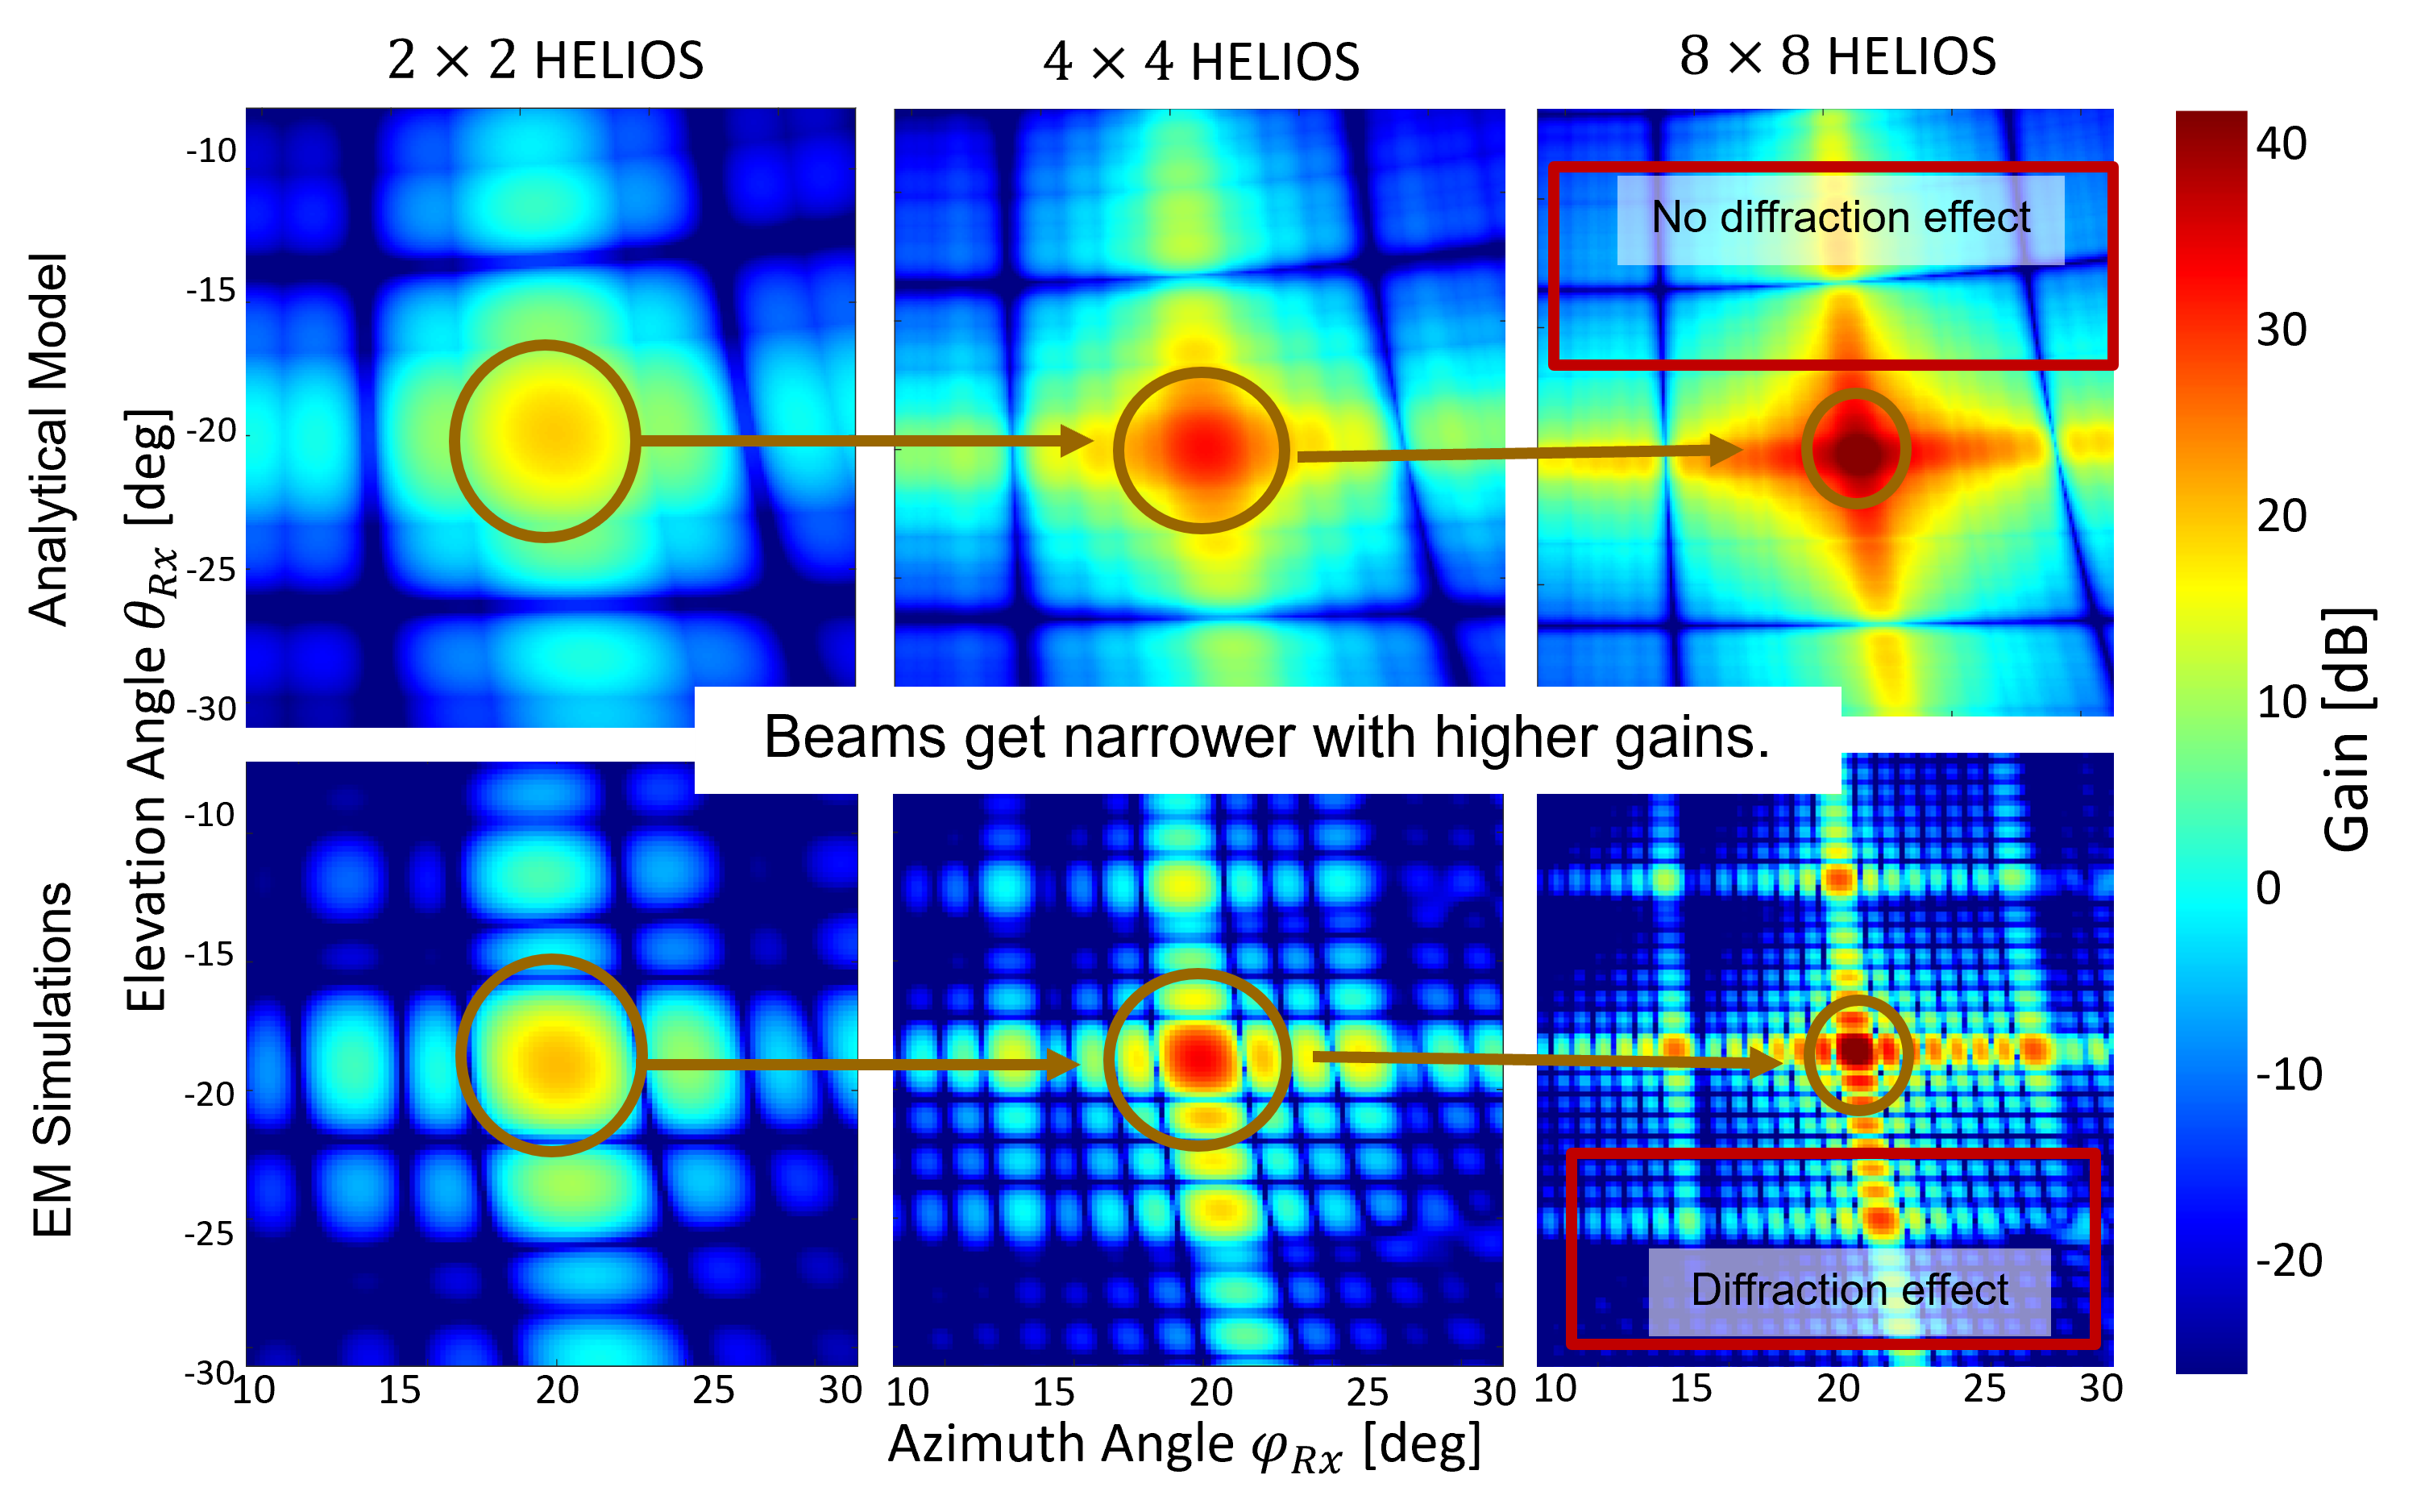
\includegraphics[width=1.0\linewidth]{images/Section 3 Images/Heatmap_arraz}
	\caption{RCS pattern behavior of HELIOS reflectors with different number of modules for simulation and analytical model highlighting the similarities in gains and beam patterns without the consideration of diffraction effect for $\alpha_{m,n}=\beta_{m,n}=10^\circ$ and $a_{m,n}=b_{m,n}= \SI{10}{\centi\meter}$. }
	\label{fig:heatmaparraz}
\end{figure}
Extending our analysis beyond the main lobe, we observe a limitation of our analytical model: diffraction effects are not included in the analytical model by default, as we are so far considering the models independently. This aspect can be addressed by future work. In the later part of this section, we refer to \Cref{Improved Model using Inter-module Relations} illustrates a similar fine-tuning of our model by considering inter-module shadowing effects.
\subsubsection{Case Study 2: ECDF Comparison of Analytical Model and EM Simulation Results for HELIOS Reflector Array.}
With an emphasis on both $\num{2}\times \num{2}$ and $\num{8}\times \num{8}$ HELIOS array configurations with $a_{m,n}=b_{m,n}=\SI{10}{\centi\meter}$, \Cref{fig:ECDF_HELIOS_array} depicts the ECDFs along the realized RCS gains which focuses on the performance differences between analytical and simulated values. As annotated in the plot, the more to the right the overall distribution curve is, the better the performance in terms of exhibited reflection power for the whole range of $\varphi_{Rx}$ and $\theta_{Rx}$ angles. The slope angles $\alpha_{m,n}=\beta_{m,n}=10^\circ$ with incident angles $\theta_{Tx}=\varphi_{Tx}=0^\circ$ at \SI{28}{\giga\hertz} frequency.

\begin{figure}[tb]
	\centering
	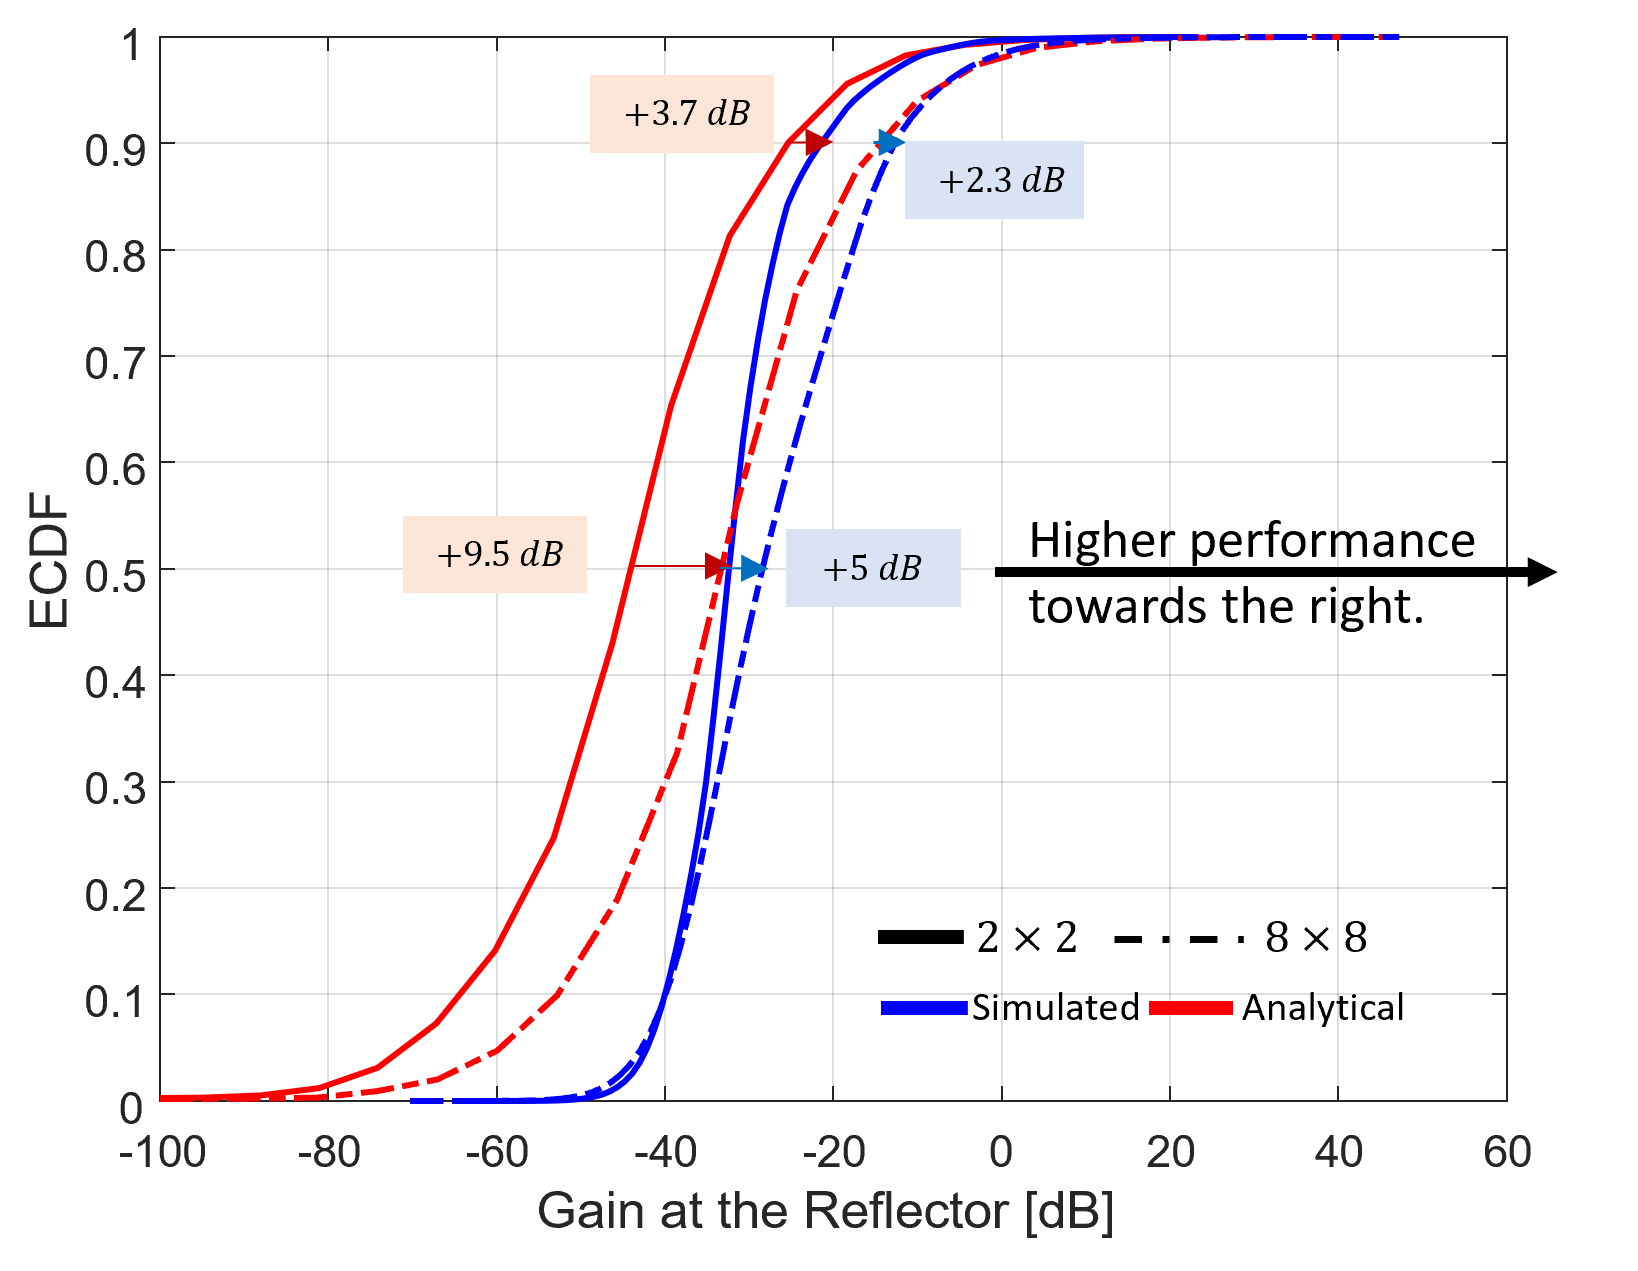
\includegraphics[width=0.7\linewidth]{images/Section 3 Images/ECDF_HELIOS_array}
	\caption{Gain vs ECDF plot for $\num{2}\times \num{2}$ and $\num{8}\times \num{8}$ HELIOS array with $a_{m,n}=b_{m,n}=\SI{10}{\centi\meter}$ for simulated and analytical results with a notable difference in gain between both the models when slope angles $\alpha_{m,n}=\beta_{m,n}=10^\circ$ with incident angles $\theta_{Tx}=\varphi_{Tx}=0^\circ$. }
	\label{fig:ECDF_HELIOS_array}
\end{figure}
Notably, for both types of HELIOS configurations, the simulation findings consistently show better performance than the analytical counterparts. Along the mean at $\num{2}\times \num{2}$ and $\num{8}\times \num{8}$ HELIOS array, the simulated results are better than the analytical model by \SI{9.5}{\decibel} and \SI{5}{\decibel} than the analytical model, whereas along the \num{90}\% quartile, the simulated results are better by \SI{3.7}{\decibel} and \SI{2.3}{\decibel}, respectively. The fact that the gain values are constantly lower shows that the analytical model avoids over-prediction. This discrepancy between the analytical and simulation results indicates a cautious approach because it suggests a conservative estimate in the analytical model. In practical applications, this careful prediction ensures that the actual performance of the system is less likely to deviate from the expected values, hence improving the analytical model's robustness and reliability. Network planning will now rather use too many reflectors or larger ones compared to not meeting the required target received signal strengths.
\subsubsection{Case Study 3: RCS Pattern Comparison for Different HELIOS Configurations and Beamwidth Factors}
The scalability needed by larger HELIOS reflectors is not met by applying \Cref{Eq:HELIOS_module} in the $\num{1}\times \num{1}$ HELIOS module. To find an ideal solution for the bigger reflector designs, we investigate and evaluate various beamwidth correction factors in order to overcome this constraint. 
One important finding from our analysis of the beamwidth correction factor for a HELIOS module is seen in \Cref{Eq:HELIOS_module} and \Cref{Table:Comparison flat plate and HELIOS}, where the correction factor is found to be $(\frac{1}{2},\frac{1}{2})$ for a HELIOS module. But when you move to an array configuration, you see a significant difference. To investigate this, we carried out a thorough analysis comprising multiple parameters, as shown in \Cref{fig:Casestudy_beamwidth} for a $\num{4}\times \num{4}$ array as well as a HELIOS module.

Referring to \Cref{Eq:HELIOS_array}, which is our final independent analytical model for the HELIOS reflector array, we vary $M/2$ and $N/2$ in both the $\sinc$ functions to change their beamwidth factor. These components include $(\frac{M}{2},\frac{N}{2})$, $(M,N)$, in addition to the previously mentioned $(\frac{1}{2},\frac{1}{2})$. 
\begin{figure}[tb]
	\centering
	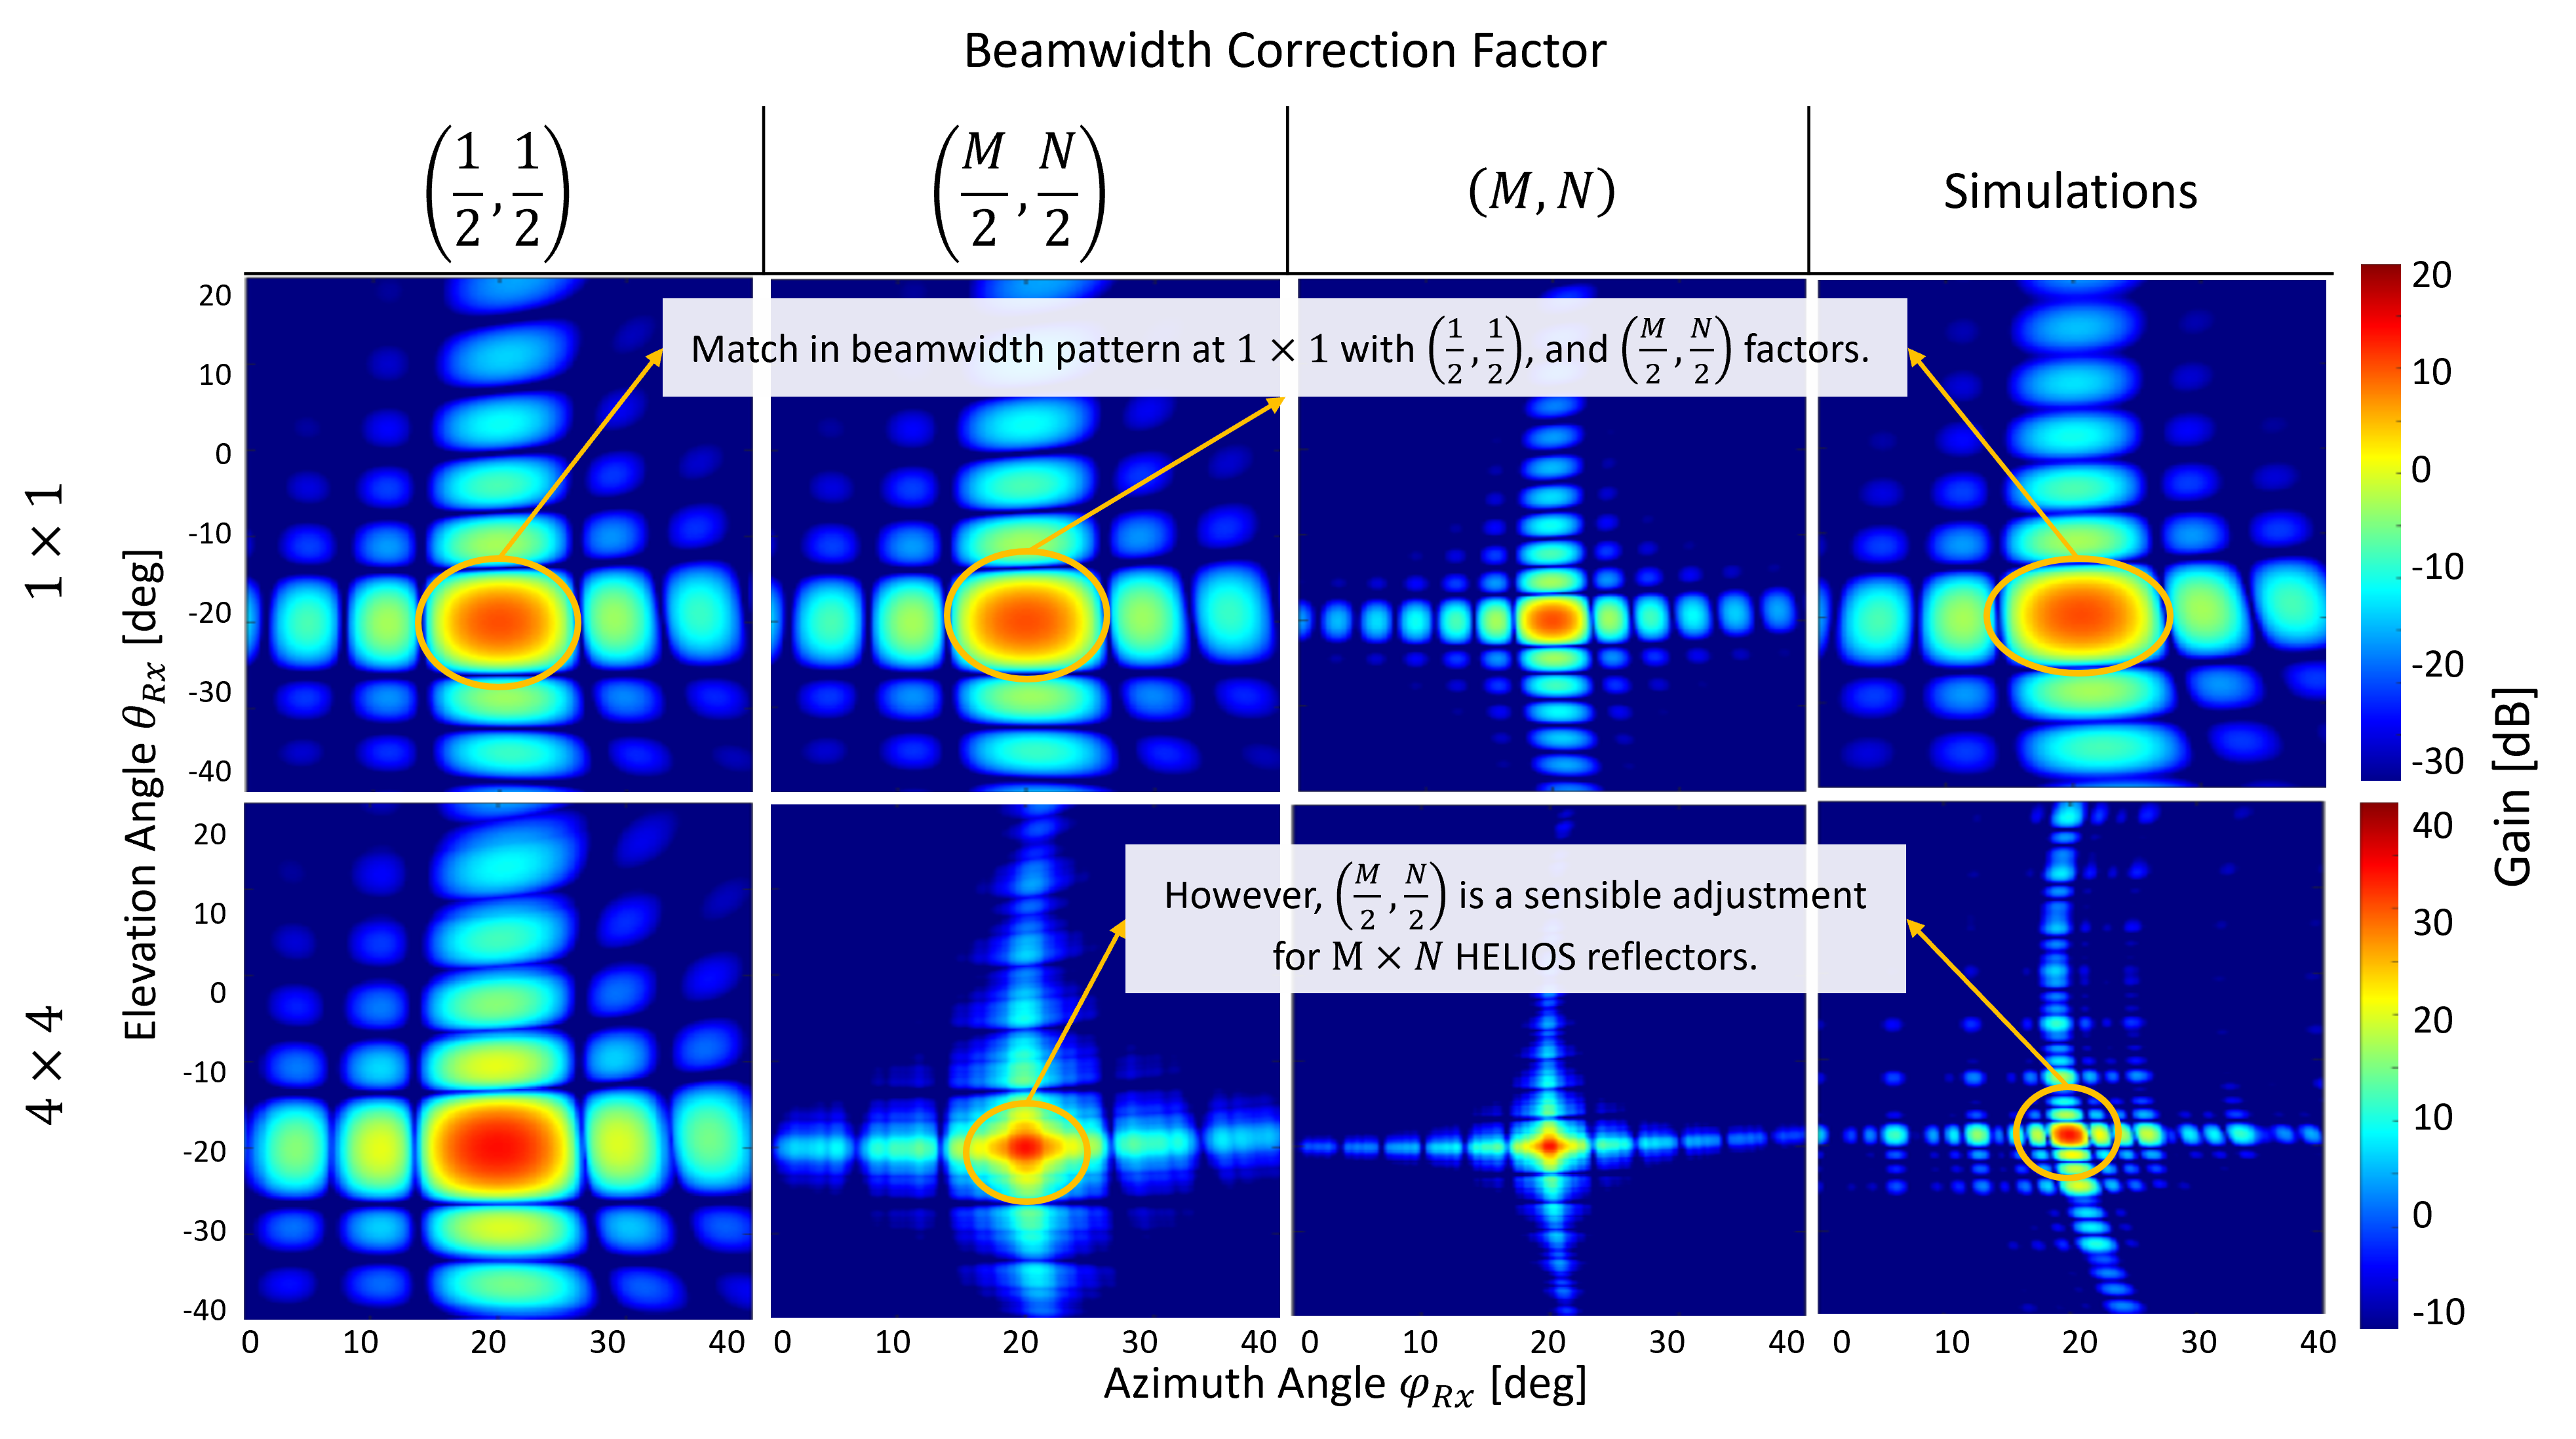
\includegraphics[width=1.0\linewidth]{images/Section 3 Images/Casestudy_beamwidth}
	\caption{Illustrating the RCS behavior of a HELIOS module and HELIOS array for different beamwidth correction factors in comparison with the simulated results when $\alpha_{m,n}=\beta_{m,n}=10^\circ$ and $a_{m,n}=b_{m,n}=\SI{10}{\centi\meter}$ for $M=N\in[1,4]$.}
	\label{fig:Casestudy_beamwidth}
\end{figure}
For the $\num{1}\times \num{1}$ and $\num{4}\times \num{4}$ HELIOS reflector array with $\alpha_{m,n}=\beta_{m,n}=10^\circ$, $a_{m,n}=b_{m,n}=\SI{10}{\centi\meter}$, and $\theta_{Tx}=\varphi_{Tx}=0^\circ$, we notice the RCS behavior in the form of heatmap in \Cref{fig:Casestudy_beamwidth}. The notable match is observed at $(\frac{M}{2},\frac{N}{2})$ and $(\frac{1}{2},\frac{1}{2})$ in the RCS heatmaps, but observing the behavior at $\num{4}\times \num{4}$ HELIOS reflector array, there's a sensible match at $(\frac{M}{2},\frac{N}{2})$.  We observe a better match in the results for larger arrays using  $(\frac{M}{2},\frac{N}{2})$ as the beamwidth correction factor.

In addition, we study a flat plate of fixed overall size by setting $\alpha_{m,n}=\beta_{m,n}=0^\circ$ with the incident wave impinging from $\theta_{Tx}=\varphi_{Tx}=0^\circ$. Like in the previous paragraph, we use the beamwidth correction factors of $(\frac{M}{2},\frac{N}{2})$, $(M,N)$, in addition to the previously mentioned $(\frac{1}{2},\frac{1}{2})$ from \Cref{Eq:HELIOS_module}. This is because we consider the same flatplate in the form of two different representations: First, as a large $\num{1}\times \num{1}$ HELIOS reflector with dimensions $a=\SI{40}{\centi\meter}$, and $b=\SI{10}{\centi\meter}$. Second, the overall plate shall be represented by four modules in the form of a $\num{1}\times \num{4}$ HELIOS with individual modules having the dimensions of $a_{m,n}=b_{m,n}=\SI{10}{\centi\meter}$. We compare the resulting overall bistatic RCS heatmaps in \Cref{fig:Casestudy_flatplate}.

In the figure below, for $1 \times 1$ large flat plate, we observe the match in the RCS heatmap behavior with beamwidth factor $(\frac{1}{2},\frac{1}{2})$, and $(\frac{M}{2},\frac{N}{2})$, whereas, for $1 \times 4$ small flat plates, the match can be observed only with beamwidth factor $(\frac{M}{2},\frac{N}{2})$. The same results were seen in \Cref{fig:Casestudy_beamwidth}, with $(\frac{M}{2},\frac{N}{2})$ as the sensible adjustment of beamwidth factor for HELIOS reflector array.
\begin{figure}[tb]
	\centering
	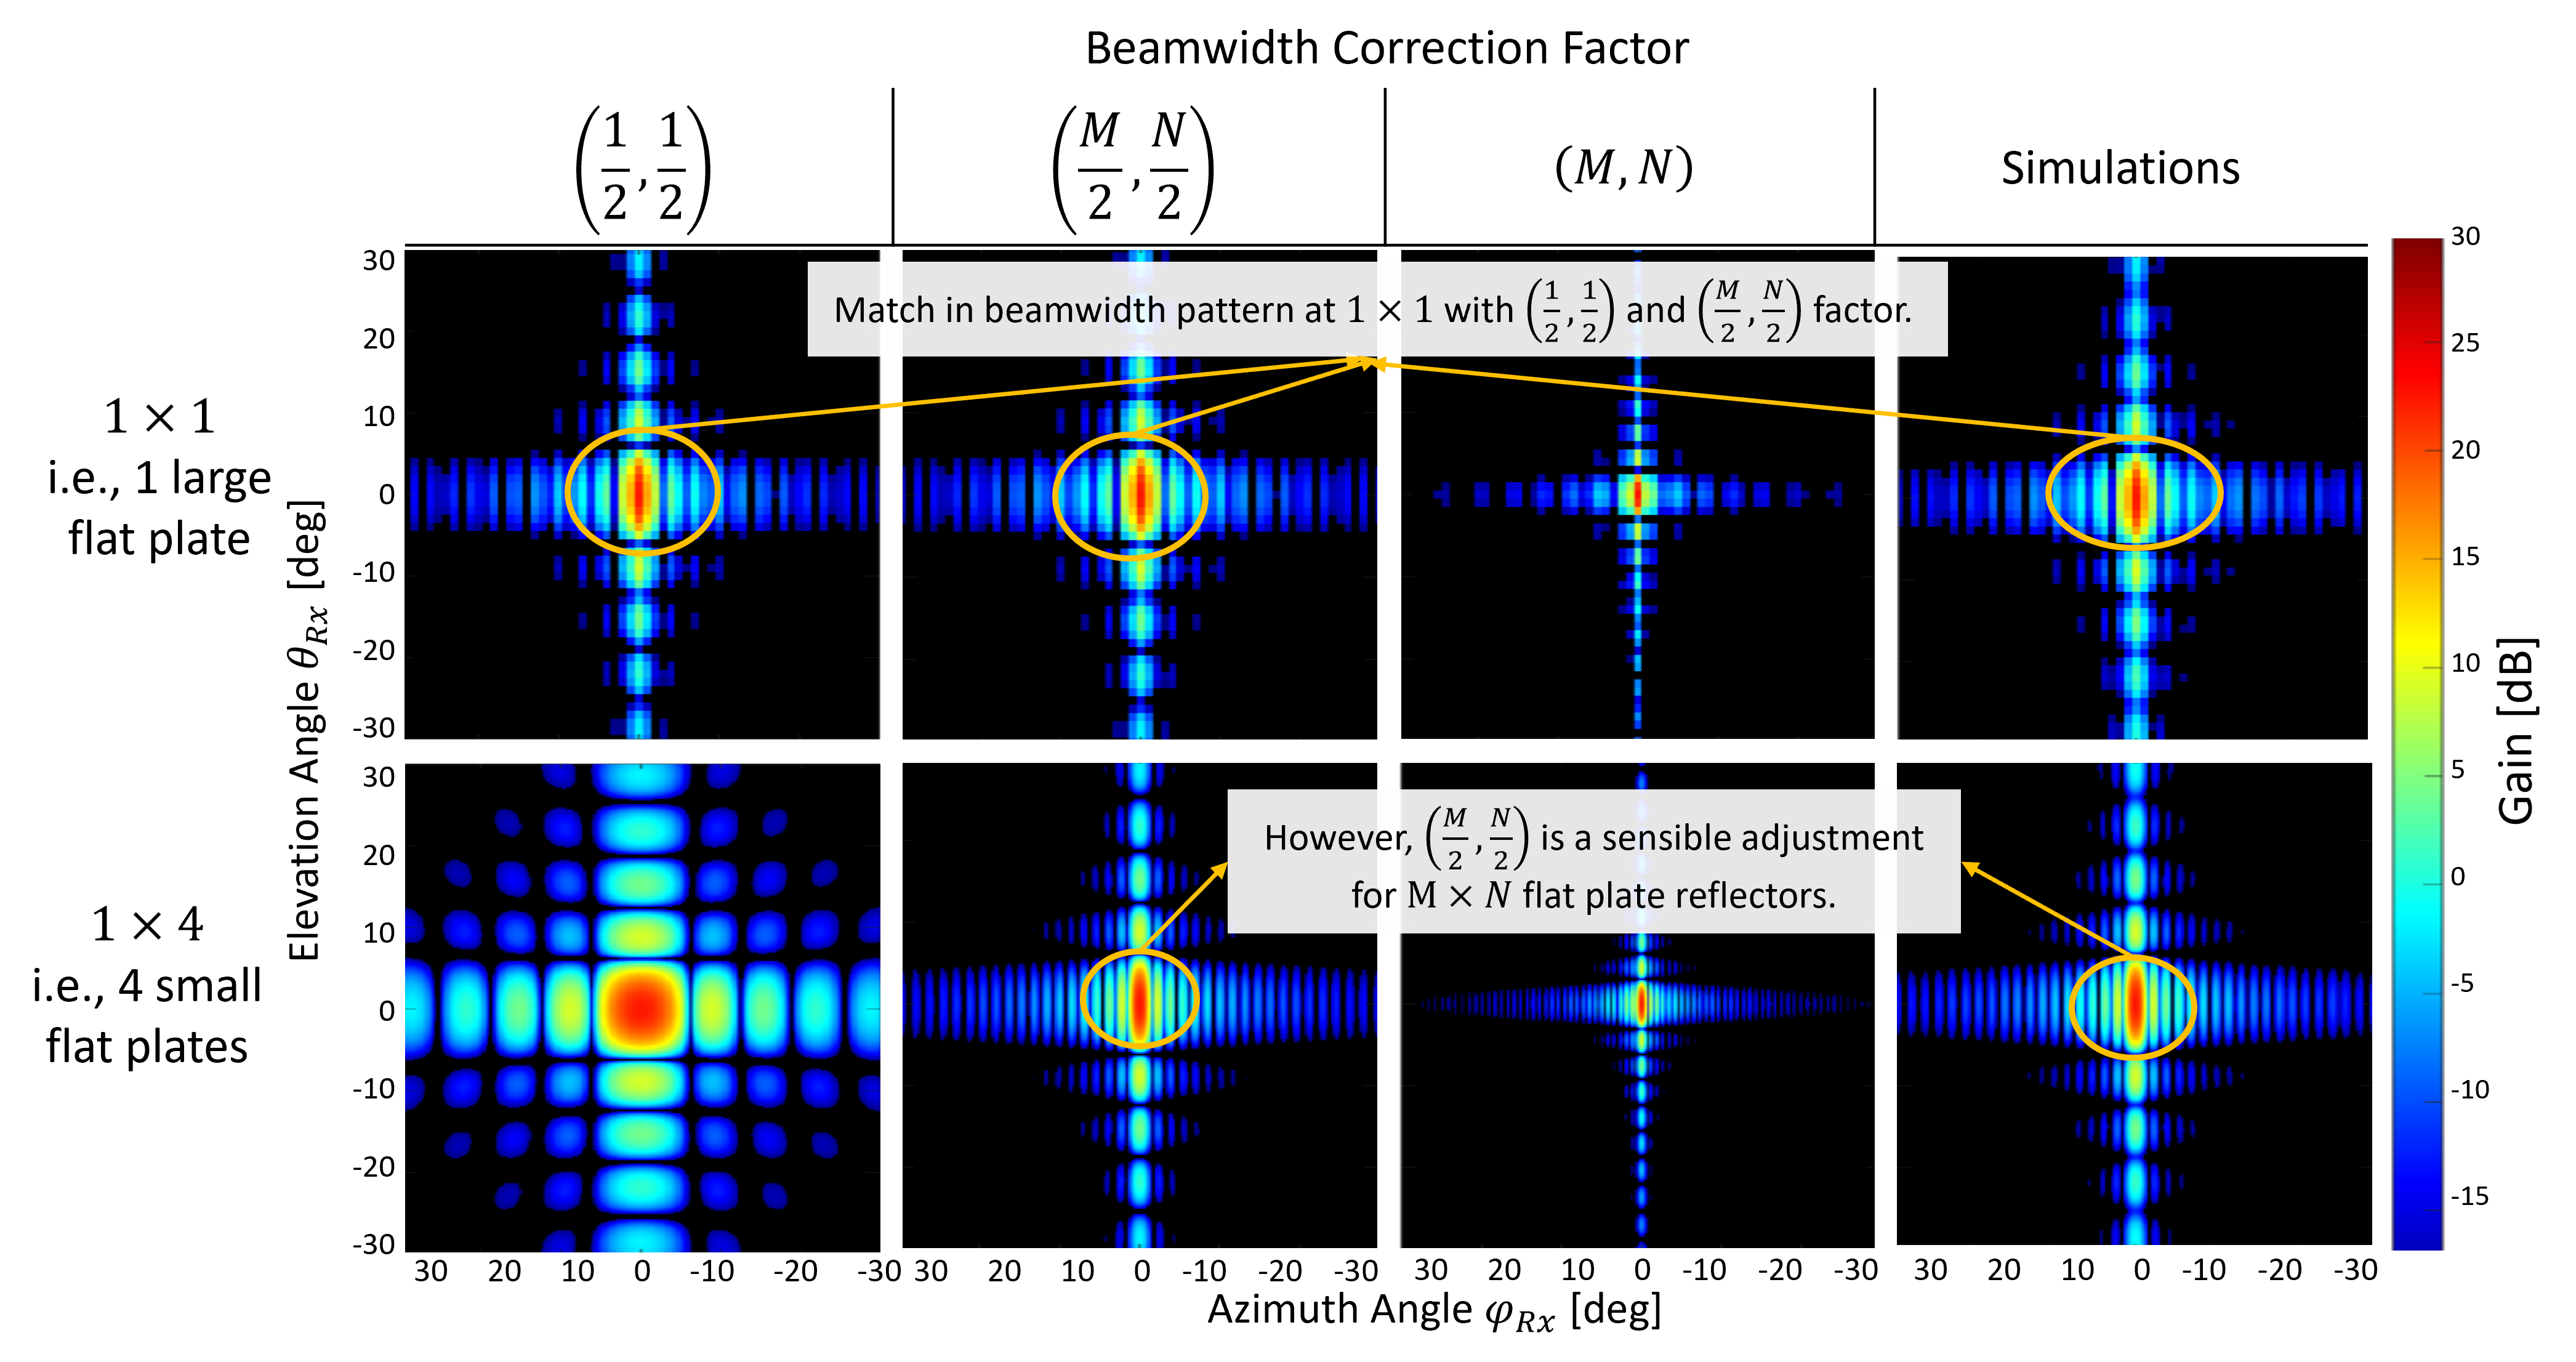
\includegraphics[width=1\linewidth]{images/Section 3 Images/Casestudy_flatplate}
	\caption{Illustrating the impact of different beamwidth correction factors in comparison with the simulations when $\alpha_{m,n}=\beta_{m,n}=0^\circ$ for a single big flat plate with $a_{m,n}=\SI{40}{\centi\meter}$, and $b_{m,n}=\SI{10}{\centi\meter}$ and multiple small flat plates with $a_{m,n}=b_{m,n}=\SI{10}{\centi\meter}$, where both the cases $1 \times 1$ and $1 \times 4$ represent the same physical plate. Notably, with beamwidth factor of $(\frac{1}{2},\frac{1}{2})$, and $(\frac{M}{2},\frac{N}{2})$, there's a match with the simulations at $1 \times 1$ , but at $1 \times 4$ HELIOS reflectors, the match is observed with beamwidth factor $(\frac{M}{2},\frac{N}{2})$.}
	\label{fig:Casestudy_flatplate}
\end{figure}
\begin{figure}[H]
	\centering
	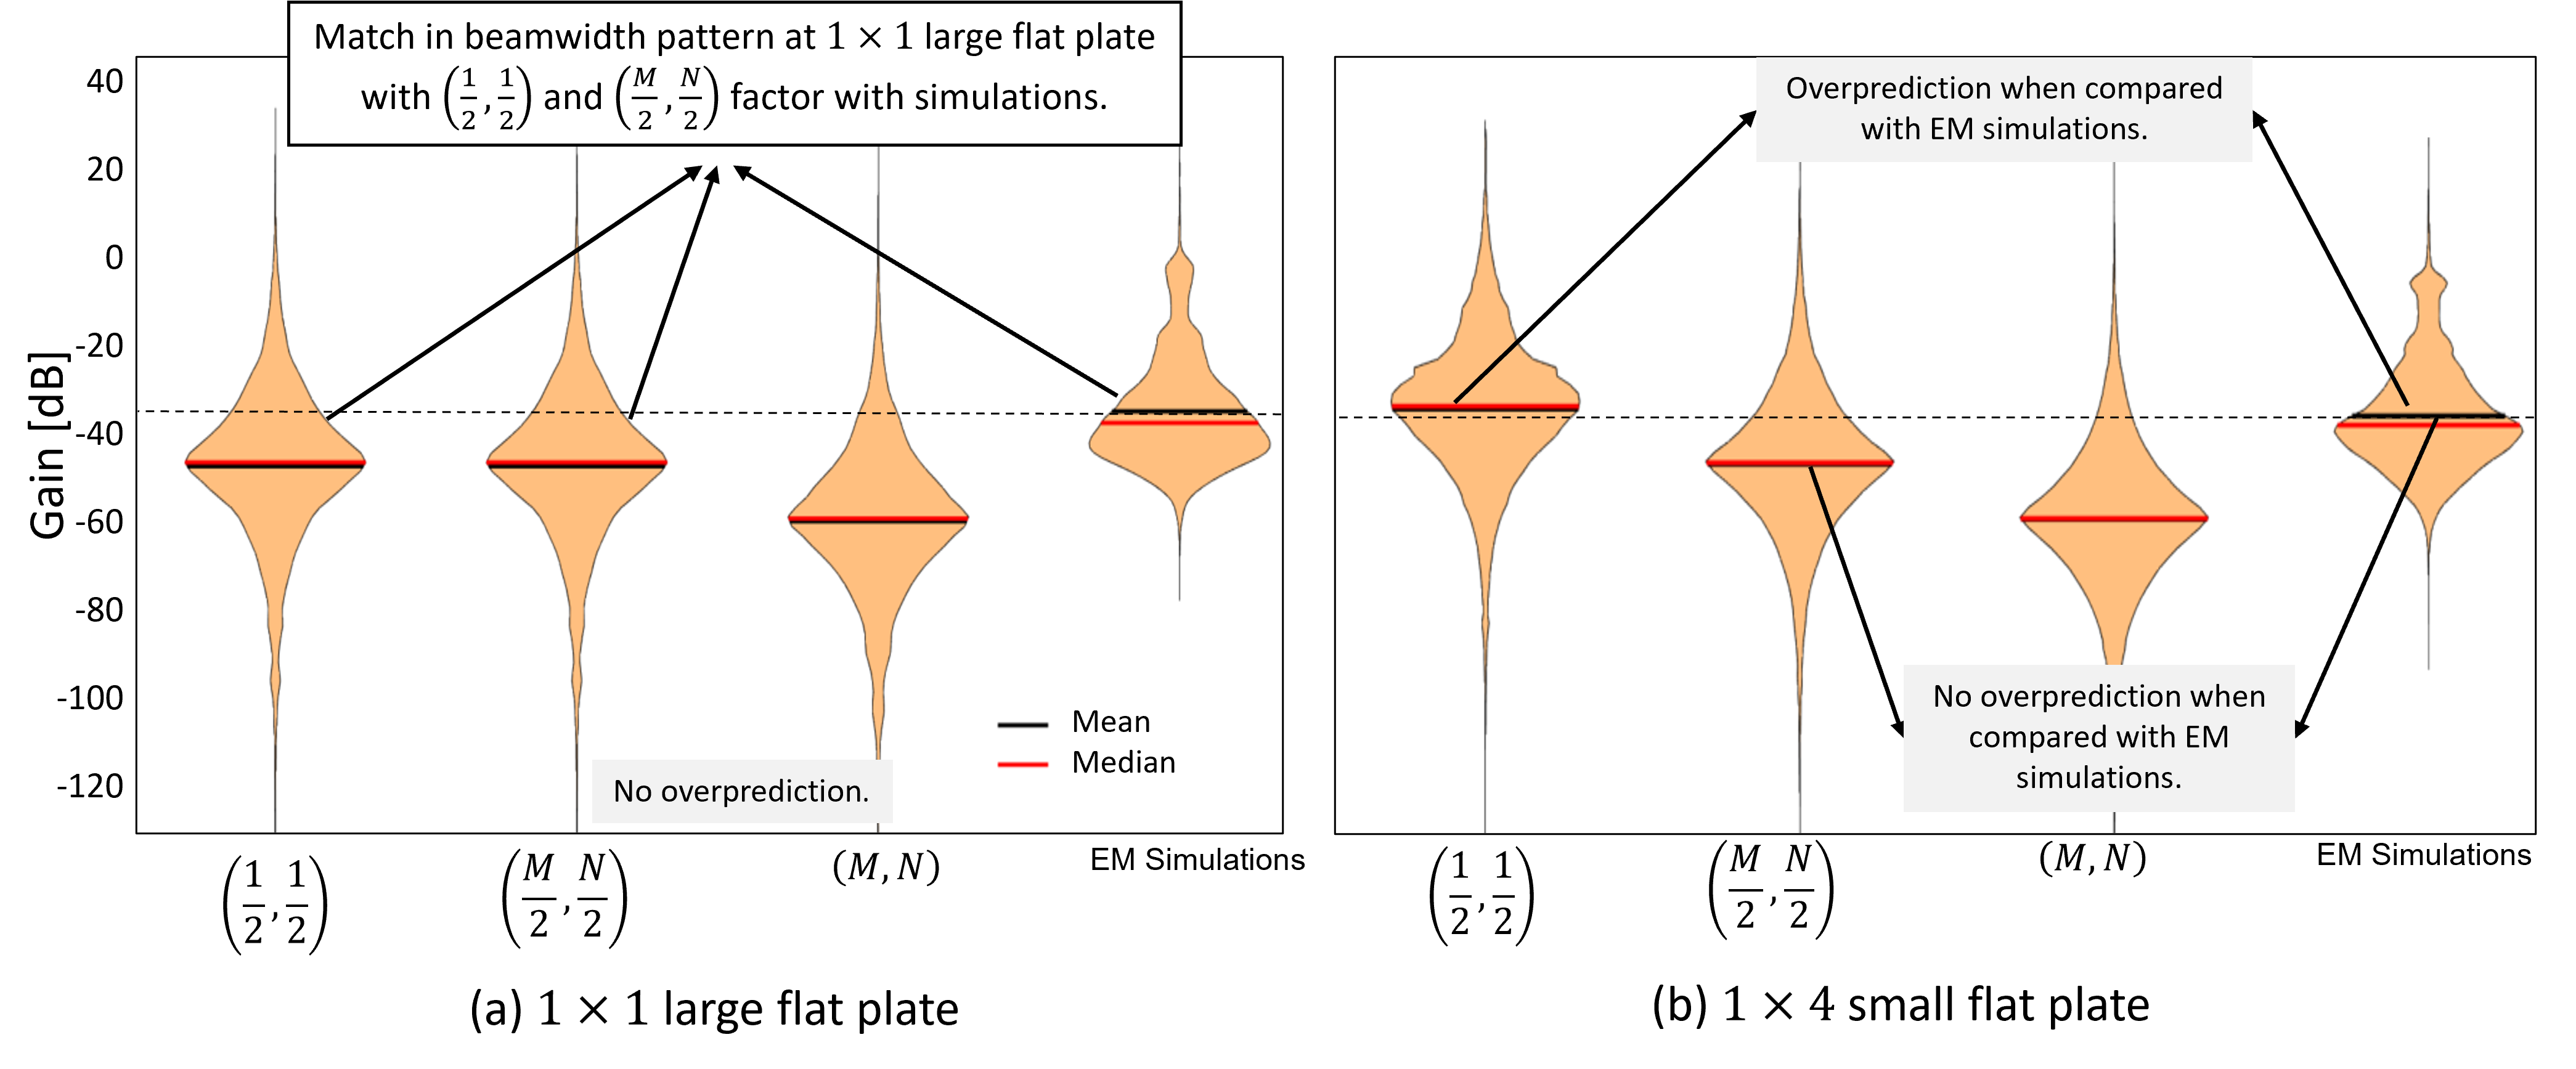
\includegraphics[width=1.0\linewidth]{images/Section 3 Images/Casestudy_flatplate_violin}
	\caption{Violin plot comparison for a flat plate scenario for different beamwidth correction factors. (a) A single big flat plate with $a_{m,n}=\SI{40}{\centi\meter}$, and $b_{m,n}=\SI{10}{\centi\meter}$, and a notable match with EM simulations with beamwidth factor of $(\frac{1}{2},\frac{1}{2})$, and $(\frac{M}{2},\frac{N}{2})$ with no overpredictions. (b) 4 small flat plates with $a_{m,n}=b_{m,n}=\SI{10}{\centi\meter}$ and a match with the simulations with beamwidth factor $(\frac{M}{2},\frac{N}{2})$ with no overpredictions. Both the cases $1 \times 1$ and $1 \times 4$ represent the same physical plate.}
	\label{fig:Casestudy_flatplate_violin}
\end{figure}
We also consider the above discussed RCS heatmaps in the form of violin plots, see \Cref{fig:Casestudy_flatplate_violin}. Notably, our analytical model regularly predicts slightly lower values, as evidenced by the mean and median values for beamwidth correction factors $(\frac{M}{2},\frac{N}{2})$, and $(M,N)$ falling below the corresponding simulation findings with both $1 \times 1$ large flat plate and $1 \times 4$ small flat plate. But when using the $(\frac{1}{2},\frac{1}{2})$ correction factor, this disparity is not seen in $1 \times 4$ small flat plate, as the model overpredicts when compared with EM simulations. Significantly, this actual data supports the analytical model and points to one of its positive features: it predicts values that are slightly lower than those obtained from simulations with beamwidth factor  $(\frac{M}{2},\frac{N}{2})$, which is in line with our intended results as argued previously.

The focus of this extended study is now to compare our analytical model with the EM simulations for a $1\times 32$ HELIOS reflector using different beamwidth correction factors. It is assumed that incidence angles are orthogonal to the backplane of the reflector, i.e., $\varphi_{Tx}=\theta_{Tx}=0^\circ$  with slope angles $\alpha_{1}=...\alpha_{32}=\num{27.6}^\circ$ and $\beta_{m,n}=0^\circ$. The overall size of the reflector shall be tuned by factor $K$ affecting the size along $y$-axis and $z$-axis, respectively, as follows: $a_{m,n}=K \cdot \frac{3}{32}$ and $b_{m,n}=K \cdot 3$ with $K = (0.1, 0.3, 0.5, 0.7)$, where $a_{m,n}$ and $b_{m,n}$ are in \si{\meter}.

\Cref{fig:Casestudy_orthogonal_BCF} provides a violin plots of $\Delta Gain$ (in \si{\decibel}) defined by $RCS_{Sim} - RCS_{Anal}$ in order to study the influence of reflector size and beamwidth correction factor on the accuracy of the model against the EM simulations. Notably, the analytical data produce mean and median values for beamwidth
\begin{figure}[H]
	\centering
	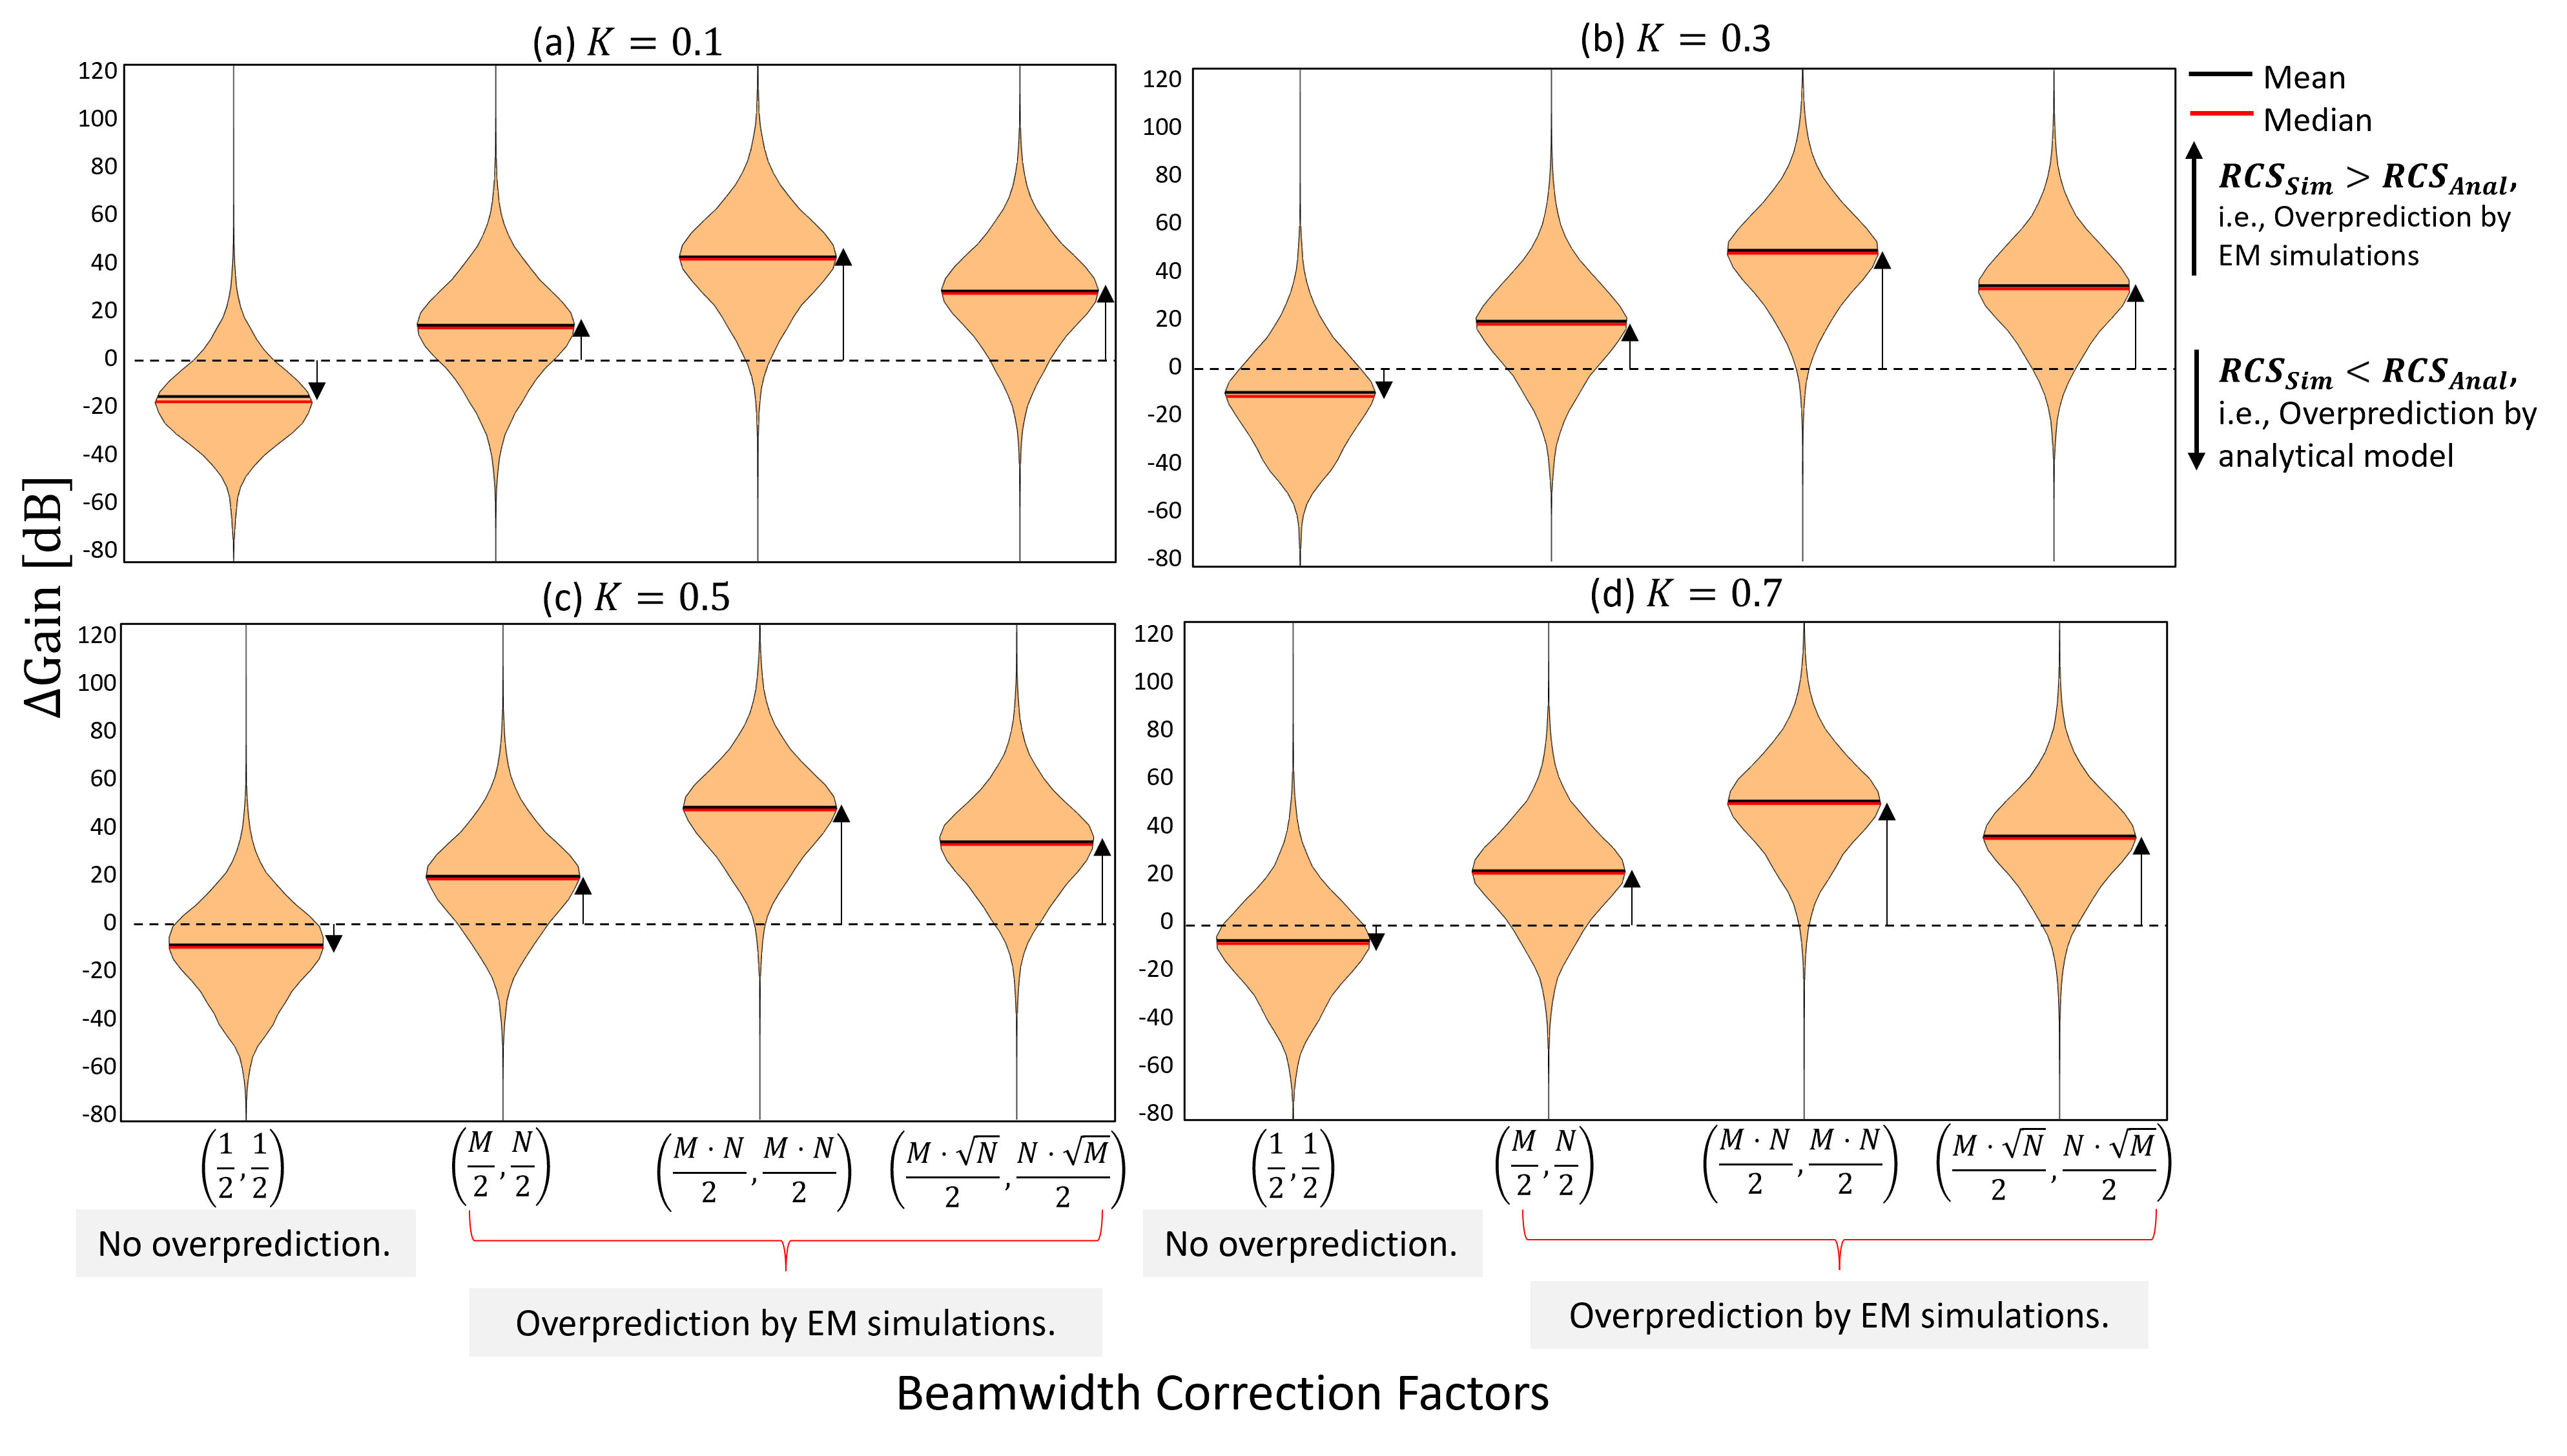
\includegraphics[width=1.0\linewidth]{images/Section 4 Images/Casestudy_orthogonal_BCF}
	\caption{Violin plots illustrating the $\Delta Gain = RCS_{Sim} - RCS_{Anal}.$ in \si{\decibel} for different beamwidth correction factors along the $x$-axis and varying HELIOS size scaling factors $K$ along the four subfigures. Here, $\varphi_{Tx}=\theta_{Tx}=0^\circ$, $\beta_1 =  \dots = \beta_{32}= 0^\circ$, and $\alpha_{1}=...\alpha_{32}=\num{27.6}^\circ$.}
	\label{fig:Casestudy_orthogonal_BCF}
\end{figure}
factors $(\frac{1}{2},\frac{1}{2})$ that are lower than those achieved from simulations, suggesting an overestimation as the mean values in all the four plots are less than zero. Whereas, our analytical model attains mean and median $\Delta Gain>\SI{0}{\decibel}$ values when using beamwidth correction factors of $(\frac{M}{2},\frac{N}{2})$, and $(\frac{M\cdot N}{2},\frac{M\cdot N}{2})$, thus suggesting little overprediction.

Assessing this along increasing $K$, we observe a gradual increase of the mean $\Delta Gain$ values, e.g., for $(\frac{1}{2},\frac{1}{2})$ they are \SI{-18.3}{\decibel}, \SI{-14.6}{\decibel}, \SI{-11.2}{\decibel} and \SI{-7.4}{\decibel}. This shows that overprediction by the analytical model in the case with beamwidth factor $(\frac{1}{2},\frac{1}{2})$ is reduced with increasing HELIOS size. The mean and median values with beamwidth factor $(\frac{M}{2},\frac{N}{2})$ has values $\Delta Gain>\SI{0}{\decibel}$, but less than that of other factors. Thus suggesting this beamwidth factor to be a sensible use for the HELIOS reflector array. 

\textbf{Additional Study: Comparative Results for Varying Reflector Size}

We continue the above case study, however, now $K$ is in range from $[0.1:3]$ \si{\meter} and we change our consideration to the one of a plat plate with $\alpha_{m,n}=\beta_{m,n}=0^\circ$ for all $n \in 1, \dots, 32 = N$ ($m=1$ due to linear array setup). We further explore the urban setting that was previously studied in this extended version, with particular emphasis on factors and assumptions pertaining to reflector properties. The underlying assumptions include an incident wave orthogonal to the reflector base  $\varphi_{Tx}=\theta_{Tx}=0^\circ$ and the prevalent usage of flat plate reflectors i.e., when $\alpha_{m,n}=\beta_{m,n}=0^\circ$. A scaling factor $K$ to determine the reflector size: $a_{m,n} = K \cdot \frac{3}{32}$, and $b_{m,n} = K$, where $K$ $ \forall [0.1:3]$ \si{\meter}. It is important to note that the total dimensions of the \num{32} reflectors preserve the equivalence $a_{m,n}=b_{m,n}$ for all $K$ values.
\begin{figure}[H]
	\centering
	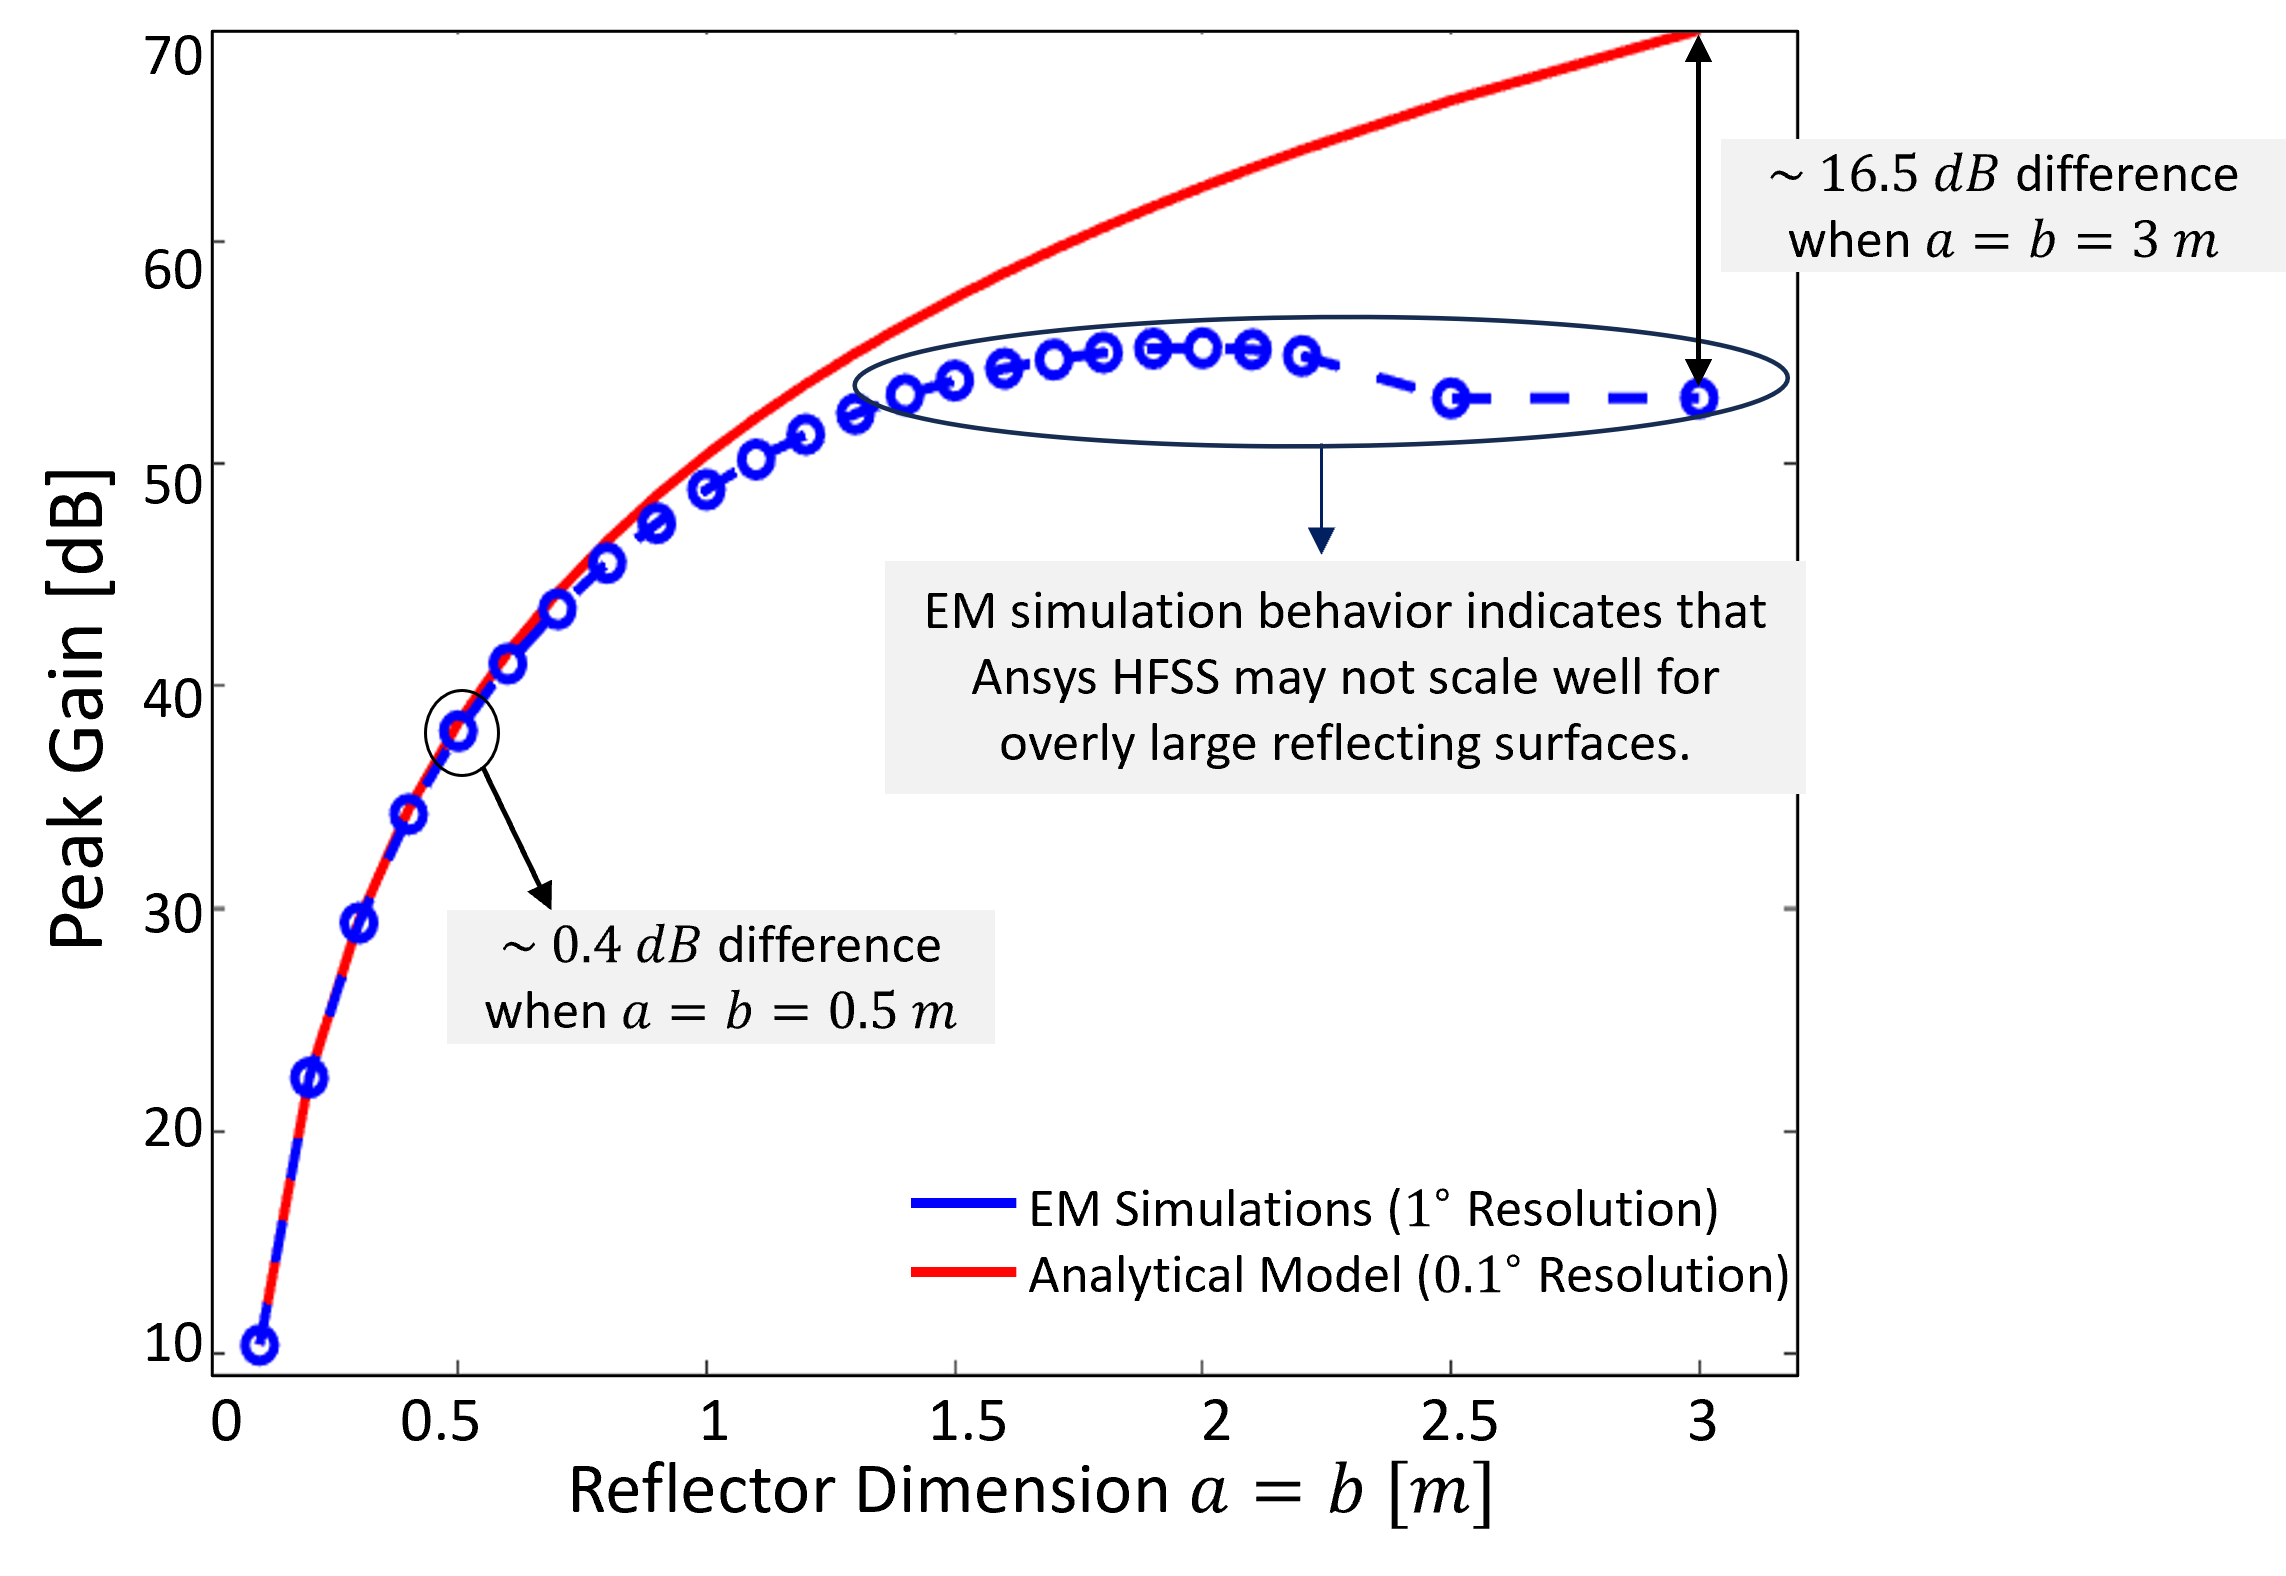
\includegraphics[width=0.8\linewidth]{images/Section 4 Images/casestudy_size}
	\caption{Comparing peak RCS value for $\varphi_{Rx}$, $\theta_{Rx} \in [-90, 90]^\circ$ range between analytical model and EM simulations along different reflecting surface size. Parameters: $\varphi_{Tx}=\theta_{Tx}=0^\circ$, $1 \times 32$ HELIOS with  $\alpha_{m,n}=\beta_{m,n}=0^\circ$ $\forall n \in 1, \dots, N$.}
	\label{fig:casestudy_size}
\end{figure}
\Cref{fig:casestudy_size} shows the peak reflection gain of EM simulations and the analytical model for different reflector sizes. The simulations were carried out with $1^\circ$ angular resolution, whereas our analytical model with $0.1^\circ$, thus, highlighting the speed and accuracy of our model. As expected, on one hand, we wind that the peak gain grows the the reflector side, cf. \Cref{Eq:HELIOS_module}. On the other hand, we observe a breakpoint in this behavior for the simulation-based result curve starting for $a_{m,n}, b_{m,n} > \SI{0.5}{\meter}$, after which the peak gain reduces. But this is not the case with our analytical model, as the model scales with the increasing reflector size directly, see \Cref{Eq:HELIOS_module}. Past this point, the models typically under estimates the rise in peak gain. For the reflector size $a_{m,n}=b_{m,n}=\SI{0.5}{\meter}$, a notable difference of about \SI{0.4}{\decibel} is observed between simulation results and our analytical model, whereas this difference increases to \SI{16.5}{\decibel} for the reflector size $a_{m,n}=b_{m,n}=\SI{3}{\meter}$.

Possible reasons for this discrepancy in the above figure by EM simulations might be reflector mismatches in their properties or a propensity for the simulation to overpredict when using bigger reflectors. It is important to recognize that situations involving huge reflector sizes may not be best handled by this particular Ansys HFSS simulation tool. In conclusion, this extended case study highlights that the findings underscore the need for examination of simulation accuracy, particularly when dealing with larger reflectors, and call for a nuanced understanding of the simulation tool's limitations in certain scenarios.
\subsection{Improved Model Using Inter-module Relations} \label{Improved Model using Inter-module Relations}
Lastly, we improve our analytical model that has been constructed successfully with the beamwidth correction factors of $(\frac{M}{2},\frac{N}{2})$ in the arguments of the respective $\sinc$ functions, cf. \Cref{Eq:HELIOS_module} and \Cref{Eq:HELIOS_array}. In the previous section, we identified that our analytical model does not yet address self-shadowing effects that may occur depending on the HELIOS configuration and the angles of arrival of the incident EM wave. To address this, we consider neighboring HELIOS modules in parts, e.g., there are $N-1$ pairs given $N$ HELIOS modules along the $y$-axis. For each pair, we then assess whether the neighboring module particularly obstruct the incident wave such that the effective reflection area becomes smaller than accounted for so far. This way, we aim to address the overprediction of the RCS peak values against the EM simulation results, as obtained in \Cref{fig:arraymax}.

\begin{figure}[tb]
	\centering
	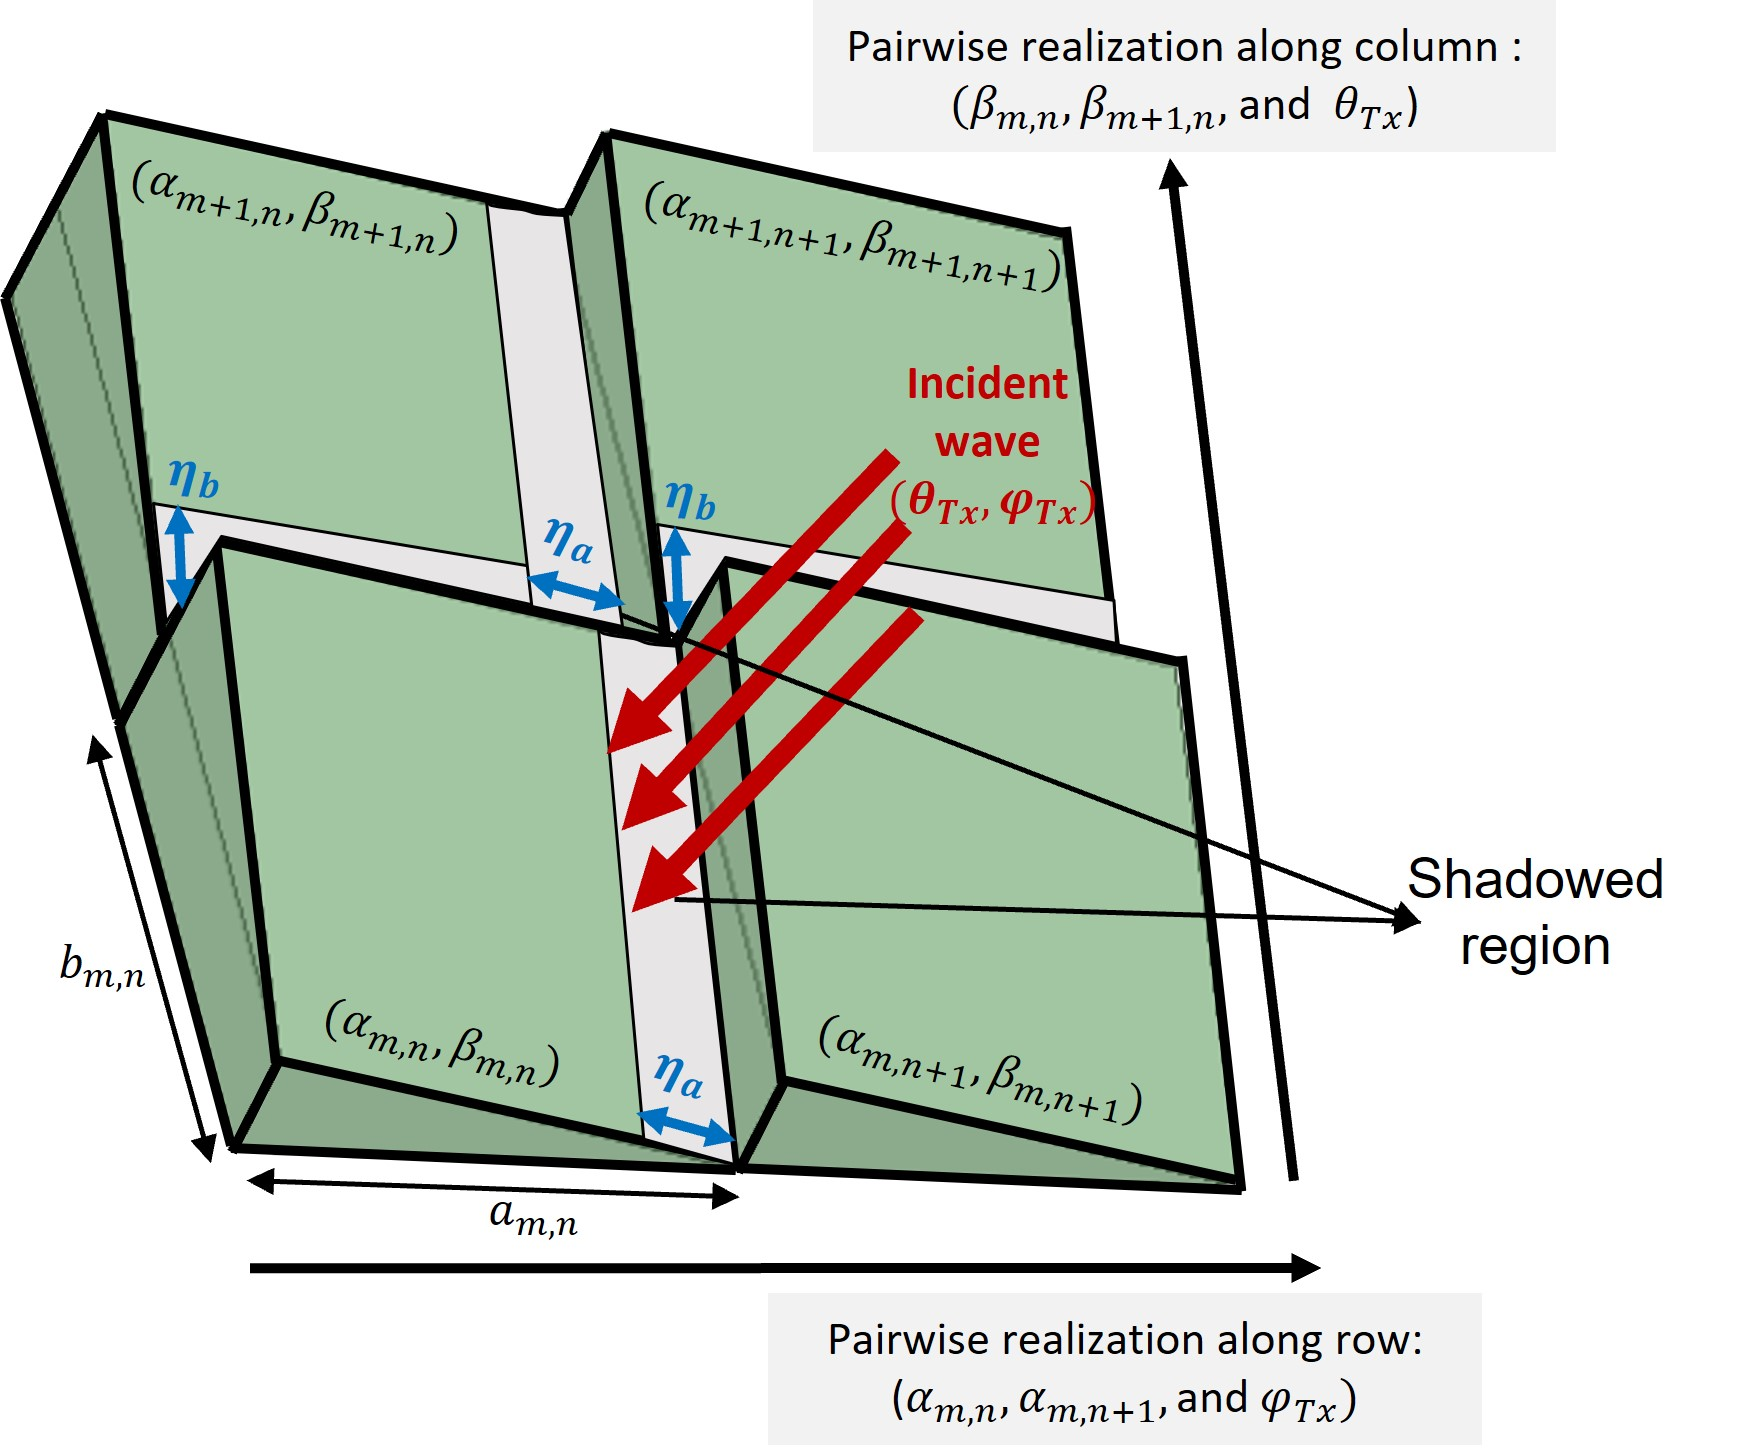
\includegraphics[width=0.65\linewidth]{images/Section 3 Images/ShadowRegion1}
	\caption{Pairwise realization of shadowing region $\eta_{a},\eta_{b}$ along $y$ and $z$ axis for incident wave $(\theta_{Tx}, \varphi_{Tx})$ along the edge for a sample HELIOS array of $2\times 2$ along row and column.}
	\label{fig:Shadow region}
\end{figure}
First, we identify the shadowed fraction of the reflecting surface area along the reflector's edge based on incidence angles $\theta_{Tx}$ and $\varphi_{Tx}$. We split our consideration of this into two parts: one where the angles $\theta_{Tx} > \num{0}^\circ $ and $\varphi_{Tx} > \num{0}^\circ$, and the other where $\theta_{Tx} \leq \num{0}^\circ $ and $\varphi_{Tx} \leq \num{0}^\circ$. We first compute the extent of the shadowed zone along the $y$-axis by taking into account the module pairs' slope angles $\alpha_{m,n}, \alpha_{m,n+1}$, and $\varphi_{Tx}$, as illustrated in \Cref{fig:Shadow region} for a $\num{2}\times \num{2}$ HELIOS reflector array. Likewise, we take into account $\beta_{m,n}, \beta_{m+1,n}$, and $\theta_{Tx}$ to determine the area that is shaded along the $z$-axis. As a result, $\eta_{a}$, and $\eta_{b}$ summarizes the shadowing along the horizontal and vertical edges of module $(m,n)$ from modules $(m,n+1)$ and $(m+1, n)$. For simplicity, we first consider the case of varying $\alpha_{m,n}$ values but with fixed $\beta_{m,n}=\num{0}^\circ$ slopes.

As thus, four separate scenarios arise, as depicted in \Cref{fig:Shadow region1}: In (a) Both the current and neighboring slope angles  values are positive i.e., $\alpha_{m,n}>0^\circ$ and $\alpha_{m,n+1}>0^\circ$. (b) Both the current and neighboring slope angles values are negative i.e., $\alpha_{m,n}<0^\circ$ and $\alpha_{m,n+1}<0^\circ$. (c) The current slope angle $\alpha_{m,n}>0^\circ$, and neighboring slope angles $\alpha_{m,n+1}<0^\circ$. (d) The current slope angle $\alpha_{m,n}<0^\circ$, and neighboring slope angles $\alpha_{m,n+1}>0^\circ$.
\begin{figure}[H]
	\centering
	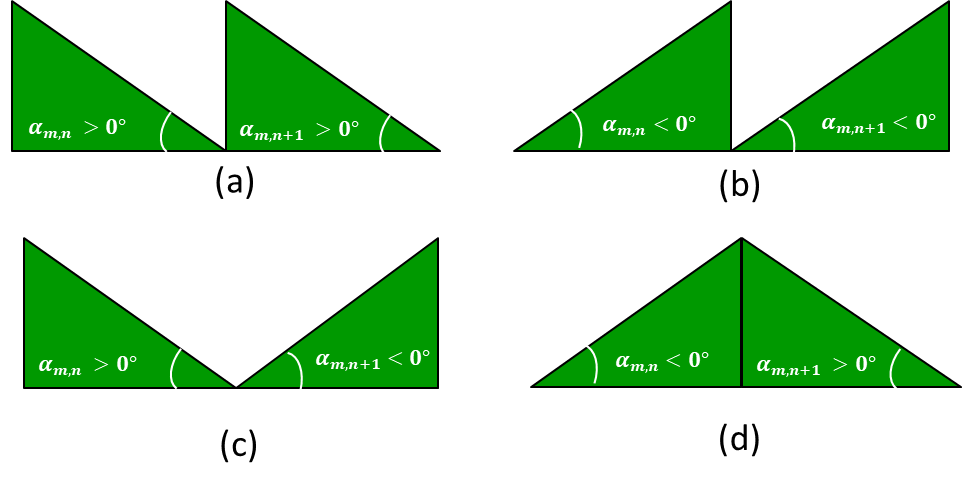
\includegraphics[width=0.85\linewidth]{images/Section 3 Images/ShadowRegion2}
	\caption{Different cases of pairwise realization for simple cases with current and neighboring slope angles $\alpha_{m,n}$, and $\alpha_{m,n+1}$. (a) Both positive slope angles (b) Both negative slope angles (c) Positive-negative slope angles (d) Negative-positive slope angles.}
	\label{fig:Shadow region1}
\end{figure}
This thorough investigation establishes the foundation for deciphering the complex interaction of factors. The calculations of shadowing factors $\eta_{a_{m,n}}$, and $\eta_{b_{m,n}}$ take into account different incident angles cases, i.e., $\theta_{Tx} > \num{0}^\circ $ and $\varphi_{Tx} > \num{0}^\circ$ and also the case when $\theta_{Tx} \leq \num{0}^\circ $ and $\varphi_{Tx} \leq \num{0}^\circ$. To fully comprehend the behavior of the model under various settings, these varied scenarios, see \Cref{fig:Shadow region1} must be included. In particular, because of the way we approached pairwise realization, our tables in \Cref{Table:Shadow region along the row} and \Cref{Table:Shadow region along the column} include formulas for both reflectors, i.e., $\alpha_{m,n}, \alpha_{m,n+1}$ along the row and $\beta_{m,n}, \beta_{m+1,n}$ along the column. \Cref{fig:shadow_derivation} considers the case for the incident angles $\theta_{Tx}=\num{0}^\circ$, and $\varphi_{Tx}>\num{0}^\circ$ and the slope angles $\alpha_{m,n}$, and $\alpha_{m,n+1}$ are positive with $a_{m,n}$ and $a_{m,n+1}$ being the dimension of current and neighboring model. The figure helps in the derivation of the shadowing factor $\eta_{a_{m,n}}$ for this particular case. 

The shadowing factor $\eta_{a_{m,n}}$ from the figure can be derived using the law of sine in the blue shaded triangle. For this particular case, the equation follows as such:
\begin{equation} \label{eq:shadowfactor}
	\frac{\sin(\varphi_{Rx})}{\eta_{a_{m,n}}}=\frac{\sin(90^\circ-\varphi_{Rx}+\alpha_{m,n})}{h_{m,n+1}},
\end{equation}
where $h_{m,n+1}$ is the height of the neighboring reflector given by
\begin{equation}
	h_{m,n+1}= a_{m,n+1} \cdot \tan(\alpha_{m,n+1}).
\end{equation}
The shadowing factor $\eta_{a_{m,n}}$ can be extracted from \Cref{eq:shadowfactor} as
\begin{equation}
	\eta_{a_{m,n}}=h_{m,n+1} \cdot \frac{\sin(\varphi_{Rx})}{\sin(90^\circ-\varphi_{Rx}+\alpha_{m,n})}.
\end{equation}
Similarly, the derivation is considered for different cases in \Cref{fig:Shadow region1} and different incident angles. The derivation of shadow factor $\eta_{b_{m,n}}$ is carried out considering $\theta_{Tx}, \beta_{m,n}, \beta_{m+1,n}, b_{m,n}$, and $b_{m,n+1}$ when $\varphi_{Tx}=0^\circ$. 
\begin{figure}[H]
	\centering
	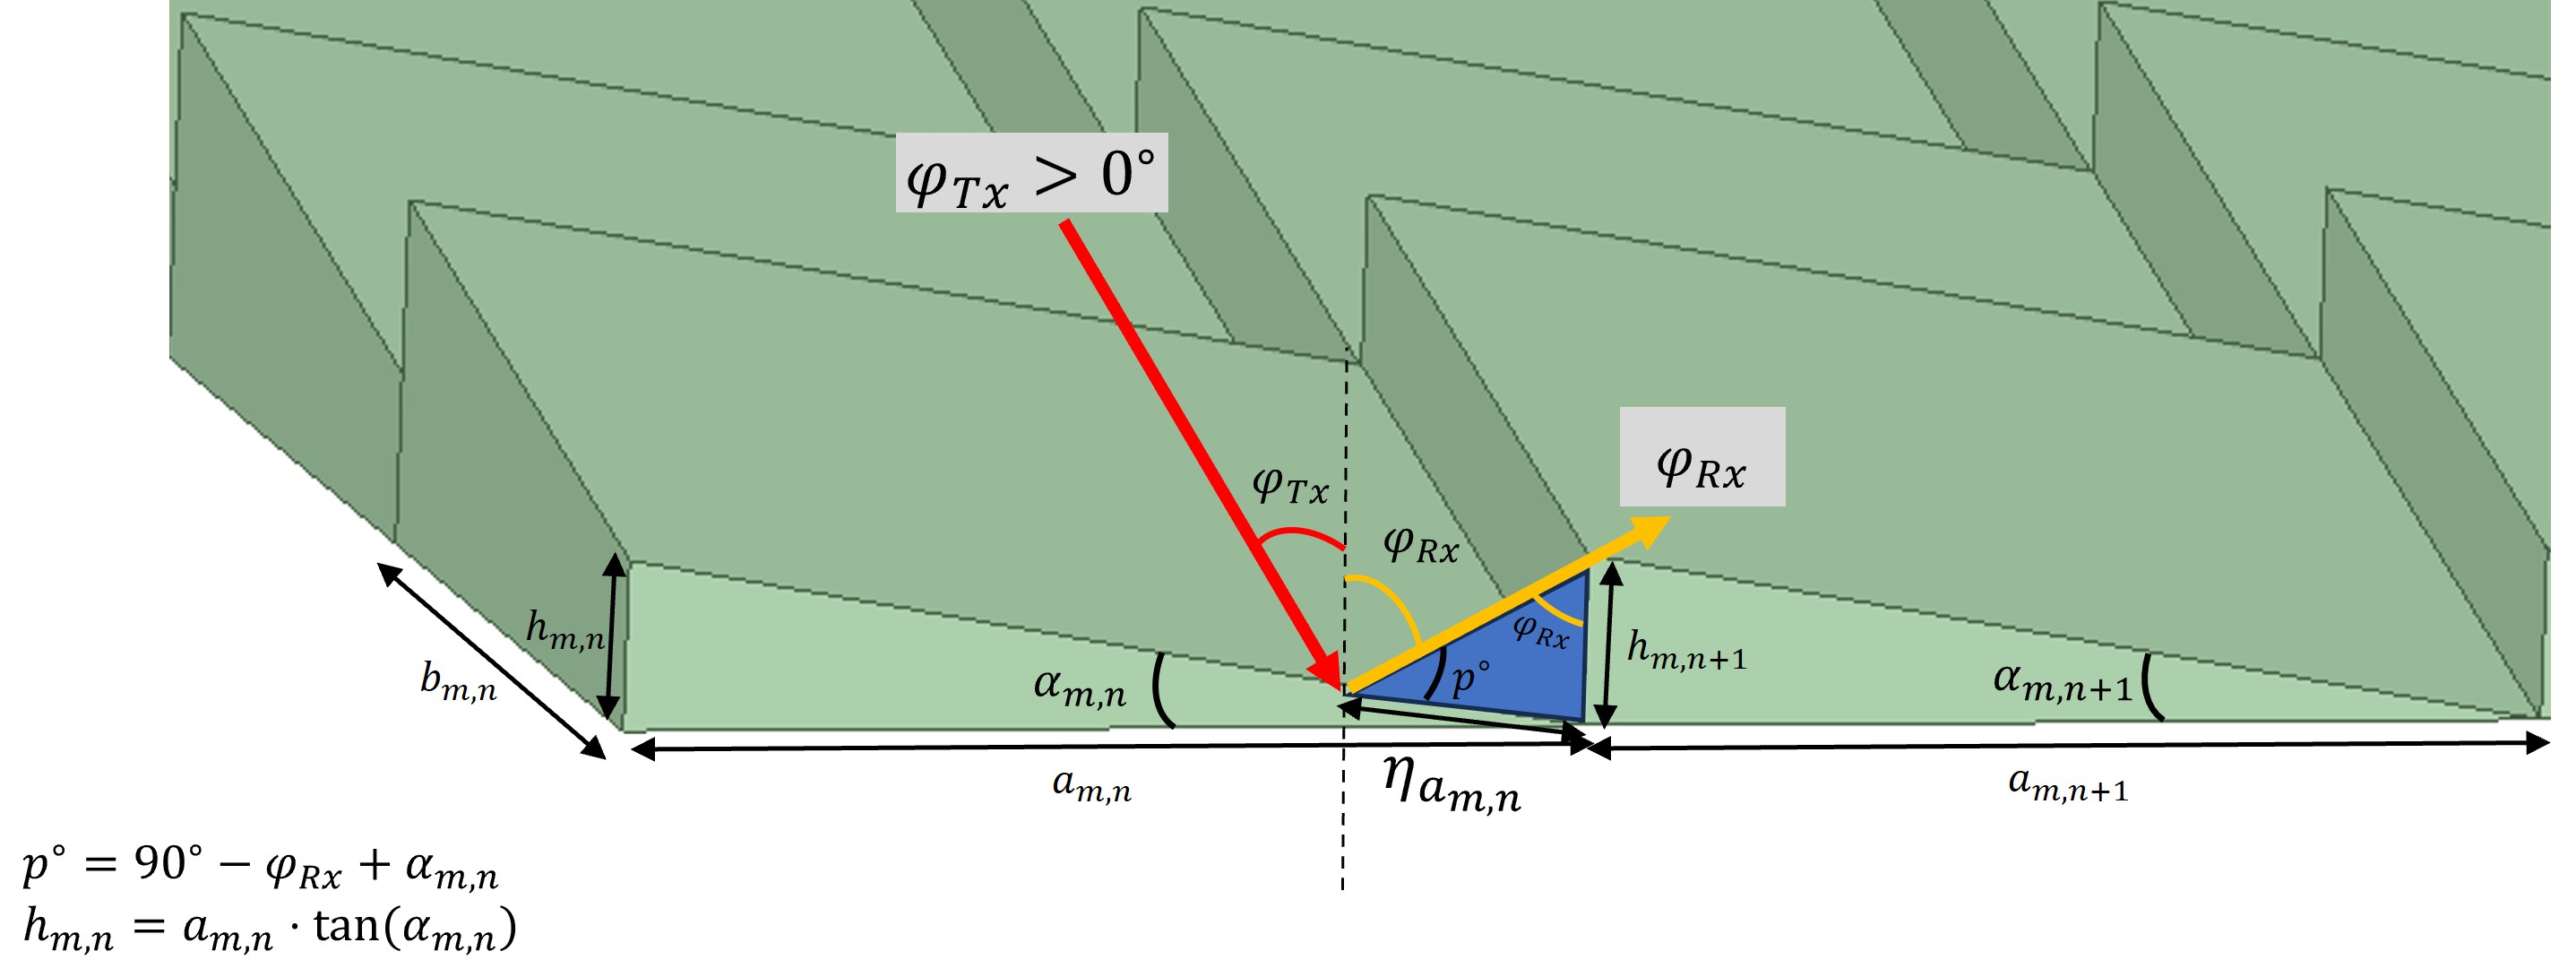
\includegraphics[width=1\linewidth]{images/Section 3 Images/shadow_derivation}
	\caption{Depiction of the shadowing factor $\eta_{a_{m,n}}$ for the case when the incident angles $\theta_{Tx}=\num{0}^\circ$,  $\varphi_{Tx}>\num{0}^\circ$ and the slope angles $\alpha_{m,n}$, and $\alpha_{m,n+1}$ are positive with $a_{m,n}$ and $a_{m,n+1}$. Here, $h_{m,n}$ and $h_{m,n+1}$ are the heights of the current and neighboring reflectors. }
	\label{fig:shadow_derivation}
\end{figure}
Using the shadowing factors $\eta_{a_{m,n}}$, and $\eta_{b_{m,n}}$ for the current and neighboring reflector with $m$ and $n$ indices, the \Cref{Table:Shadow region along the row} and \Cref{Table:Shadow region along the column} provides a detailed presentation of the obtained derived formulas for the shadowed region along the rows and columns, respectively.

We determine the effective reflecting surface size $a_{m,n}^* \times b_{m,n}^*$ as shown in \Cref{Eq:effective region_a} and \Cref{Eq:effective region_b}.
\begin{equation} \label{Eq:effective region_a}
	a_{m,n}^*= (1-\eta_{a_{m,n}})\cdot a_{m,n}
\end{equation}
\begin{equation} \label{Eq:effective region_b}
	b_{m,n}^*= (1-\eta_{b_{m,n}})\cdot b_{m,n}
\end{equation}
 Here, $\eta_{a_{m,n}}$ is for pairwise realization of model along the row, whereas $\eta_{b_{m,n}}$ is along the column.
 
\begin{table}[H] % H -> dieses objekt wird genau da wo der code steht festgenagelt
	\footnotesize
	\caption{Shadowed region for the first reflector along the row and column for cases in \Cref{fig:Shadow region1}. }
	\label{Table:Shadow region along the row}
	\centering
	\begin{tabular}{c|c|c}
	\textbf{Slope Angle} & \textbf{Incident} & \textbf{Shadowing Factor Formulae at the First Reflector}\\
	\hline
	\multirow{2}{*}{\begin{tabular}{@{}c@{}c@{}c@{}}$\alpha_{m,n}>0^\circ $\\ $\alpha_{m,n+1}>0^\circ $ \\ $\beta_{m,n}>0^\circ $\\ $\beta_{m+1,n}>0^\circ $ \end{tabular}}
	& 
	\begin{tabular}{@{}c@{}} $\varphi_{Tx}>0^\circ $ \\ $\theta_{Tx}>0^\circ $ \end{tabular}
	&
	\begin{math} \label{eq:1:SR}
		\begin{aligned}
			\eta_{a_{m,n}} &= \frac{a_{m,n+1}}{a_{m,n}} \cdot \tan(\alpha_{m,n+1}) \cdot \frac{\sin(\varphi_{Tx})}{\cos(-\varphi_{Tx}+ \alpha_{m,n})}, \varphi_{Tx}>0^\circ \\
			\eta_{b_{m,n}} &= 0, \theta_{Tx} >0^\circ \\
		\end{aligned}		
	\end{math}\\
	\cline{2-3}
	& 
	\begin{tabular}{@{}c@{}}$\varphi_{Tx} \leq 0^\circ $ \\ $\theta_{Tx} \leq 0^\circ $ \end{tabular}
	&
	\begin{math}\label{eq:2:SR}
		\begin{aligned}
			\eta_{a_{m,n}} &=
			\begin{cases}
				\frac{a_{m,n+1}}{a_{m,n}} \cdot \tan(\alpha_{m,n+1}) \cdot \frac{\sin(-\varphi_{Tx}+ 2\cdot \alpha_{m,n+1})}{\cos(-\varphi_{Tx}+ \alpha_{m,n}-2 \cdot \alpha_{m,n+1})}, &  \varphi_{Tx} > -90^\circ + \alpha_{m,n} \\
				1, & \varphi_{Tx} < -90^\circ + \alpha_{m,n} \\
			\end{cases}\\
			\eta_{b_{m,n}} &=
			\begin{cases}
				0, & \theta_{Tx} >-90^\circ + \beta_{m+1,n}\\
				1, & \theta_{Tx} < -90^\circ + \beta_{m+1,n}\\
			\end{cases}
		\end{aligned}		
	\end{math}\\
	\hline
	\multirow{2}{*}{\begin{tabular}{@{}c@{}c@{}c@{}}$\alpha_{m,n}<0^\circ $\\ $\alpha_{m,n+1}<0^\circ $ \\ $\beta_{m,n}<0^\circ $\\ $\beta_{m+1,n}<0^\circ $ \end{tabular}}
	& 
	\begin{tabular}{@{}c@{}}$\varphi_{Tx}>0^\circ $ \\ $\theta_{Tx}>0^\circ $ \end{tabular}
	&
	\begin{math}
		\begin{aligned}
			\eta_{a_{m,n}} &=
			\begin{cases}
				0, & \varphi_{Tx} < 90^\circ + \alpha_{m,n}\\
				1, & \varphi_{Tx} > 90^\circ + \alpha_{m,n}\\
			\end{cases}\\
			\eta_{b_{m,n}} &=
			\begin{cases}
				\frac{b_{m+1,n}}{b_{m,n}} \cdot \tan(\beta_{m+1,n}) \cdot \frac{\sin(-\theta_{Tx}+2 \cdot \beta_{m,n})}{\cos(-\theta_{Tx}-2 \cdot \beta_{m,n}+ \beta_{m+1,n})}, &  \theta_{Tx} < 90^\circ + \beta_{m,n} \\
				1, & \theta_{Tx} > 90^\circ + \beta_{m,n} \\
			\end{cases}\\
		\end{aligned}		
	\end{math}\\
	\cline{2-3}
	& 
	\begin{tabular}{@{}c@{}}$\varphi_{Tx} \leq 0^\circ $ \\ $\theta_{Tx} \leq 0^\circ $ \end{tabular}
	&
	\begin{math}
		\begin{aligned}
			\eta_{a_{m,n}} &= 0, \varphi_{Tx} < 0^\circ \\
			\eta_{b_{m,n}} &= \frac{b_{m+1,n}}{b_{m,n}} \cdot \tan(\beta_{m+1,n}) \cdot \frac{\sin(\theta_{Tx})}{\cos(-\theta_{Tx}+ \beta_{m,n})}, \theta_{Tx} < 0^\circ \\
		\end{aligned}		
	\end{math}\\
	\hline
	\multirow{2}{*}{\begin{tabular}{@{}c@{}c@{}c@{}}$\alpha_{m,n}>0^\circ $\\ $\alpha_{m,n+1}<0^\circ $ \\ $\beta_{m,n}>0^\circ $\\ $\beta_{m+1,n}<0^\circ $ \end{tabular}}
	& 
	\begin{tabular}{@{}c@{}}$\varphi_{Tx}>0^\circ $ \\ $\theta_{Tx}>0^\circ $ \end{tabular}
	&
	\begin{math}
		\begin{aligned}
			\eta_{a_{m,n}} &=
			\begin{cases}
				0, & \varphi_{Tx} < 90^\circ + \alpha_{m,n+1}\\
				\frac{a_{m,n+1}}{a_{m,n}}\sqrt{1+ \tan^2 (\alpha_{m,n+1})} \frac{\sin(\varphi_{Tx}+ \alpha_{m,n+1}- 90^\circ)}{\cos(-\varphi_{Tx}+ \alpha_{m,n})}, &\varphi_{Tx} > 90^\circ + \alpha_{m,n+1}\\
			\end{cases}\\
			\eta_{b_{m,n}} &=
			\begin{cases}
				0, & \theta_{Tx} < 90^\circ + \beta_{m,n}\\
				1, & \theta_{Tx} > 90^\circ + \beta_{m,n}\\
			\end{cases}\\
		\end{aligned}		
	\end{math}\\
	\cline{2-3}
	& 
	\begin{tabular}{@{}c@{}}$\varphi_{Tx} \leq 0^\circ $ \\ $\theta_{Tx} \leq 0^\circ $ \end{tabular}
	&
	\begin{math}
		\begin{aligned}
			\eta_{a_{m,n}} &=
			\begin{cases}
				0, & \varphi_{Tx} > -90^\circ + \alpha_{m,n}\\
				1, & \varphi_{Tx} < -90^\circ + \alpha_{m,n}\\
			\end{cases}\\
			\eta_{b_{m,n}} &=
			\begin{cases}
				0, & \theta_{Tx} > -90^\circ + \beta_{m+1,n}\\
				\frac{b_{m+1,n}}{b_{m,n}}\sqrt{1+ \tan^2 (\beta_{m+1,n})} \frac{\sin(\theta_{Tx}+ \beta_{m+1,n}- 90^\circ)}{\cos(-\theta_{Tx}+ \beta_{m,n})}, & \theta_{Tx} < -90^\circ + \beta_{m+1,n}\\
			\end{cases}\\
		\end{aligned}		
	\end{math}\\
	\hline
	\multirow{2}{*}{\begin{tabular}{@{}c@{}c@{}c@{}}$\alpha_{m,n}<0^\circ $\\ $\alpha_{m,n+1}>0^\circ $ \\ $\beta_{m,n} <0^\circ $\\ $\beta_{m+1,n}>0^\circ $ \end{tabular}}
	& 
	\begin{tabular}{@{}c@{}}$\varphi_{Tx}>0^\circ $ \\ $\theta_{Tx}>0^\circ $ \end{tabular}
	&
	\begin{math}
		\begin{aligned}
			\eta_{a_{m,n}} &=
			\begin{cases}
				0, & \varphi_{Tx} < 90^\circ - \alpha_{m,n+1}\\
				1, & \varphi_{Tx} > 90^\circ - \alpha_{m,n+1}\\
			\end{cases}\\
			\eta_{b_{m,n}} &= 0, \theta_{Tx} > 0^\circ\\
		\end{aligned}		
	\end{math}\\
	\cline{2-3}
	& 
	\begin{tabular}{@{}c@{}}$\varphi_{Tx} \leq 0^\circ $ \\ $\theta_{Tx} \leq 0^\circ $ \end{tabular}
	&
	\begin{math}
		\begin{aligned}
			\eta_{a_{m,n}} &= 0,   \varphi_{Tx} > 0^\circ\\
			\eta_{b_{m,n}} &=
			\begin{cases}
				0, & \theta_{Tx} > -90^\circ + \beta_{m+1,n}\\
				1, & \theta_{Tx} < -90^\circ + \beta_{m+1,n}\\
			\end{cases}
		\end{aligned}		
	\end{math}
	\end{tabular}
\end{table}
\begin{table}[tb] % H -> dieses objekt wird genau da wo der code steht festgenagelt
		\footnotesize
	\caption{Shadowed region for the second reflector along the row and column for cases in \Cref{fig:Shadow region1}.}
	\label{Table:Shadow region along the column}
	\centering
	\begin{tabular}{c|c|c}
		\textbf{Slope Angle} & \textbf{Incident} & \textbf{Shadowing Factor Formulae at the Second Reflector}\\
		\hline
		\multirow{2}{*}{\begin{tabular}{@{}c@{}c@{}c@{}}$\alpha_{m,n}>0^\circ $\\ $\alpha_{m,n+1}>0^\circ $ \\ $\beta_{m,n}>0^\circ $\\ $\beta_{m+1,n}>0^\circ $ \end{tabular}}
		& 
		\begin{tabular}{@{}c@{}}$\varphi_{Tx}>0^\circ $ \\ $\theta_{Tx}>0^\circ $ \end{tabular}
		&
		\begin{math}
			\begin{aligned}
				\eta_{a_{m,n+1}} &= 0, \varphi_{Tx} >0^\circ \\
				\eta_{b_{m+1,n}} &= \frac{b_{m,n}}{b_{m+1,n}} \cdot \tan(\beta_{m,n}) \cdot \frac{\sin(\theta_{Tx})}{\cos(-\theta_{Tx}+ \beta_{m+1,n})}, \theta_{Tx}>0^\circ \\
			\end{aligned}		
		\end{math}\\ 
		\cline{2-3}
		& 
		\begin{tabular}{@{}c@{}}$\varphi_{Tx} \leq 0^\circ $ \\ $\theta_{Tx} \leq 0^\circ $ \end{tabular}
		&
	\begin{math}
		\begin{aligned}
			\eta_{a_{m,n+1}} &=
			\begin{cases}
				\frac{a_{m,n}}{a_{m,n+1}} \cdot \tan(\alpha_{m,n}) \cdot \frac{\sin(-\varphi_{Tx}+2 \cdot \alpha_{m,n})}{\cos(-\varphi_{Tx} -2 \cdot \alpha_{m,n} + \alpha_{m,n+1})}, &  \varphi_{Tx} < 90^\circ + \alpha_{m,n} \\
				1, & \varphi_{Tx} > 90^\circ + \alpha_{m,n} \\
			\end{cases}\\
			\eta_{b_{m+1,n}} &=
			\begin{cases}
				0, & \theta_{Tx} < 90^\circ + \beta_{m+1,n}\\
				1, & \theta_{Tx} > 90^\circ + \beta_{m+1,n}\\
			\end{cases}\\
		\end{aligned}		
	\end{math}\\
		\hline
		\multirow{2}{*}{\begin{tabular}{@{}c@{}c@{}c@{}}$\alpha_{m,n}<0^\circ $\\ $\alpha_{m,n+1}<0^\circ $ \\ $\beta_{m,n}<0^\circ $\\ $\beta_{m+1,n}<0^\circ $ \end{tabular}}
		& 
		\begin{tabular}{@{}c@{}}$\varphi_{Tx}>0^\circ $ \\ $\theta_{Tx}>0^\circ $ \end{tabular}
		&
		\begin{math}
			\begin{aligned}
				\eta_{a_{m,n+1}} &= \frac{a_{m,n}}{a_{m,n+1}} \cdot \tan(\alpha_{m,n}) \cdot \frac{\sin(\varphi_{Tx})}{\cos(-\varphi_{Tx}+ \alpha_{m,n+1})}, \varphi_{Tx} < 0^\circ \\
				\eta_{b_{m+1,n}} &= 0,\theta_{Tx} < 0^\circ \\
			\end{aligned}		
		\end{math}\\ 
		\cline{2-3}
		& 
		\begin{tabular}{@{}c@{}}$\varphi_{Tx} \leq 0^\circ $ \\ $\theta_{Tx} \leq 0^\circ $ \end{tabular}
		&
			\begin{math}
			\begin{aligned}
				\eta_{a_{m,n+1}} &=
				\begin{cases}
					0, & \varphi_{Tx} < 90^\circ + \alpha_{m,n+1}\\
					1, & \varphi_{Tx} > 90^\circ + \alpha_{m,n+1}\\
				\end{cases}\\
				\eta_{b_{m+1,n}} &=
				\begin{cases}
					0, & \theta_{Tx} < 90^\circ + \beta_{m,n}\\
					\frac{b_{m,n}}{b_{m+1,n}} \cdot \sqrt{1+ \tan^2 (\beta_{m,n})} \cdot \frac{\sin(\theta_{Tx}+ \beta_{m,n}- 90^\circ)}{\cos(-\theta_{Tx}+ \beta_{m+1,n})}, & \theta_{Tx} > 90^\circ + \beta_{m,n}\\
				\end{cases}
			\end{aligned}		
		\end{math}\\
		\hline
		\multirow{2}{*}{\begin{tabular}{@{}c@{}c@{}c@{}}$\alpha_{m,n}>0^\circ $\\ $\alpha_{m,n+1}<0^\circ $ \\ $\beta_{m,n}>0^\circ $\\ $\beta_{m+1,n}<0^\circ $ \end{tabular}}
		& 
		\begin{tabular}{@{}c@{}}$\varphi_{Tx}>0^\circ $ \\ $\theta_{Tx}>0^\circ $ \end{tabular}
		&
	\begin{math}
		\begin{aligned}
			\eta_{a_{m,n+1}} &=
			\begin{cases}
				0, & \varphi_{Tx} >-90^\circ + \alpha_{m,n}\\
				1, & \varphi_{Tx} < -90^\circ + \alpha_{m,n}\\
			\end{cases}\\
			\eta_{b_{m+1,n}} &=
			\begin{cases}
				\frac{b_{m,n}}{b_{m+1,n}} \cdot \tan(\beta_{m,n}) \cdot \frac{\sin(-\theta_{Tx}+ 2\cdot \beta_{m,n})}{\cos(-\theta_{Tx}+ \beta_{m,n}-2 \cdot \beta_{m+1,n})}, &  \theta_{Tx} > -90^\circ + \beta_{m+1,n} \\
				1, & \theta_{Tx} < -90^\circ + \beta_{m+1,n} \\
			\end{cases}\\
		\end{aligned}		
	\end{math}\\
		\cline{2-3}
		& 
		\begin{tabular}{@{}c@{}}$\varphi_{Tx} \leq 0^\circ $ \\ $\theta_{Tx} \leq 0^\circ $ \end{tabular}
		&
		\begin{math}
			\begin{aligned}
				\eta_{a_{m,n+1}} &=
				\begin{cases}
					0, & \varphi_{Tx} > -90^\circ + \alpha_{m,n}\\
					\frac{a_{m,n}}{a_{m,n+1}} \cdot \sqrt{1+ \tan^2 (\alpha_{m,n})} \cdot \frac{\sin(\varphi_{Tx}+ \alpha_{m,n}- 90^\circ)}{\cos(-\varphi_{Tx}+ \alpha_{m,n+1})}, & \varphi_{Tx} < -90^\circ + \alpha_{m,n}\\
				\end{cases}\\
				\eta_{b_{m+1,n}} &=
				\begin{cases}
					0, & \theta_{Tx} > -90^\circ + \beta_{m+1,n}\\
					1, & \theta_{Tx} < -90^\circ + \beta_{m+1,n}\\
				\end{cases} \\
			\end{aligned}	
		\end{math}\\
		\hline
		\multirow{2}{*}{\begin{tabular}{@{}c@{}c@{}c@{}}$\alpha_{m,n}<0^\circ $\\ $\alpha_{m,n+1}>0^\circ $ \\ $\beta_{m,n} <0^\circ $\\ $\beta_{m+1,n}>0^\circ $ \end{tabular}}
		& 
		\begin{tabular}{@{}c@{}}$\varphi_{Tx}>0^\circ $ \\ $\theta_{Tx}>0^\circ $ \end{tabular}
		&
		\begin{math}
			\begin{aligned}
				\eta_{a_{m,n+1}} &= 0, \varphi_{Tx} > 0^\circ\\
				\eta_{b_{m+1,n}} &=
				\begin{cases}
					0, & \theta_{Tx} < 90^\circ - \beta_{m,n}\\
					1, & \theta_{Tx} > 90^\circ - \beta_{m,n}\\
				\end{cases}\\
			\end{aligned}		
		\end{math}\\
		\cline{2-3}
		& 
		\begin{tabular}{@{}c@{}}$\varphi_{Tx} \leq 0^\circ $ \\ $\theta_{Tx} \leq 0^\circ $ \end{tabular}
		&
		\begin{math}
			\begin{aligned}
				\eta_{a_{m,n+1}} &=
				\begin{cases}
					0, & \varphi_{Tx} > -90^\circ + \alpha_{m,n+1}\\
					1, & \varphi_{Tx} < -90^\circ + \alpha_{m,n+1}\\
				\end{cases}\\
				\eta_{b_{m+1,n}} &= 0, \theta_{Tx} > 0^\circ\\
			\end{aligned}		
		\end{math}	\\
	\end{tabular}
\end{table}
Our new methodology reveals an improved analytical model that exemplifies a clear dependency as described in  \Cref{Eq:RCS_SUMMATION_SR}.
\begin{equation}\label{Eq:RCS_SUMMATION_SR}
	\sigma_{Array}= \left(\sum_{n=1}^{N}\sum_{m=1}^{M} \sqrt{\sigma_{module} \left( a_{m,n}^*, b_{m,n}^*, \alpha_{m,n}, \beta_{m,n} \right) } \right)^2
\end{equation}
To further explore the nuances of these scenarios, \Cref{fig:Shadow region2} depicts the shadowed region behavior of the two reflectors for incident azimuth angles $\varphi_{Tx} \in [-90:90]^\circ$ for the first case with positive slope angles of current and neighboring reflectors i.e., $\alpha_{m,n}=\alpha_{m,n+1}=\num{10}^\circ$, where $a_{m,n}=b_{m,n}=\SI{10}{\centi\meter}$, while $\beta_{m,n}=0^\circ$, and $\theta_{Tx}=0^\circ$, see \Cref{fig:Shadow region1}. 

\begin{figure}[tb]
	\centering
	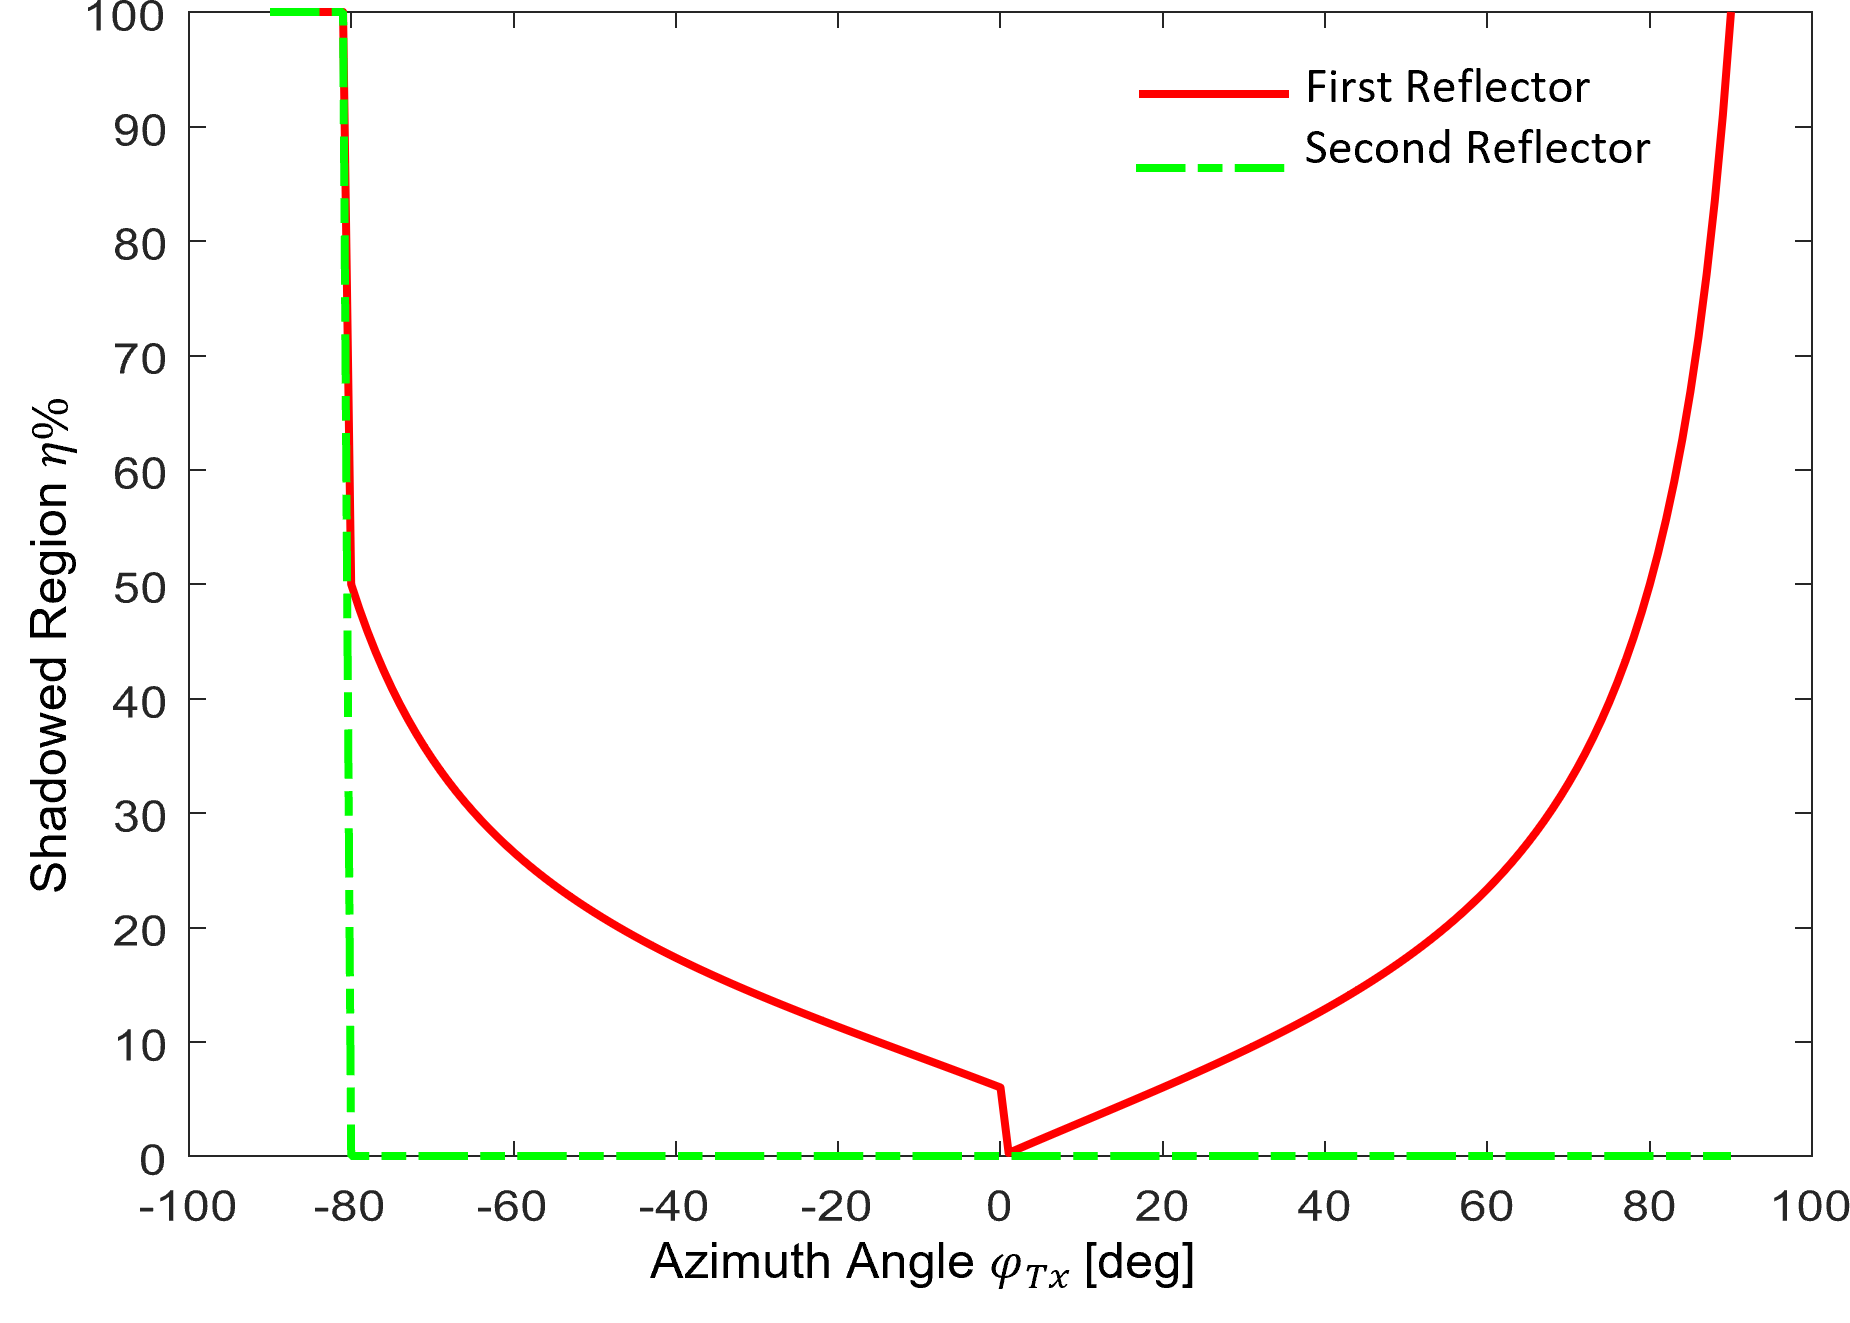
\includegraphics[width=0.7\linewidth]{images/Section 3 Images/ShadowRegion3}
	\caption{Plot depicting the amount of region shadowed for different incident azimuth angles $\varphi_{Tx} \in [-90:90]^\circ$ for simple case with  $\alpha_{m,n}=\alpha_{m,n+1}=\num{10}^\circ$ and $a_{m,n}=b_{m,n}=\SI{10}{\centi\meter}$ while $\beta_{m,n}=0^\circ$, and $\theta_{Tx}=0^\circ$. }
	\label{fig:Shadow region2}
\end{figure}
When one looks at the peak gain plot in \Cref{fig:arraymax_SR}, the transformational impact of this integration is evident when compared to the peak gain plot in \Cref{fig:arraymax}. After applying our modified model with the consideration of shadowed region $\eta_{a_{m,n}}$ and $\eta_{b_{m,n}}$, we achieved a significant improvement in the difference in peak gain between analytical and simulation models.

A noticeable difference of \SI{0.02}{\decibel} is observed between analytical model and EM simulation results at $\num{1}\times \num{8}$ HELIOS reflector array when compared to the results in \Cref{fig:arraymax} with \SI{0.4}{\decibel}. In similar manner, the difference of about \SI{0.2}{\decibel} at $\num{8}\times \num{8}$ HELIOS reflector array is observed instead of \SI{1.2}{\decibel} in \Cref{fig:arraymax}. This shows how accurate our analytical model is by now.
\begin{figure}[H]
	\centering
	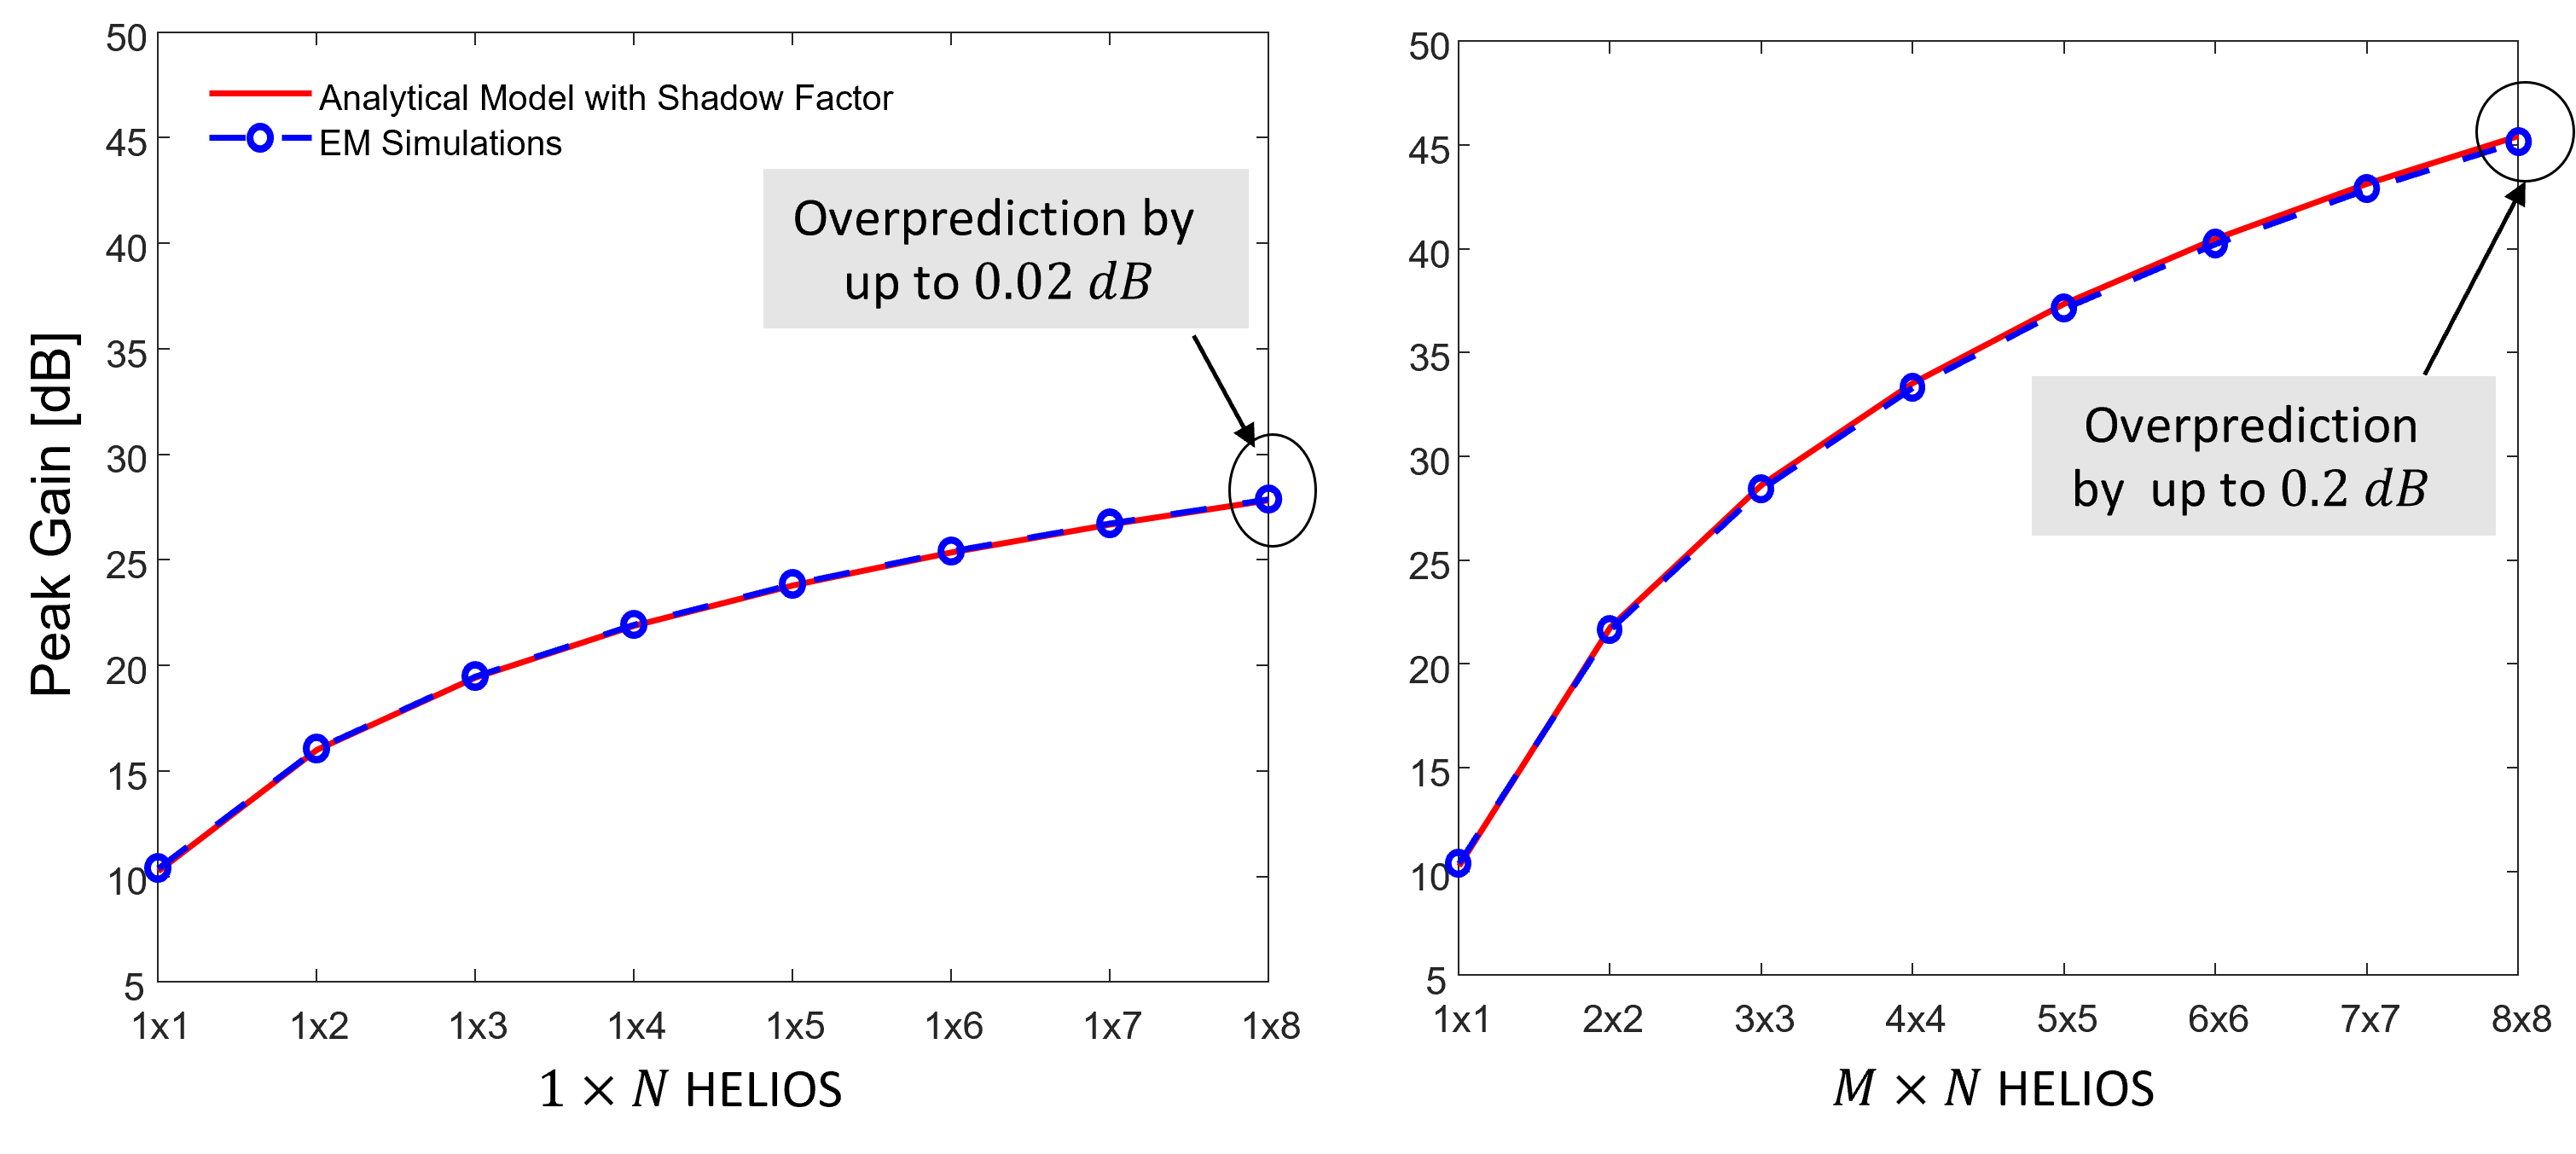
\includegraphics[width=1.0\linewidth]{images/Section 3 Images/Array_max_SR}
	\caption{Plot against HELIOS array and maximum gain between simulated and analytical model after the elimination of the shadowed region, highlighting the difference in maximum gain in $\si{\decibel}$ for the case when $a_{m,n}=b_{m,n}=\SI{10}{\centi\meter}$ and $\alpha_{m,n}=\beta_{m,n}=\num{10}^\circ$.}
	\label{fig:arraymax_SR}
\end{figure}
\section{Summary}
A brief overview of the prior section of \Cref{Simulation and Modeling of HELIOS Reflectors} is given in this section. The basic formulas that make up our analytical model are contained in \Cref{Eq:HELIOS_module} for an individual HELIOS module and by \Cref{Eq:HELIOS_array} for an array of HELIOS reflectors. \Cref{Improved Model using Inter-module Relations} improves our analytical model such that self-shadowing effects are accurately addressed. Important features are described, including the appearance of peak main lobe angles as determined by \Cref{HELIOS 2times beta}, and \Cref{HELIOS 2times alpha} and the beamwidth dependence of the module on dimensions $M$ and $N$ along the $y$ and $z$ axes, respectively. \Cref{Assessment of Differences between Simulations and Analytical Model} showcases the reflection behavior along different frequencies showing that the gain at higher frequencies is higher, but due to a more narrow reflection one needs to take more measures if one still wants to fairly distribute the reflection along a wider range of angles. Our comprehension is further enhanced by a brief comparison with the equations governing in \Cref{coordinate systems} showing the match between IRS and our analytical model.

The provided analytical model is actively used in \Cref{Performance Evaluation and Case Study} to forecast different communication channel features in various scenarios.
